\documentclass{article}
\usepackage{eason}
\usepackage{pdfpages}
\usepackage[a4paper, margin=1in]{geometry}

\newcommand{\scheduleSection}[3]{\noindent\textbf{#1}\\\noindent#3 \hfill[#2]\bigbreak}
\newcommand{\contentSection}[2]{\noindent#2 \hfill[#1]\bigbreak}

\numberwithin{equation}{section}

\newcommand{\Part}{IB}
\newcommand{\Department}{DPMMS}
\newcommand{\Course}{Optimisation}
\newcommand{\Term}{Easter Term}
\newcommand{\Year}{2026}
\newcommand{\Lecturer}{V. Jog}
\newcommand{\Repo}{ib-dpmms-optimisation-et-2026}

\newcommand{\DATE}{dummyDate}
\newcommand{\COMMITSHA}{dummySHA}
\title{Part \Part\space\Course \\ \vspace{0.5em}
\Large{Lectured by \Lecturer} \\ \vspace{0.5em}
\Large{Delivered by \Department}}
\author{Notes by Eason Shao}
\date{\Term\space\Year}

\begin{document}
\maketitle

\textbf{Disclaimer.} These notes are not official and are not endorsed by the lecturers. They are nowhere near accurate representations of what was lectured, and in particular, all errors are almost surely mine.

\textbf{Use of Artificial Intelligence.} I am grateful to AI tools, including GitHub Copilot (Student Edition), Claude by Anthropic, and ChatGPT, for their assistance with typesetting, diagrams, and checking for typos and inaccuracies. I take full responsibility for verifying the mathematical content of these notes.

\vspace{3em}

The source code is available at \GitHubHref{EasonSYC}{\Repo}.

This PDF is available at \href{https://tripos.easonshao.com}{https://tripos.easonshao.com}.

\tableofcontents

\section*{Schedules}
\label{sec:schedules}

\scheduleSection{Elements of convex optimisation}{3}{Convex sets and functions in \(\RR^n\), global and constrained optimality. Algorithms for unconstrained convex optimisation: gradient descent, Newton's algorithm. Introduction to convex optimisation on a convex set, the barrier method. Examples.}

\scheduleSection{Lagrangian methods \& duality}{3}{General formulation of constrained problems; the Lagrangian sufficiency theorem. Interpretation of La-grange multipliers as shadow prices. The dual linear problem, duality theorem in a standardized case, complementary slackness, dual variables and their interpretation as shadow prices. Relationship of the primal simplex algorithm to dual problem. Examples.}

\scheduleSection{Linear programming in the nondegenerate case}{3}{Convexity of feasible region; sufficiency of extreme points. Standardization of problems, slack variables, equivalence of extreme points and basic solutions. The primal simplex algorithm and the tableau. Examples.}

\scheduleSection{Applications of linear programming}{3}{Two person zero-sum games. Network flows; the max-flow min-cut theorem; the Ford--Fulkerson algorithm, the rational case. Network flows with costs, the transportation algorithm, relationship of dual variables with nodes. Examples. Conditions for optimality in more general networks. The formulation of simple practical and combinatorial problems as linear programming or network problems.}
\section*{Introduction}

Optimisation problems are of the following form.

\begin{problem}[Optimisation Problem]
    We want to minimise \(f\pqty{\vb{x}}\), subject to some constraints \(\vb{h}\pqty{\vb{x}} = \vb{b}\), for \(\vb{x} \in \mathcal{X}\).
\end{problem}

We may have some inequality constraint instead of an equality, with \(\vb{h}\pqty{\vb{x}} \leq \vb{b}\), and we impose this component-wise in higher dimensions.

In fact, inequalities constraints can be transformed into equality constraints, as
\[
    \vb{h}\pqty{\vb{x}} \leq \vb{b}
\]
is the same as
\[
    \vb{h}\pqty{\vb{x}} + \vb{s} = \vb{b}
\]
for \(\vb{s} \geq \vb{0}\), and we also minimise over \(\vb{s}\).

\begin{definition}[Terminology on Optimisation]
    \label{def:terminology}%
    The function \(\functiondomain{f}{\RR^n}{\RR}\) that we are trying to minimise is the \term{objective function}; \(\vb{h}\pqty{\vb{x}} = \vb{b}\) where \(\functiondomain{h}{\RR^n}{\RR^m}\) is a \term{functional constraint} with \(\vb{b} \in \RR^m\); and \(\mathcal{X}\) (often being \(\vb{x}\) being in the positive quadrant, or a cube/ball), is a \term{regional constraint}.

    The \(\vb{x}^*\) which solves the problem is called the \term{optimal solution}, and the value of the function at \(\vb{x}^*\), \(f\pqty{\vb{x}^*}\), is called the \term{optimal value/cost}.

    The set
    \[
        \mathcal{X}\pqty{\vb{b}} = \set{x \in \mathcal{X}}{\vb{h}\pqty{\vb{x}} = \vb{b}}
    \]
    is called the \term{feasible set}.

    The extra variables \(s\) are called \term{slack variables}.
\end{definition}

\section{Convex Optimisation}

\subsection{Convexity}

\subsubsection{Convex Functions}

\begin{definition*}[Convex Set]
    \label{def:convex-set}%
    A set \(S \subseteq \RR^n\) is \term{convex}, if for any \(\vb{x}, \vb{y} \in S\) and \(\lambda \in \ccintv{0}{1}\), we have
    \[
        \lambda \vb{x} + \pqty{1 - \lambda} \vb{y} \in S.
    \]
\end{definition*}

\autoref{def:convex-set} says that a set is convex, if and only if the straight line segment that connects any two points is contained in the set.

\begin{definition*}[Convex Function]
    \label{def:convex-fn}%
    A function \(\functiondomain{f}{S}{\RR}\) is a \term{convex} function, if \(S\) is convex, and for any \(\vb{x}, \vb{y} \in S\) and \(\lambda \in \ccintv{0}{1}\), we have
    \[
        f\pqty{\lambda \vb{x} + \pqty{1 - \lambda} \vb{y}} \leq \lambda f\pqty{\vb{x}} + \pqty{1 - \lambda} f\pqty{\vb{y}}.
    \]  
\end{definition*}

\begin{figure}[ht!]
    \centering
    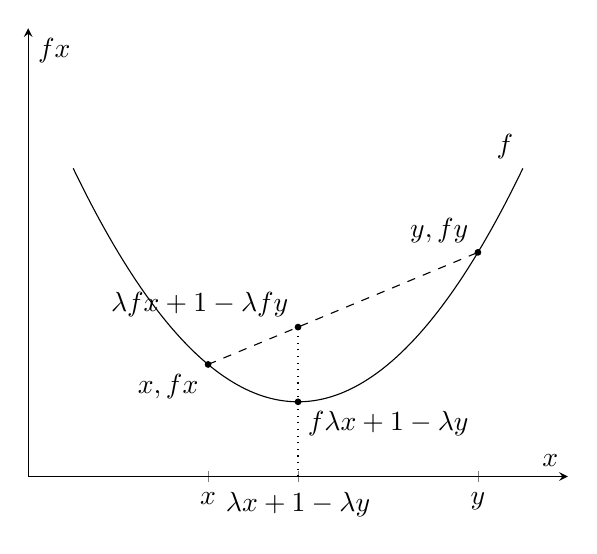
\begin{tikzpicture}
        \begin{axis}[
            axis lines = middle,
            xlabel = {\(x\)},
            ylabel = {\(f\pqty{x}\)},
            xmin = 0, xmax = 6,
            ymin = 0, ymax = 6,
            samples = 100,
            domain = 0.5:5.5,
            xtick = {2, 3, 5},
            xticklabels = {\(x\), \(\lambda x+\pqty{1-\lambda}y\), \(y\)},
            ytick = \empty
        ]

            \addplot[no marks] {0.5*(x-3)^2 + 1};
            \node[above left] at (axis cs:5.5,4.125) {\(f\)};

            \addplot[only marks, mark=*, mark size=1pt]
                coordinates {(2, 1.5) (5, 3)};

            \node[below left] at (axis cs:2, 1.5) {\(\pqty{x, f\pqty{x}}\)};
            \node[above left] at (axis cs:5, 3) {\(\pqty{y, f\pqty{y}}\)};

            \addplot[dashed] coordinates {(2, 1.5) (5, 3)};
            \addplot[only marks, mark=*, mark size=1pt]
                coordinates {(3, 2) (3, 1)};
            \node[above left] at (axis cs:3, 2) {\(\lambda f\pqty{x} + \pqty{1 - \lambda} f\pqty{y}\)};
            \node[below right] at (axis cs:3, 1) {\(f\pqty{\lambda x + \pqty{1 - \lambda} y}\)};

            \addplot[dotted] coordinates {(3, 0) (3, 2)};

        \end{axis}
    \end{tikzpicture}

    \caption{Convex Function}
    \label{fig:convex-fn}
\end{figure}

In other words, a convex function is a function whose chord lies above the curve.

\begin{remark}
    If \(-f\) is convex, then \(f\) is said to be concave. Linear functions are trivially both convex and concave.
\end{remark}

\subsubsection{First-Order Conditions}

\begin{figure}[ht!]
    \centering
    \begin{tikzpicture}
        \begin{axis}[
            axis lines = middle,
            xlabel = {\(x\)},
            ylabel = {\(f(x)\)},
            xmin = -1, xmax = 5,
            ymin = -2, ymax = 9,
            xtick = \empty,
            ytick = \empty,
            domain = 0:4,
            samples = 100,
            width = 10cm
        ]

            \addplot[no marks, thick, blue] {0.5*x^2};

            \addplot[only marks, mark=*, mark size = 1pt] coordinates {(1, 0.5) (2, 2) (3, 4.5)};

            \addplot[domain=0.25:4.5] {1 * (x - 1) + 0.5};
            \addplot[domain=0.4:4.2] {2 * (x - 2) + 2};
            \addplot[domain=0.5:4.1] {3 * (x - 3) + 4.5};
        \end{axis}
    \end{tikzpicture}

    \caption{Convex Function and its Tangents}
    \label{fig:convex-fn-tangents}
\end{figure}

We study in this section functions that are differentiable. By observing \autoref{fig:convex-fn-tangents}, it seems like the graph of a function always lie above its tangents, so we have
\[
    f\pqty{y} \geq f\pqty{x} + \pqty{y - x} f'\pqty{x}.
\]

In higher dimensions, we should have
\[
    f\pqty{\vb{y}} \geq f\pqty{\vb{x}} + \pqty{\vb{y} - \vb{x}} \transpose \grad f\pqty{\vb{x}}.
\]

\begin{theorem}[First-Order Condition]
    \label{thm:first-order-condition}%
    A differentiable function \(\functiondomain{f}{\RR^n}{\RR}\) is convex, if and only if for all \(\vb{x}, \vb{y} \in \RR^n\), we have
    \[
        f\pqty{\vb{y}} \geq f\pqty{\vb{x}} + \pqty{\vb{y} - 
        \vb{x}}\transpose \grad f\pqty{\vb{x}}.
    \]  
\end{theorem}

\begin{remark}
    If at \(x\), \(\grad f\pqty{x} = \vb{0}\), then \(x\) is a minimiser of \(f\).
\end{remark}

\begin{proof}
    We first suppose the function is convex. When \(n = 1\), we have
    \[
        f\pqty{x + t \pqty{y - x}} \leq \pqty{1 - t} f\pqty{x} + t f\pqty{y}
    \]
    for all \(t \in \ccintv{0}{1}\). This means
    \[
        f\pqty{y} \geq f\pqty{x} + \frac{f\pqty{x + t \pqty{y - x}} - f\pqty{x}}{t}.
    \]

    Taking the limit as \(t \to 0\),
    \[
        f\pqty{y} \geq f\pqty{x} + \pqty{y - x} f'\pqty{x}.
    \]

    To resolve the general case, for \(\vb{x}, \vb{y} \in \RR^n\), set
    \[
        g\pqty{t} = f\pqty{\pqty{1 - t} \vb{x} + t \vb{y}},
    \]  
    and \(g\) is a convex function with \(\functiondomain{g}{\ccintv{0}{1}}{\RR}\). Using the one-dimensional result, we have
    \[
        g\pqty{1} \geq g\pqty{0} + \pqty{1 - 0} g'\pqty{0}.
    \]

    Therefore.
    \[
        f\pqty{\vb{y}} \geq f\pqty{\vb{x}} + \grad f\pqty{\vb{x}} \transpose \pqty{\vb{y} - \vb{x}}.
    \]

    Now we prove the converse. Set
    \[
        \vb{x}_t = \pqty{1 - t} \vb{x} + t\vb{y}.
    \]

    First-order conditions imply that
    \begin{align*}
        f\pqty{\vb{x}} &\geq f\pqty{\vb{x}_t} + \grad f\pqty{\vb{x}_t} \transpose \pqty{\vb{x} - \vb{x}_t}, \\
        f\pqty{\vb{y}} &\geq f\pqty{\vb{x}_t} + \grad f\pqty{\vb{x}_t} \transpose \pqty{\vb{y} - \vb{x}_t}.
    \end{align*}

    Multiplying the first inequality by \(\pqty{1 - t}\) and the second by \(t\), and adding together, we have
    \[
        \pqty{1 - t} f\pqty{\vb{x}} + t f\pqty{\vb{y}} \geq f\pqty{\vb{x}_t} + 0 = f\pqty{\pqty{1 - t} \vb{x} + t \vb{y}}.
    \]
\end{proof}

\subsubsection{Second-Order Conditions}

We return to \autoref{fig:convex-fn-tangents}. We note that it seems that the slope of the gradient is increasing, so it means that \(f'' \geq 0\). But we shall generalise this to higher dimensions. For this, we recall the \term{Hessian matrix}
\[
    \bqty{\grad^2 f\pqty{\vb{x}}}_{ij} = \pdv{f\pqty{\vb{x}}}{x_i}{x_j}.
\]

Recall that the one-dimensional Taylor series takes the form
\[
    f\pqty{y} = f\pqty{x} + \pqty{y - x} f'\pqty{x} + \frac{\pqty{y - x}^2}{2} f''\pqty{x} + \cdots
\]
and similarly, in the \(n\)-dimensional case, the Taylor series will have the form
\[
    f\pqty{\vb{y}} = f\pqty{\vb{x}} + \pqty{\vb{y} - \vb{x}}\transpose \grad f\pqty{\vb{x}} + \frac{1}{2} \pqty{\vb{y} - \vb{x}}\transpose \grad^2 f\pqty{\vb{x}} \pqty{\vb{y} - \vb{x}} + \cdots
\]

The proof is simple. If we apply the one-dimensional Taylor series to the function
\[
    g\pqty{t} = f\pqty{\vb{x} + \pqty{\vb{y} - \vb{x}} t},
\]
then
\[
    g\pqty{1} = g\pqty{0} + g'\pqty{0} + \frac{1}{2} g''\pqty{0} + \cdots
\]
so
\[
    f\pqty{\vb{y}} = f\pqty{\vb{x}} + \grad f\pqty{x} \transpose \pqty{\vb{y} - \vb{x}} + \frac{1}{2} \pqty{\vb{y} - \vb{x}} \transpose \grad^2 f\pqty{x} \pqty{\vb{y} - \vb{x}}.
\]

\begin{theorem}[Second-Order Condition]
    \label{thm:second-order-condition}%
    A twice-differentiable function \(\functiondomain{f}{\RR^n}{\RR}\) is convex, if and only if
    \[
        \grad^2 f\pqty{x} \posDefEq 0
    \]
    for all \(x \in \RR^n\).
\end{theorem}

\begin{remark}
    We say a symmetric \(n\)-dimensional matrix \(A\) is \term{positive semi-definite}, denoted \(A \posDefEq 0\), if
    \[
        \vb{x}\transpose A \vb{x} \geq 0
    \]
    for all \(\vb{x} \in \RR^n\). Equivalently, all \(n\) eigenvalues of \(A\) are non-negative.
\end{remark}

\begin{proof}[\proofname\ (One Direction Only)]
    We prove convexity from positive semi-definiteness. For any \(\vb{x}\) and \(\vb{y}\), we have for some \(\vb{z} \in \RR^n\) (by the intermediate value theorem),
    \begin{align*}
        f\pqty{\vb{y}} &= f\pqty{\vb{x}} + \grad f\pqty{\vb{x}} \transpose \pqty{\vb{y} - \vb{x}} + \frac{1}{2} \pqty{\vb{y} - \vb{x}} \transpose \grad^2 f\pqty{\vb{z}} \pqty{\vb{y} - \vb{x}} \\
        &\geq f\pqty{\vb{x}} + \grad f\pqty{\vb{x}} \transpose \pqty{\vb{y} - \vb{x}}
    \end{align*}

    This implies the first-order condition, so by \autoref{thm:first-order-condition}, \(f\) is convex.
\end{proof}

\subsection{Gradient Descent Algorithm}

We observe that
\[
    f\pqty{\vb{y}} \approx f\pqty{\vb{x}} + \grad f\pqty{\vb{x}} \transpose \pqty{\vb{y} - \vb{x}}.
\]

Say we have
\[
    \vb{y} - \vb{x} = - \epsilon \grad f\pqty{\vb{x}}
\]
where \(0 < \epsilon \ll 1\) is small. Then we have
\begin{align*}
    f\pqty{\vb{y}} &\approx f\pqty{\vb{x}} + \grad f\pqty{\vb{x}} \transpose \pqty{- \epsilon \grad f \pqty{\vb{x}}} \\
    &= f\pqty{\vb{x}} - \epsilon \norm{\grad f\pqty{\vb{x}}}^2.
\end{align*}

This leads to the gradient descent algorithm, as described in \autoref{alg:gradient-descent}.

\begin{algorithm}[ht!]
    \caption{Gradient Descent Algorithm}\label{alg:gradient-descent}%
    \begin{algorithmic}
        \Function{GradientDescent}{\(f, \vb{x}_0\)}
        \State \(t \gets 0\)
        \Repeat
            \State \(\vb{v}_t \gets - \grad f\pqty{\vb{x}_t}\)
            \State Choose Step Size \(\eta_t > 0\)
            \State \(\vb{x}_{t + 1} \gets \vb{x}_t + \eta_t \vb{v}_t\)
            \State \(t \gets t + 1\)
        \Until{Certain Stopping Criteria(s)}
        \State \Return{\(\vb{x}_{t}\)}
        \EndFunction
    \end{algorithmic}
\end{algorithm}

\begin{remark}
    The stopping criteria can be, for example, when our computing power runs out, or when the gradient is very small.
\end{remark}

We note that the gradient descent algorithm could fail: if the step size is too large, we might not necessarily reach the minimum, for example, we overshoot if the function is very steep. Similar issues appear when the step size is too small, for example, it will take very long to reach the minimum if the function is very flat. 

\begin{figure}[ht!]
    \centering
    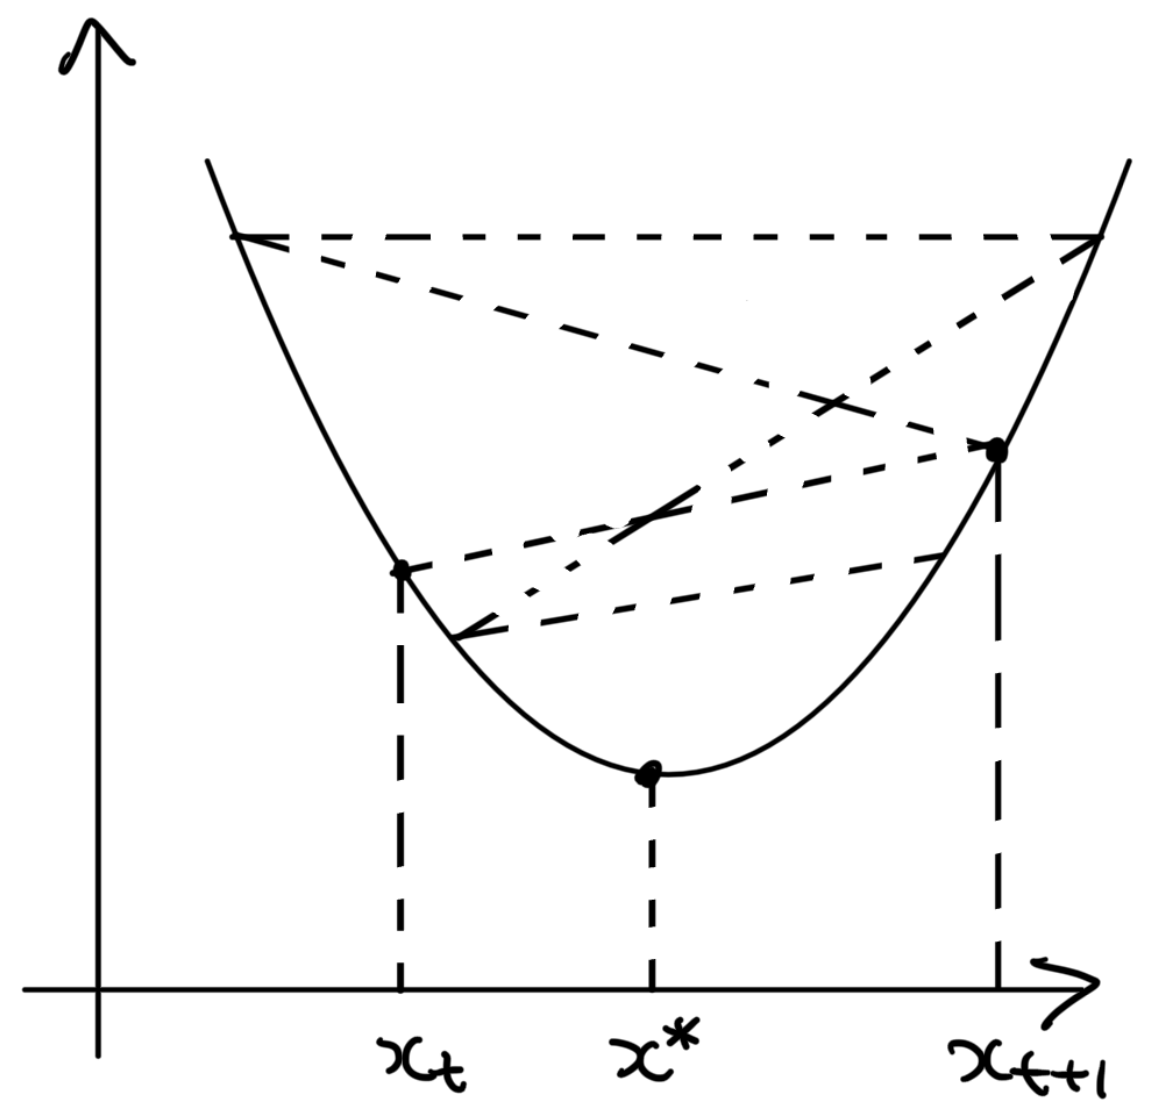
\includegraphics[width=0.5\linewidth]{fig/gradient-descent-overshoot.png}
    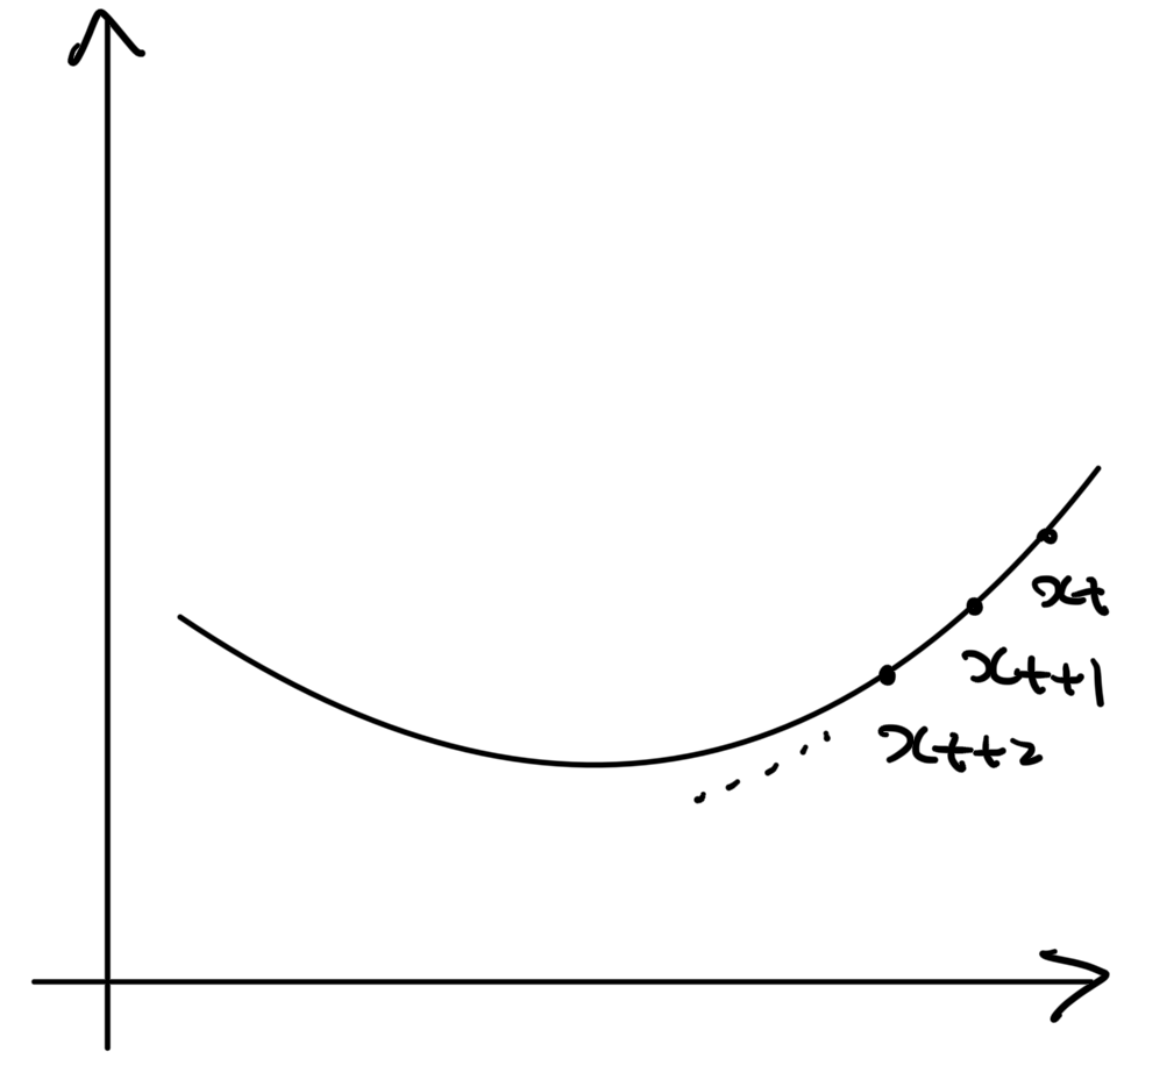
\includegraphics[width=0.5\linewidth]{fig/gradient-descent-undershoot.png}
    \caption{Step Sizes in Gradient Descent}
    \label{fig:gradient-descent-step-sizes}%
\end{figure}

Therefore, we restrict our class of functions.

\subsubsection{Smoothness and Strong Convexity}

\begin{definition}[\(\alpha\)-strong convexity, \(\beta\)-smooth]
    \label{def:alpha-sc-beta-smooth}%
    Let \(\alpha, \beta > 0\). A twice-differentiable function \(\functiondomain{f}{\RR^n}{\RR}\) is \term{\(\beta\)-smooth} if \(\grad^2 f\pqty{\vb{x}} \negDefEq \beta I\) for all \(\vb{x} \in \RR^n\); and is \term{\(\alpha\)-strongly convex} if \(\grad^2 f\pqty{\vb{x}} \posDefEq \alpha I\) for all \(\vb{x} \in \RR^n\).
\end{definition}

\begin{remark}
    We say two matrices \(A \negDefEq B\), if \(B - A \posDefEq 0\), i.e., \(B - A\) is a positive semi-definite matrix. This implies \(\vb{x}\transpose A \vb{x} \leq \vb{x} \transpose B \vb{x}\) for all \(\vb{x} \in \RR^n\).
\end{remark}

In other words, this condition states that the eigenvalues are at most \(\beta\), or at least \(\alpha\). Upper bounding by \(\beta\) rules out very steep functions, and lower bounding by \(\alpha\) rules out very flat functions.

\begin{theorem}[Second-Order (Quadratic) Bounds]
    \label{thm:second-order-quadratic-bounds}%
    Let \(\functiondomain{f}{\RR^n}{\RR}\) be twice-differentiable and \(\vb{x}, \vb{y} \in \RR^n\).

    \begin{itemize}
        \item If \(f\) is \(\beta\)-smooth, then
        \[
            f\pqty{\vb{y}} \leq f\pqty{\vb{x}} + \grad f\pqty{\vb{x}}\transpose \pqty{\vb{y} - \vb{x}} + \frac{\beta}{2} \norm{\vb{y} - \vb{x}}^2.
        \]

        \item If \(f\) is \(\alpha\)-strongly convex, then
        \[
            f\pqty{\vb{y}} \geq f\pqty{\vb{x}} + \grad f\pqty{\vb{x}}\transpose \pqty{\vb{y} - \vb{x}} + \frac{\alpha}{2} \norm{\vb{y} - \vb{x}}^2.
        \]
    \end{itemize}
\end{theorem}

We are essentially bounding the function \(f\) between two quadratics -- the \(\beta\) as an upper bound, and the \(\alpha\) as a lower bound, as in \autoref{fig:quadratic-bounds} -- and quadratic functions are easier to understand!

\begin{figure}[ht!]
    \centering
    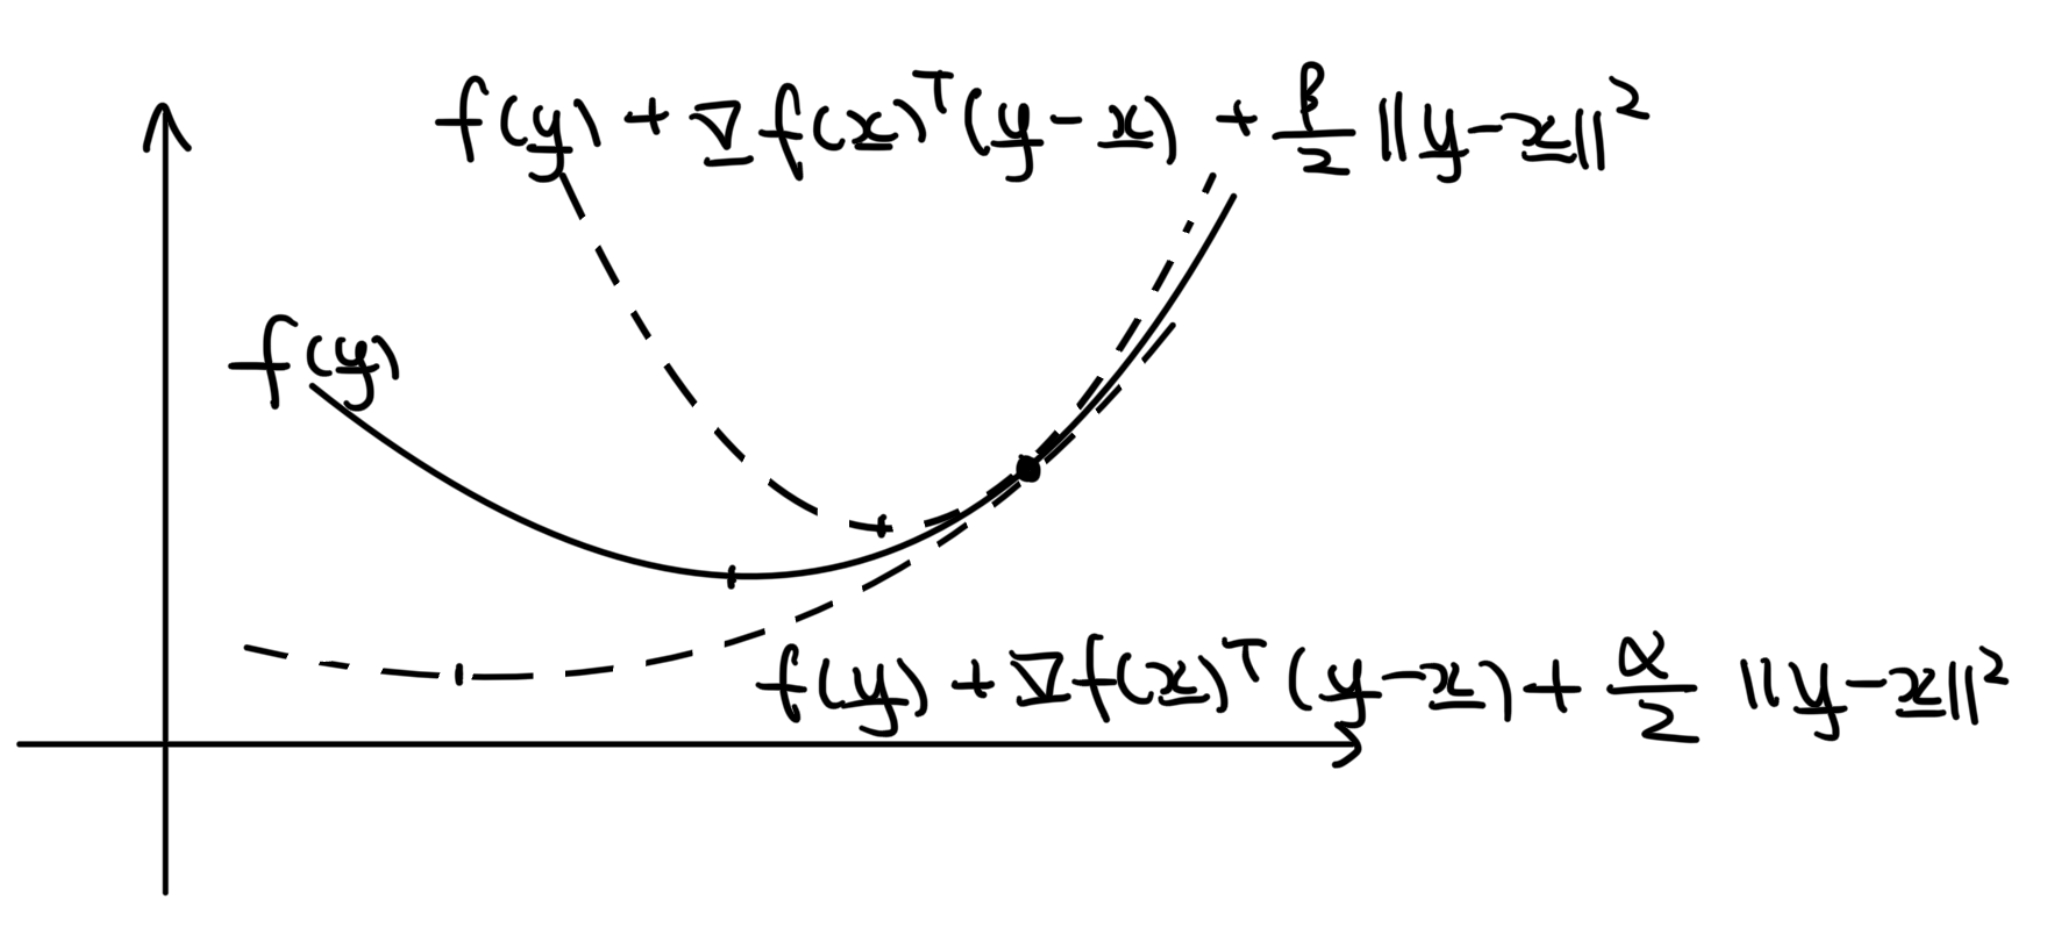
\includegraphics[width=0.8\linewidth]{fig/quadratic-approximation.png}
    \caption{Quadratic Bounds}
    \label{fig:quadratic-bounds}%
\end{figure}

\begin{proof}
    We use the multivariate Taylor series expansion. Expanding around \(\vb{x}\), we have
    \[
        f\pqty{\vb{y}} = f\pqty{\vb{x}} + \grad f\pqty{\vb{x}} \transpose \pqty{\vb{y} - \vb{x}} + \frac{1}{2} \pqty{\vb{y} - \vb{x}}\transpose \grad^2 f\pqty{\vb{z}} \pqty{\vb{y} - \vb{x}}
    \]
    where \(\vb{z}\) is some point on the line segment joining \(\vb{x}\) and \(\vb{y}\).

    Now, observe that if \(f\) is \(\beta\)-smooth,
    \[
        \frac{1}{2} \pqty{\vb{y} - \vb{x}}\transpose \grad^2 f\pqty{\vb{z}} \pqty{\vb{y} - \vb{x}} \leq \frac{1}{2} \pqty{\vb{y} - \vb{x}}\transpose \pqty{\beta I} \pqty{\vb{y} - \vb{x}} = \frac{\beta}{2} \norm{\vb{y} - \vb{x}}^2,
    \]
    and similarly, if \(f\) is \(\alpha\)-strongly convex,
    \[
        \frac{1}{2} \pqty{\vb{y} - \vb{x}}\transpose \grad^2 f\pqty{\vb{z}} \pqty{\vb{y} - \vb{x}} \geq \frac{1}{2} \pqty{\vb{y} - \vb{x}}\transpose \pqty{\alpha I} \pqty{\vb{y} - \vb{x}} = \frac{\alpha}{2} \norm{\vb{y} - \vb{x}}^2.
    \]
\end{proof}

Two very important corollaries are as follows.

\begin{corollary}[Sufficiently Small Step Size]
    \label{cor:grad-descent-beta-bound}%
    If \(f\) is \(\beta\)-smooth, then
    \[
        f\pqty{\vb{x} - \frac{1}{\beta} \grad f\pqty{\vb{x}}} \leq f\pqty{\vb{x}} - \frac{1}{2 \beta} \norm{\grad f\pqty{\vb{x}}}^2.
    \]
\end{corollary}

This basically states that if our function is sufficiently flat (\(\beta\)-smooth) (i.e. its sharpness is controlled), then a step size of \(\flatfrac{1}{\beta}\) is small enough to ensure we are always descending (and not overshoot)

\begin{proof}
    Substitute \(\vb{y} = \vb{x} - \flatfrac{\grad f\pqty{\vb{x}}}{\beta}\) into \autoref{thm:second-order-quadratic-bounds}.
\end{proof}

\begin{corollary}[Upper Bound on Difference to Minimum]
    \label{cor:grad-descent-alpha-bound}%
    Let \(f\) is \(\alpha\)-strongly convex, and let \(f\pqty{\vb{x}^{\ast}}\) be the minimum of \(f\). Then for any \(\vb{x}\), we have
    \[
        f\pqty{\vb{x}^{\ast}} \geq f\pqty{\vb{x}} - \frac{1}{2 \alpha} \norm{\grad f\pqty{\vb{x}}}^2.
    \]

    Equivalently,
    \[
        f\pqty{\vb{x}} - f\pqty{\vb{x}^{\ast}} \leq \frac{1}{2 \alpha} \norm{\grad f\pqty{\vb{x}}}^2.
    \]
\end{corollary}

This basically states that if our function is sufficiently steep (\(\alpha\)-strongly convex) (i.e. its flatness is controlled), then we have a bound on the distance (measured in the function value) to the minimum. If \(\norm{\grad f\pqty{\vb{x}}}^2 \leq 2 \alpha \epsilon\), then \(\vb{x}\) is optimal up to \(\epsilon\) error. This allows us to control the error, even for very flat functions.

\begin{proof}
    By \autoref{thm:second-order-quadratic-bounds}, we have
    \[
        f\pqty{\vb{y}} \geq f\pqty{\vb{x}} + \grad f\pqty{\vb{x}}\transpose \pqty{\vb{y} - \vb{x}} + \frac{\alpha}{2} \norm{\vb{y} - \vb{x}}^2.
    \]

    We take the minimum over \(\vb{y}\) on both sides. Then
    \[
        f\pqty{\vb{x}^{\ast}} \geq \min_{\vb{y} \in \RR^n} \bqty{f\pqty{\vb{x}} + \grad f\pqty{\vb{x}}\transpose \pqty{\vb{y} - \vb{x}} + \frac{\alpha}{2} \norm{\vb{y} - \vb{x}}^2}.
    \]

    Differentiating with respect to \(\vb{y}\) on the right-hand side gives
    \[
        \grad f\pqty{\vb{x}} + \alpha \pqty{\vb{y} - \vb{x}}
    \]
    as the gradient, and setting this equal to zero gives
    \[
        \vb{y} = \vb{x} - \frac{1}{\alpha} \grad f\pqty{\vb{x}}.
    \]

    Call this \(\vb{y}^{\ast}\). Plug this back into \autoref{thm:second-order-quadratic-bounds}, we have
    \[
        f\pqty{\vb{x}^{\ast}} \geq f\pqty{\vb{x}} - \frac{1}{2\alpha} \norm{\grad f\pqty{\vb{x}}}^2
    \]
    as desired.
\end{proof}

\subsubsection{Convergence of Gradient Descent}

\begin{theorem}[Exponentially-Fast Bound of Distance to Minimum]
    \label{thm:exp-bound-dist-minimum}%
    Let \(f\) be \(\alpha\)-strongly convex and \(\beta\)-smooth. Suppose \(f\) is minimised at \(\vb{x}^{\ast}\). Then gradient descent with a fixed step size of \(\eta_t = \frac{1}{\beta}\) satisfies
    \[
        f\pqty{\vb{x}_T} - f\pqty{\vb{x}^{\ast}} \leq \pqty{1 - \frac{\alpha}{\beta}}^{T} \pqty{f\pqty{\vb{x}_0} - f\pqty{\vb{x}^{\ast}}} \leq e^{- \flatfrac{\alpha T}{\beta}} \pqty{f\pqty{\vb{x}_0} - f\pqty{\vb{x}^{\ast}}}.
    \]
\end{theorem}

\begin{remark}
    The second inequality simply comes from \(e^{-x} \geq 1 - x\).
\end{remark}

In other words, taking
\[
    T \geq \frac{\beta}{\alpha} \log \pqty{\frac{f\pqty{\vb{x}_0} - f\pqty{\vb{x}^{\ast}}}{\epsilon}}
\]
gives an \(\epsilon\)-optimal point. This type of convergence is called \term{linear convergence} in optimisation literature -- this is a good benchmark, since \(\log\) is `like a constant' in computer science, so if you have an algorithm that converges like \(\log\), then it is really good.

\begin{proof}
    Observe that
    \begin{align*}
        f\pqty{\vb{x}_{t + 1}} - f\pqty{\vb{x}^{\ast}} &\leq f\pqty{\vb{x}_t} - f\pqty{\vb{x}^{\ast}} - \frac{1}{2\beta} \norm{\grad f\pqty{\vb{x}_t}}^2 && \text{\autoref{cor:grad-descent-beta-bound}} \\
        &\leq f\pqty{\vb{x}_t} - f\pqty{\vb{x}^{\ast}} - \frac{\alpha}{\beta} \pqty{f\pqty{\vb{x}_t} - f\pqty{\vb{x}^{\ast}}} && \text{\autoref{cor:grad-descent-alpha-bound}} \\
        &= \pqty{1 - \frac{\alpha}{\beta}} \pqty{f\pqty{\vb{x}_t} - f\pqty{\vb{x}^{\ast}}}.
    \end{align*}

    This reduces to our desired result by telescoping.
\end{proof}

\begin{example}[Gradient Descent might Converge Unnecessarily Slowly]
    Suppose in \(\RR^2\), let
    \[
        f\pqty{\vb{x}} = \frac{1}{2} \pqty{x_1^2 + 100 x_2^2}.
    \]

    Then
    \[
        \grad^2 f\pqty{\vb{x}} = \bmqty{\dmat{1,100}}.
    \]

    Then \(\alpha = 1\) and \(\beta = 100\), but
    \[
        1 - \frac{\alpha}{\beta} = 0.99
    \]
    is very close to \(1\). This number \(\flatfrac{\alpha}{\beta}\) is too small -- and this means this converges very slowly, when all we have to do is to rescale the variables!
\end{example}

In optimisation theory, we usually first scale/change basis of the function, in order to make sure no axis are especially badly behaved. This is called \term{pre-conditioning}.

\begin{remark}
    The recursion step
    \[
        \vb{x}_{t + 1} = \vb{x}_t - \frac{1}{\beta} \grad f\pqty{\vb{x}_t}
    \]
    precisely minimises the upper bound quadratic.
\end{remark}

\subsection{Newton's Method}

We take a second-order Taylor approximation at \(\vb{x}\), which reads
\[
    f\pqty{\vb{y}} = f\pqty{\vb{x}} + \grad f\pqty{\vb{x}}\transpose \pqty{\vb{y} - \vb{x}} + \frac{1}{2} \pqty{\vb{y} - \vb{x}}\transpose \grad^2 f\pqty{\vb{x}} \pqty{\vb{y} - \vb{x}}.
\]

We change the update rule to
\[
    \vb{x}_{t + 1} = \argmin_{\vb{y} \in \RR^n} \bqty{f\pqty{\vb{x}_t} + \grad f\pqty{\vb{x}_t}\transpose \pqty{\vb{y} - \vb{x}_t} + \frac{1}{2} \pqty{\vb{y} - \vb{x}_t}\transpose \grad^2 f\pqty{\vb{x}_t} \pqty{\vb{y} - \vb{x}_t}}.
\]

Taking the gradient gives
\[
    \vb{0} = \grad f\pqty{\vb{x}_t} + \grad^2 f\pqty{\vb{x}_t} \pqty{\vb{y} - \vb{x}_t}.
\]

This solves to
\[
    \vb{y} = \vb{x}_t - \pqty{\grad^2 f\pqty{\vb{x}_t}}\inverse \grad f\pqty{\vb{x}_t}.
\]

\subsubsection{Newton's Algorithm}

This is called \term{Newton's Algorithm}, and is outlined in \autoref{alg:newtons-algorithm}.

\begin{algorithm}[ht!]
    \caption{Newton's Algorithm}\label{alg:newtons-algorithm}%
    \begin{algorithmic}
        \Function{NewtonAlgorithm}{\(f, \vb{x}_0\)}
        \State \(t \gets 0\)
        \Repeat
            \State \(\vb{x}_{t + 1} \gets \vb{x}_t - \pqty{\grad^2 f\pqty{\vb{x}_t}}\inverse \grad f\pqty{\vb{x}_t}\)
            \State \(t \gets t + 1\)
        \Until{Certain Stopping Criteria(s)}
        \State \Return{\(\vb{x}_{t}\)}
        \EndFunction
    \end{algorithmic}
\end{algorithm}

The one-dimensional case is familiar in A-Level context -- the Newton--Raphson method is a root finding algorithm for \(f'\pqty{x} = g\pqty{x}\):
\[
    x_{t + 1} = x_t - \frac{g\pqty{x_t}}{g'\pqty{x_t}}.
\]

\begin{figure}[ht!]
    \centering
    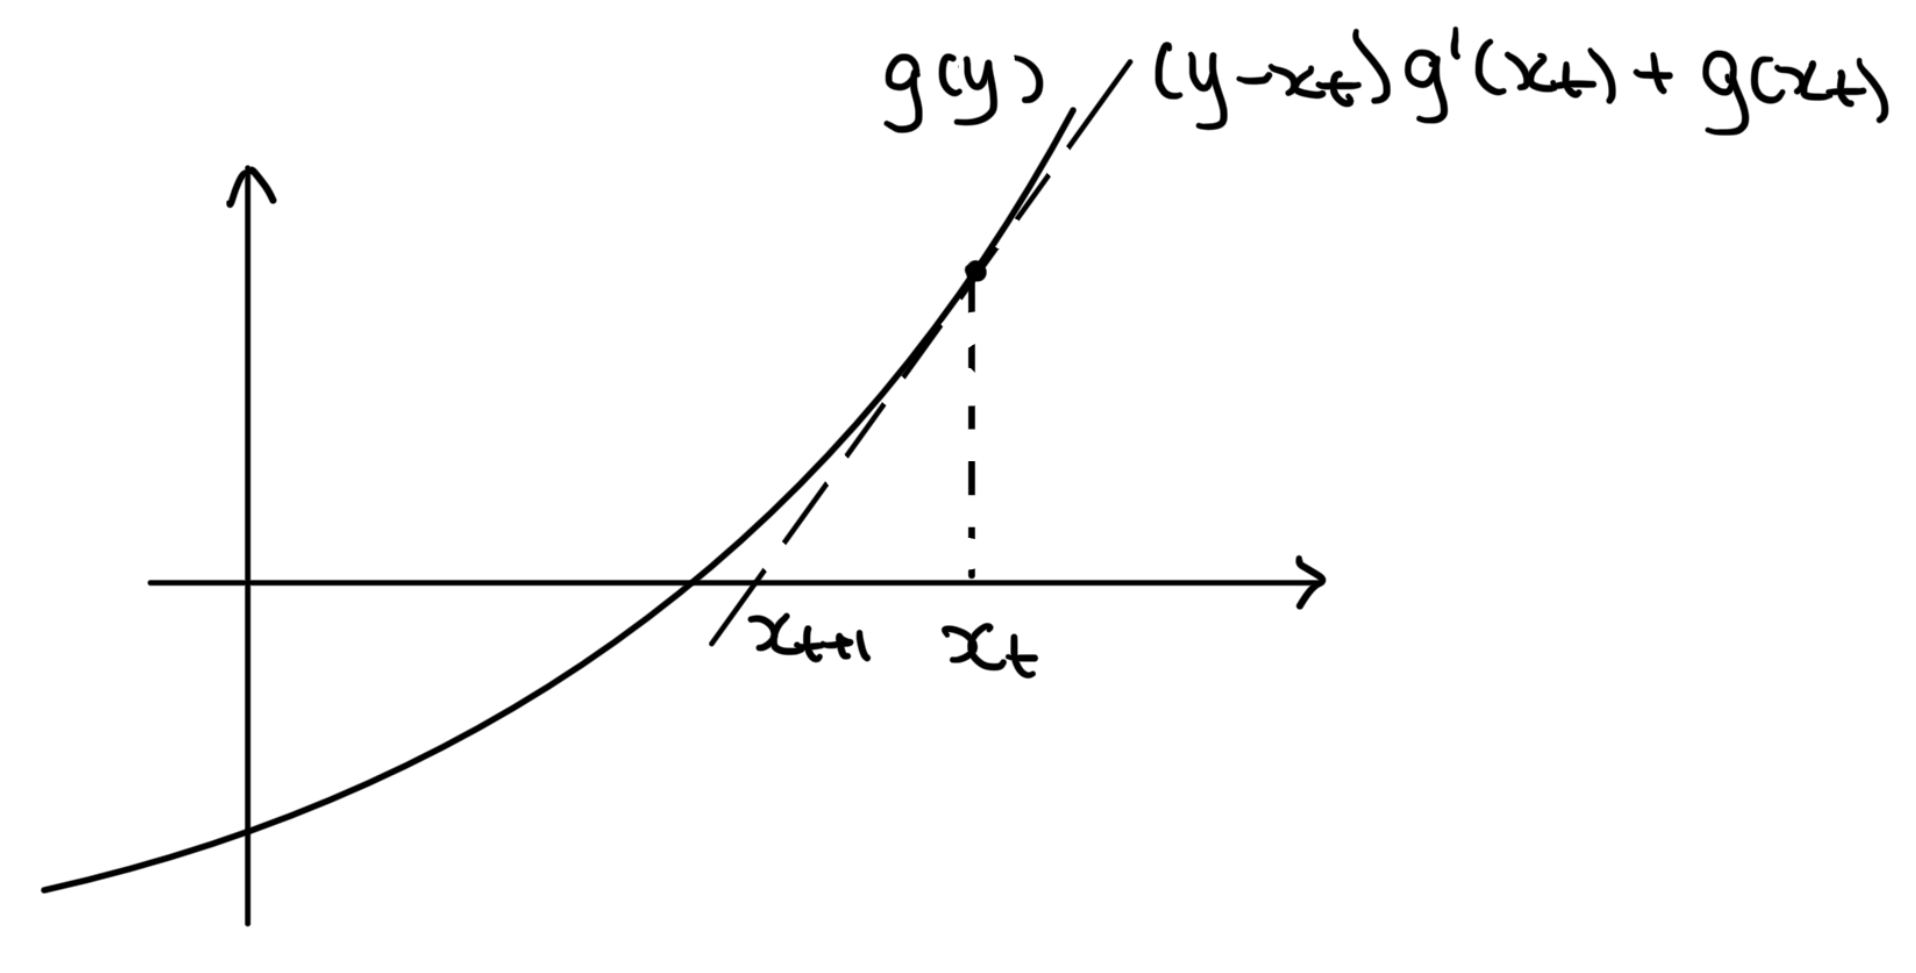
\includegraphics[width=0.8\linewidth]{fig/newton-raphson.png}
    \caption{Newton--Raphson Method}
    \label{fig:newton-raphson}%
\end{figure}

\begin{definition}[Matrix Norm]
    \label{def:matirx-norm}%
    For a matrix \(A \in \RR^{n \times n}\), \(\norm{A}\) is the smallest \(a > 0\), such that
    \[
        \norm[2]{A\vb{z}} \leq a \norm[2]{\vb{z}}
    \]
    for all \(\vb{z} \in \RR^n\), where \(\norm[2]{\cdot}\) denotes the usual \(\ell^2\)-norm on \(\RR^n\). For positive semi-definite matrices \(A\), this is simply the largest eigenvalue.
\end{definition}

\begin{theorem}[Convergence Condition for Newton's Method]
    \label{thm:newton-algorithm-convergence}%
    Suppose \(f\) is a twice-differentiable \(\alpha\)-strongly convex function that has an \(\ell\)-Lipschitz Hessian, i.e., for all \(\vb{x}, \vb{y} \in \RR^n\), we have
    \[
        \norm{\grad^2 f\pqty{\vb{x}} - \grad^2 f\pqty{\vb{y}}} \leq \ell \norm[2]{\vb{x} - \vb{y}}.
    \]

    Then Newton's Method satisfies
    \[
        f\pqty{\vb{x}_k} - f\pqty{\vb{x}^{\ast}} \leq \pqty{\frac{2 \alpha^3}{\ell^2}} \pqty{\frac{\ell}{2 \alpha^2} \norm[2]{\grad f\pqty{\vb{x}_0}}}^{2^{k + 1}}.
    \]
\end{theorem}

\begin{remark}
    Suppose
    \[
        \norm[2]{\grad f\pqty{\vb{x}_0}} < \frac{2 \alpha^2}{\ell},
    \]
    then the number of steps required goes down to \(\log \log\) -- compared to \(\log\) in gradient descent, which is exponentially faster. But we need to be at a good enough point at the beginning, otherwise this does not necessarily converge.
\end{remark}

\begin{example}[Application in Machine Learning]
    Suppose we have data points \(\pqty{x_1, y_1}, \pqty{x_2, y_2}, \ldots, \pqty{x_n, y_n}\). Most machine learning algorithms are trying to minimise
    \[
        \min_{\theta} \sum_{i = 1}^{n} \ell\pqty{f_{\theta} \pqty{x_i}, y_i}
    \]
    where \(\ell\) is a suitable loss function. But we almost always use gradient descent, rather than Newton's method.
\end{example}

A huge drawback of Newton's algorithm is we need to calculate the Hessian of a function -- which is a \(n \times n\) matrix. This takes up much larger computational power compared to simply calculating the gradient. Although it is a good method, we cannot run it at a large scale.

In theory, one could possibly use the best cubic, quartic, \dots approximations at a point, and go on and on, but the third order term
\[
    \frac{\partial^3 f}{\partial x_i \partial x_j \partial x_k} \pqty{y_i - x_i} \pqty{y_j - x_j} \pqty{y_k - x_k}
\]
is a nightmare to optimise.

\subsubsection{Barrier Method}

Suppose we want to optimise \(f\pqty{\vb{x}}\) subject to some constraints
\[
    \vb{a}_i \transpose \vb{x} \leq \vb{b}_i
\]
for \(1 \leq i \leq m\), where \(f\) is convex. This is a \textbf{constrained} optimisation problem -- so trivially applying gradient descent or Newton's method will not work.

\begin{figure}[ht!]
    \centering
    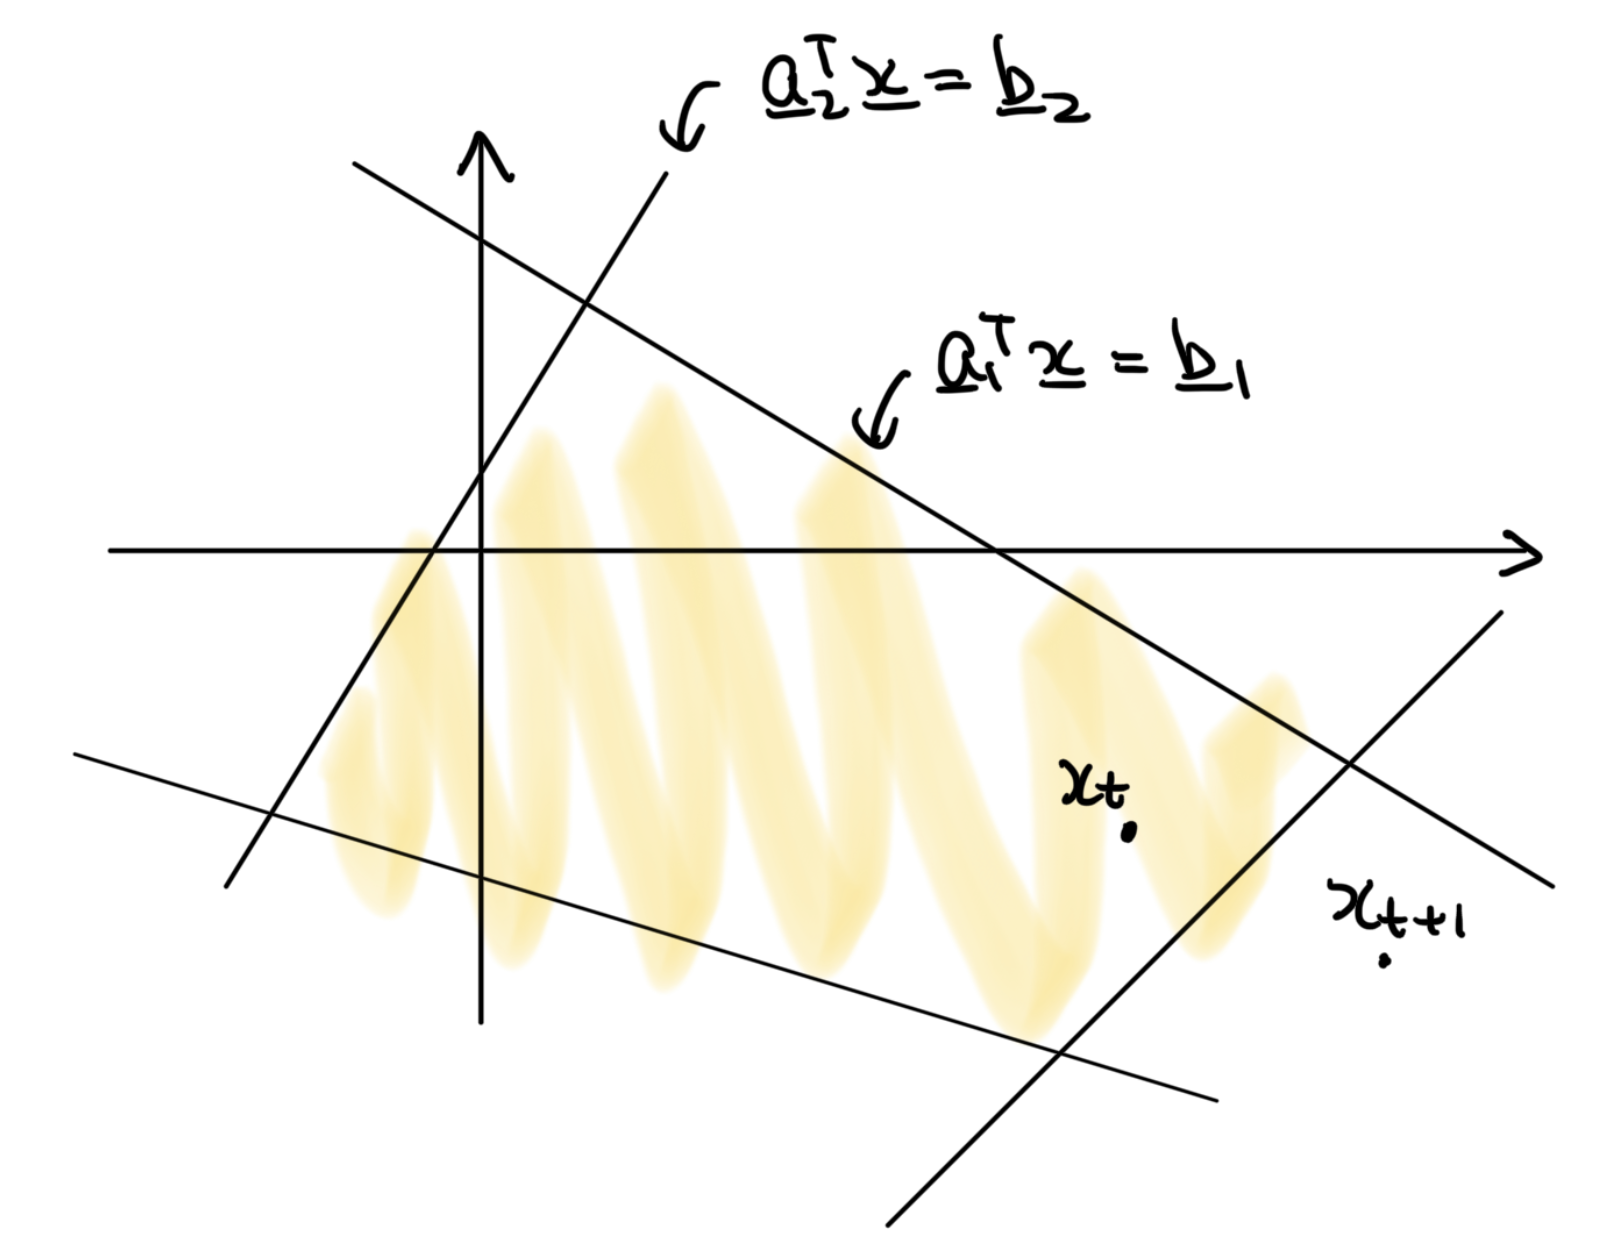
\includegraphics[width=0.70\linewidth]{fig/feasible-set.png}
    \caption{Feasible Set for Linear Constraints}
    \label{fig:feasible-set-linear-constraints}%
\end{figure}

Each constraint here gives a \(\pqty{n - 1}\)-dimensional linear subspace as the boundary (and hence the feasible set hence must be convex), as shown in \autoref{fig:feasible-set-linear-constraints}. Instead, we optimise in an unconstrained setup
\[
    \min_{\vb{x \in \RR^n}} \bqty{f\pqty{\vb{x}} + \sum_{i = 1}^{m} \phi\pqty{\vb{a}_i\transpose \vb{x} - \vb{b}_i}}
\]
where
\[
    \phi\pqty{x} = \begin{cases}
        x & \text{if } x \leq 0, \\ \plusinfty & \text{if } x > 0.
    \end{cases}
\]

Computationally, we apply a huge penalty on approaching the boundary, given by the function
\[
    \phi\pqty{x} = - \log \pqty{-x}
\]
for \(x < 0\). This is the \term{logarithmic barrier function}, as shown in \autoref{fig:barrier-function-comparison}.

\begin{figure}[ht!]
    \centering
    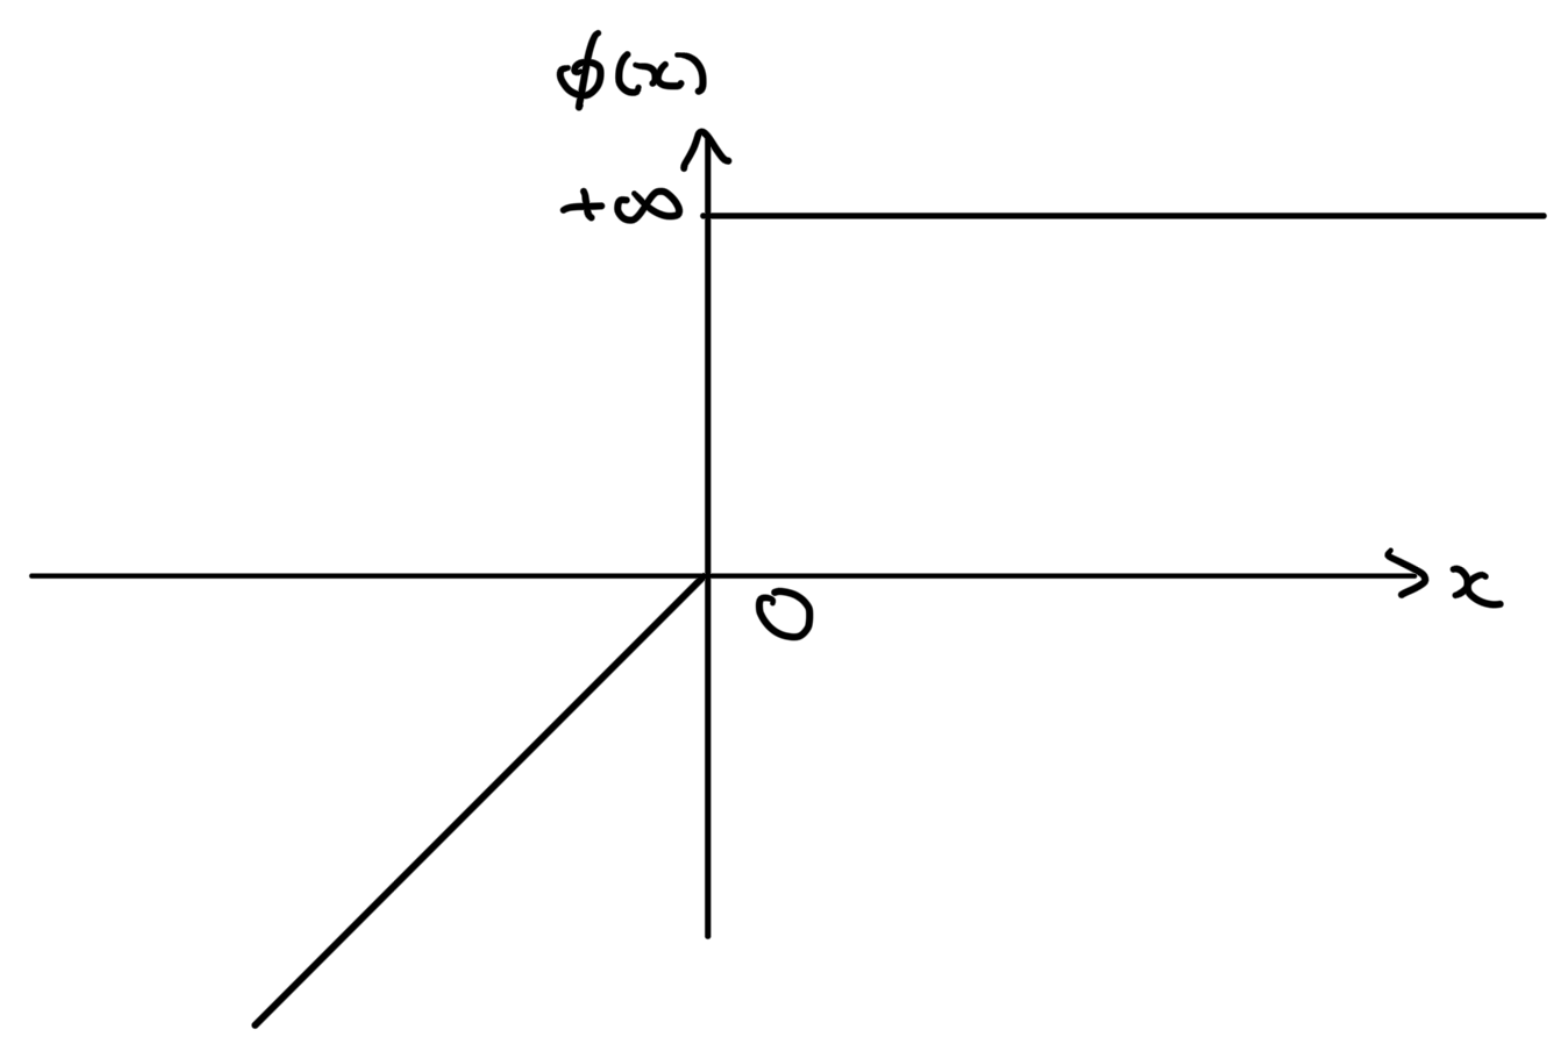
\includegraphics[width=0.7\linewidth]{fig/barrier-function-ideal.png}
    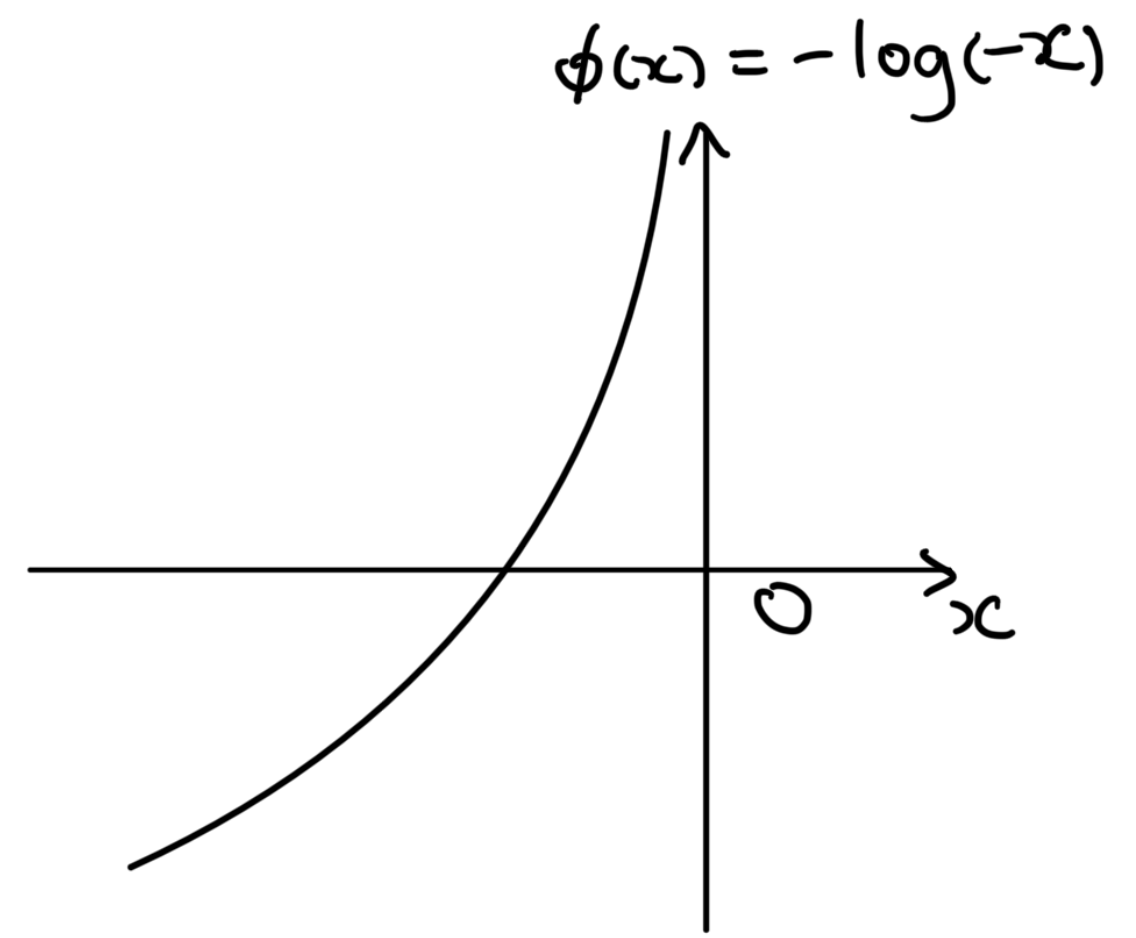
\includegraphics[width=0.5\linewidth]{fig/barrier-function-log.png}
    \caption{Barrier Function Comparison}
    \label{fig:barrier-function-comparison}%
\end{figure}

We introduce a parameter \(t > 0\), and the problem
\[
    \min_{\vb{x} \in \RR^n} \bqty{t f\pqty{\vb{x}} - \sum_{i = 1}^{m} \log\pqty{- \pqty{\vb{a}_i\transpose \vb{x} - \vb{b}_i}}}
\]
where \(t\) is a `balance' between the emphasis of the problem and the boundary. We repeatedly increase \(t\) and use gradient descent/Newton's method to optimise it. As \(t \to \plusinfty\), we approach the true minimum of the function \(f\pqty{\vb{x}}\). Formally, this is outlined in \autoref{alg:barrier-method}.

\begin{algorithm}[ht!]
    \caption{Barrier Method}\label{alg:barrier-method}%
    \begin{algorithmic}
        \Require \(f\) convex
        \Require \(\vb{x}\) strictly feasible
        \Require \(t > 0\)
        \Require \(\alpha > 1\)
        \Function{BarrierMethod}{\(f, \vb{x}, t, \alpha\)}
        \Repeat
            \State \(\vb{x}^{\ast} \pqty{t} \gets \argmin_{\vb{x} \in \RR^n} \bqty{t f\pqty{\vb{x}} - \sum_{i = 1}^{m} \log\pqty{- \pqty{\vb{a}_i\transpose \vb{x} - \vb{b}_i}}}\) using \textbf{Newton's Method} from \(\vb{x}\)
            \State \(\vb{x} \gets \vb{x}^{\ast} \pqty{t}\)
            \State \(t \gets \alpha t\)
        \Until{\(t\) is Sufficiently Large}
        \State \Return \(\vb{x}\)
        \EndFunction
    \end{algorithmic}
\end{algorithm}

The reason that we use Newton's algorithm is that the new optimum \(\vb{x}^{\ast} \pqty{\alpha t}\) is going to lie very close to \(\vb{x}^{\ast} \pqty{t}\), and Newton's method converges very rapidly to the new optimum.

This algorithm is used in solving linear programs as well (which we will see later -- another useful way is to use simplex algorithm). This, however, does not rely on the fact that linear optimums (for linear programs) are attained at vertices -- we just start on any interior point and use barrier method. But the number of vertices grow very quickly in higher dimensions, while barrier method allows us to solve it in linear time!
\section{Lagrange Multiplier Method}

We currently consider the constrained optimisation problem \(f\pqty{\vb{x}}\) subject to some constraint \(\vb{h}\pqty{\vb{x}} = \vb{b}\) with \(\vb{x} \in \mathcal{X}\) and \(\functiondomain{\vb{h}}{\RR^n}{\RR^m}\). There is no general algorithm to solve all constrained optimisation problems, but we may use a method called the \term{Lagrange multiplier method}.

\begin{definition}[Lagrangian, Lagrange Multiplier]
    We define the \term{Lagrangian} as
    \[
        L \pqty{\vb{x}, \vb*{\lambda}} = f\pqty{\vb{x}} - \vb*{\lambda}\transpose \pqty{\vb{h}\pqty{\vb{x}} - \vb{b}}
    \]
    where \(\vb*{\lambda} \in \RR^m\) is the \term{Lagrange multiplier}.
\end{definition}

We now minimise the Lagrangian, \(L\), simply in the region \(\vb{x} \in \mathcal{X}\), without worrying about the constraint.

\subsection{Lagrange Method}
\subsubsection{Lagrange Sufficiency}

\begin{theorem}[Lagrange Sufficiency]
    \label{thm:lagrange-sufficiency}%
    Let \(\vb{x}^{\ast} \in \mathcal{X}\) be such that \(\vb{h}\pqty{\vb{x}^{\ast}} = \vb{b}\), and \(\vb*{\lambda}^{\ast} \in \RR^m\), such that
    \[
        L\pqty{\vb{x}^{\ast}, \vb*{\lambda}^{\ast}} = \min_{\vb{x} \in \mathcal{X}} L\pqty{\vb{x}, \vb*{\lambda}^{\ast}}.
    \]

    Then \(\vb{x}^{\ast}\) also solves our original optimisation problem, i.e.,
    \[
        \min_{\vb{x} \in \mathcal{X} \pqty{\vb{b}}} f\pqty{\vb{x}} = f\pqty{\vb{x}^{\ast}}
    \]
\end{theorem}

\begin{proof}
    Suppose \(\pqty{\vb{x}^{\ast}, \vb*{\lambda}^{\ast}}\) is as stated in the theorem. Clearly,
    \[
        \min_{\vb{x} \in \mathcal{X} \pqty{\vb{b}}} f\pqty{\vb{x}} \leq f\pqty{\vb{x}^{\ast}}
    \]
    since \(\vb{x}^{\ast} \in \mathcal{X} \pqty{\vb{b}}\) is given.
    
    To prove the reverse inequality, we notice
    \begin{align*}
        \min_{\vb{x} \in \mathcal{X} \pqty{\vb{b}}} f\pqty{\vb{x}} &= \min_{\vb{x} \in \mathcal{X} \pqty{\vb{b}}} \bqty{f\pqty{\vb{x}} - {\vb*{\lambda}^{\ast}}\transpose \pqty{\vb{h} \pqty{\vb{x}} - \vb{b}}} \\
        &\geq \min_{\vb{x} \in \mathcal{X}} \bqty{f\pqty{\vb{x}} - {\vb*{\lambda}^{\ast}}\transpose \pqty{\vb{h} \pqty{\vb{x}} - \vb{b}}} \\
        &= f\pqty{\vb{x}^{\ast}} - {\vb*{\lambda}^{\ast}}\transpose \pqty{\vb{h} \pqty{\vb{x}^{\ast}} - \vb{b}} \\
        &= f\pqty{\vb{x}^{\ast}}.
    \end{align*}
\end{proof}

\begin{example}[Application of Lagrange Multiplier]
    We minimise the function \(- x_1 - x_2 + x_3\) subject to \(x_1^2 + x_2^2 = 4\), and \(x_1 + x_2 + x_3 = 1\).

    We construct the Lagrangian
    \begin{align*}
        L \pqty{\vb{x}, \vb*{\lambda}} &= L\pqty{x_1, x_2, x_3, \lambda_1, \lambda_2} \\
        &= - x_1 - x_2 + x_3 - \lambda_1 \pqty{x_1^2 + x_2^2 - 4} - \lambda_2 \pqty{x_1 + x_2 + x_3 - 1} \\
        &= \bqty{\pqty{-1 - \lambda_2} x_1 - \lambda_1 x_1^2} + \bqty{\pqty{-1 - \lambda_2} x_2 - \lambda_1 x_2^2} + \bqty{\pqty{1 - \lambda_2} x_3} + 4 \lambda_1 + \lambda_2.
    \end{align*}

    To minimise this with respect to \(x_1, x_2\) and \(x_3\) for general \(\vb*{\lambda}\), subject to no constraints, we must have \(\lambda_2 = 1\): otherwise there would be no minimum. Then, we have
    \[
        L = L\pqty{x_1, x_2, x_3, \lambda_1} = \pqty{-2 x_1 - \lambda_1 x_1^2} + \pqty{-2 x_2 - \lambda_1 x_2^2} + 4 \lambda_1 + 1.
    \]

    To have a finite minimum, we also need \(\lambda_1 < 0\), and the expression is optimised when
    \[
        x_1 = - \frac{1}{\lambda_1} \qand x_2 = - \frac{1}{\lambda_1}.
    \]

    Hence, the minimiser for \(\vb*{\lambda} = \pqty{\lambda_1, 1}\) would be
    \[
        \vb{x}^{\ast} = \pqty{- \frac{1}{\lambda_1}, - \frac{1}{\lambda_1}, x_3}
    \]
    for any \(x_3 \in \RR\).
    
    However, to apply \autoref{thm:lagrange-sufficiency}, we need to pick a value of \(\lambda_1\), such that the above \(\vb{x}^{\ast}\) is in fact feasible. We need to ensure that
    \[
        \frac{1}{\lambda_1^2} + \frac{1}{\lambda_1^2} = 4 \qand - \frac{1}{\lambda_1} - \frac{1}{\lambda_1} + x_3 = 1.
    \]

    This solves to \(\lambda_1 = - \flatfrac{1}{\sqrt{2}}\) (since \(\lambda_1 < 0\)) and \(x_3 = 1 - 2 \sqrt{2}\), giving
    \[
        \vb{x}^{\ast} = \pqty{\sqrt{2}, \sqrt{2}, 1 - 2 \sqrt{2}}
    \]
    with
    \[
        \vb*{\lambda}^{\ast} = \pqty{- \frac{1}{\sqrt{2}}, 1}.
    \]

    By \autoref{thm:lagrange-sufficiency} (Lagrange Sufficiency), we can now conclude that \(\vb{x}^{\ast}\) solves the original problem.
\end{example}

\subsubsection{Dual Feasibility}

\autoref{alg:lagrange-method} outlines the algorithm, with slack variables involved.

\begin{algorithm}[ht!]
    \caption{Lagrange Method with Slack Variables}\label{alg:lagrange-method}%
    \begin{algorithmic}
        \Function{LagrangeMethodSlackVariables}{\(\functiondomain{f}{\RR^n}{\RR}, \functiondomain{\vb{h}}{\RR^n}{\RR^m}, \vb{b} \in \RR^m, \mathcal{X} \subseteq \RR^n\)}
        
        \State \textbf{define} slack variables \(s_i \geq 0\) \textbf{and} rewrite the problem as \(\vb{h} \pqty{\vb{x}} + \vb{s} = \vb{b}\), for \(\vb{s} \geq \vb{0}\)

        \State \(L\pqty{\vb{x}, \vb{s}, \vb*{\lambda}} \gets f\pqty{\vb{x}} - \vb*{\lambda} \transpose \pqty{\vb{h}\pqty{\vb{x}} + \vb{s} - \vb{b}}\)

        \State \(\Lambda \gets \set{\vb*{\lambda} \in \RR^m}{\min_{\substack{\vb{x} \in \mathcal{X} \\ \vb{s} \geq \vb{0}}} L\pqty{\vb{x}, \vb{s}, \vb*{\lambda}} > \minusinfty}\)

        \For{\(\vb*{\lambda} \in \Lambda\)}
            \State \(\pqty{\vb{x}^{\ast} \pqty{\vb*{\lambda}}, \vb{s}^{\ast} \pqty{\vb*{\lambda}}} \gets \argmin_{\substack{\vb{x} \in \mathcal{X} \\ \vb{s} \geq \vb{0}}} L \pqty{\vb{x}, \vb{s}, \vb*{\lambda}}\)
        \EndFor

        \State \textbf{find} \(\vb*{\lambda}^{\ast} \in \Lambda\) \textbf{such that} \(\vb{h} \pqty{\vb{x}} + \vb{s} = \vb{b}\) \textbf{and} \(\vb{s} \geq \vb{0}\)

        \State \Return{\(\vb{x}^{\ast} \pqty{\vb*{\lambda}^{\ast}}\)}

        \EndFunction
    \end{algorithmic}
\end{algorithm}

\begin{definition}[Dual Feasible Set]
    The set
    \[
        \Lambda = \set{\vb*{\lambda} \in \RR^m}{\min_{\substack{\vb{x} \in \mathcal{X} \\ \vb{s} \geq \vb{0}}} L\pqty{\vb{x}, \vb{s}, \vb*{\lambda}} > \minusinfty}
    \]
    is the \term{dual feasible set}.
\end{definition}

\begin{proposition}[Complementary Slackness]
    For all \(\vb*{\lambda} \in \Lambda\) and their corresponding \(\vb{s}^{\ast} \pqty{\vb*{\lambda}}\), we have
    \begin{itemize}
        \item \(\vb*{\lambda} \leq \vb{0}\);
        \item \(\lambda_i s_i = 0\) (no summation convention): in particular, \(\lambda_i < 0\) implies \(s_i = 0\).
    \end{itemize}
\end{proposition}

\begin{proof}
    Notice that
    \[
        L\pqty{\vb{x}, \vb{s}, \vb*{\lambda}} = f\pqty{\vb{x}} - \vb*{\lambda} \transpose \pqty{\vb{h}\pqty{\vb{x}} - \vb{b}} - \vb*{\lambda}\transpose \vb{s},
    \]
    so we need \(\vb*{\lambda} \leq \vb{0}\), since otherwise we could just arbitrarily increase the corresponding component of \(\vb{s}\) to further decrease \(L\).

    Furthermore, if some particular \(\lambda_i < 0\), then we must have \(s_i = 0\) for the Lagrangian to be minimised. This implies that \(\lambda_i s_i = 0\).
\end{proof}

\begin{example}[Complementary Slackness]
    We minimise \(x_1 - 3 x_2\) subject to \(x_1^2 + x_2^2 \leq 4\) and \(x_1 + x_2 \leq 2\). We have
    \begin{align*}
        L\pqty{x_1, x_2, s_1, s_2, \lambda_1, \lambda_2} &= x_1 - 3 x_2 - \lambda_1 \pqty{x_1^2 + x_2^2 + s_1 - 4} - \lambda_2 \pqty{x_1 + x_2 + s_2 - 2} \\
        &= \pqty{\pqty{1 - \lambda_2} x_1 - \lambda_1 x_1^2} + \pqty{\pqty{-3 - \lambda_2} x_1 - \lambda_1 x_1^2} - \lambda_1 s_1 - \lambda_2 s_2 + 4 \lambda_1 + 2 \lambda_2.
    \end{align*}

    We consider the casework on whether \(\lambda_i < 0\) or \(\lambda_i = 0 \) (which gives four cases).

    \begin{enumerate}
        \item Suppose \(\lambda_1 = 0\). Then the first two quadratics will degenerate to linear equations, which cannot be both zero, and hence a minimum would not exist.
        \item Suppose \(\lambda_1 < 0, \lambda_2 < 0\). Then \(s_1 = s_2 = 0\), so
        \begin{align*}
            1 - 2 \lambda_1 x_1 - \lambda_2 &= 0, \\
            -3 - 2 \lambda_1 x_2 - \lambda_2 &= 0, \\
            x_1^2 + x_2^2 &= 4, \\
            x_1 + x_2 &= 2.
        \end{align*}

        From the final two equations, we have \(\pqty{x_1, x_2} = \pqty{2, 0}\) or \(\pqty{x_1, x_2} = \pqty{0, 2}\).
        
        If \(\pqty{x_1, x_2} = \pqty{0, 2}\), then we have \(\pqty{\lambda_1, \lambda_2} = \pqty{1, -3}\). If \(\pqty{x_1, x_2} = \pqty{2, 0}\), then we have \(\pqty{\lambda_1, \lambda_2} = \pqty{-1, 1}\). Neither solutions work.

        \item Suppose \(\lambda_1 < 0, \lambda_2 = 0\). Then \(s_1 = 0\), and hence
        \begin{align*}
            1 - 2 \lambda_1 x_1 &= 0, \\
            -3 - 2 \lambda_1 x_2 &= 0, \\
            x_1^2 + x_2^2 &= 4.
        \end{align*}

        Hence, we have
        \[
            x_1^{\ast} = \frac{1}{2 \lambda_1} \qand x_2^{\ast} = - \frac{3}{2 \lambda_1}
        \]
        and substituting to the final equation, we have \(\lambda_1 = - \sqrt{\flatfrac{5}{8}}\), giving us the optimal solution
        \[
            x_1^{\ast} = - \sqrt{\frac{2}{5}} \qand x_2^{\ast} = 3 \sqrt{\frac{2}{5}}.
        \]
    \end{enumerate}
\end{example}

\subsection{Weak and Strong Duality}

We consider our original problem, the \term{primal problem} without the slack variables, stated as minimising \(f\pqty{\vb{x}}\) subject to \(\vb{h}\pqty{\vb{x}} = \vb{b}\) and \(\vb{x} \in \mathcal{X}\).

\begin{definition}[Dual Objective Function, Dual Problem]
    The \term{dual objective function} \(\functiondomain{g}{\Lambda}{\RR}\) is defined as
    \[
        g\pqty{\vb*{\lambda}} = \min_{\vb{x} \in \mathcal{X}} L \pqty{\vb{x}, \vb*{\lambda}}
    \]
    where \(\Lambda\) is the dual feasible set.

    The \term{dual problem} is maximising \(g\pqty{\vb*{\lambda}}\) subject to \(\vb*{\lambda} \in \Lambda\).
\end{definition}

\begin{remark}
    The dual problem, theoretically, is much easier to solve than the primal problem. For every fixed \(\vb{x}\), the Lagrangian is linear in \(\vb*{\lambda}\), and the minimum of linear functions is concave.
\end{remark}

\begin{theorem}[Weak Duality]
    \label{weak-duality}%
    If \(\vb{x} \in \mathcal{X} \pqty{\vb{b}}\) is feasible, and \(\vb*{\lambda} \in \Lambda\), then
    \[
        f\pqty{\vb{x}} \geq g\pqty{\vb*{\lambda}}.
    \]

    In particular,
    \[
        \min_{\vb{x} \in \mathcal{X} \pqty{\vb{b}}} f\pqty{\vb{x}} \geq \max_{\vb*{\lambda} \in \Lambda} g\pqty{\vb*{\lambda}}.
    \]
\end{theorem}

\begin{proof}
    For any \(\vb*{\lambda} \in \Lambda\) and \(\vb{x} \in \mathcal{X}\pqty{\vb{b}}\), we have
    \begin{align*}
        f\pqty{\vb{x}} &\geq \min_{\vb{x} \in \mathcal{X} \pqty{\vb{b}}} f\pqty{\vb{x}} \\
        &= \min_{\vb{x} \in \mathcal{X} \pqty{\vb{b}}} \bqty{f\pqty{\vb{x}} - \vb*{\lambda} \transpose \pqty{\vb{h}\pqty{\vb{x}} - \vb{b}}} \\
        &\geq \min_{\vb{x} \in \mathcal{X}} \bqty{f\pqty{\vb{x}} - \vb*{\lambda} \transpose \pqty{\vb{h}\pqty{\vb{x}} - \vb{b}}} \\
        &= \min_{\vb{x} \in \mathcal{X}} L\pqty{\vb{x}, \vb*{\lambda}} \\
        &= g\pqty{\vb*{\lambda}}.
    \end{align*}
\end{proof}

\begin{definition}[Duality Gap, Strong Duality]
    We define the \textit{duality gap} as
    \[
        \min_{\vb{x} \in \mathcal{X} \pqty{\vb{b}}} f\pqty{\vb{x}} - \max_{\vb*{\lambda} \in \Lambda} g\pqty{\vb*{\lambda}}.
    \]

    If the duality gap is \(0\), then we say the problem satisfies the \term{strong duality} property.
\end{definition}

\begin{proposition}[Strong Duality is equivalent to Lagrange Method Working]
    The Lagrange method outlined in \autoref{thm:lagrange-sufficiency} works if and only if strong duality holds.
\end{proposition}

\begin{proof}
    Suppose the Lagrange method works. Then we have a pair \(\pqty{\vb{x}^{\ast}, \vb*{\lambda}^{\ast}}\) such that
    \[
        \argmin_{\vb{x} \in \mathcal{X}} L \pqty{\vb{x}, \vb*{\lambda}^{\ast}} = \vb{x}^{\ast}
    \]
    and \(\vb{h}\pqty{\vb{x}^{\ast}} = \vb{b}\). Then
    \begin{align*}
        g\pqty{\vb*{\lambda}^{\ast}} &= \min_{\vb{x} \in \mathcal{X}} \bqty{f\pqty{\vb{x}} - {\vb*{\lambda}^{\ast}}\transpose \pqty{\vb{h}\pqty{\vb{x}} - \vb{b}}} \\
        &= f\pqty{\vb{x}^{\ast}} - {\vb*{\lambda}^{\ast}}\transpose \pqty{\vb{h\pqty{\vb{x}^{\ast}}} - \vb{b}} \\
        &= f\pqty{\vb{x}^{\ast}}
    \end{align*}
    which gives a duality gap of zero.

    Suppose that strong duality holds, i.e., we can find \(\vb{x} \in \mathcal{X}\pqty{\vb{b}}\) and \(\vb*{\lambda} \in \Lambda\), such that \(f\pqty{\vb{x}} = g\pqty{\vb*{\lambda}}\). Then the Lagrange method works using this \(\vb*{\lambda}\) at this value of \(\vb{x}\) by definition of the dual objective problem.
\end{proof}

We now study how we may conclude strong duality (and hence when Lagrange method works).

\begin{definition}[Supporting Hyperplane]
    A function \(\functiondomain{\phi}{\RR^m}{\RR}\) is said to have a \term{supporting hyperplane} at a point \(\vb{b} \in \RR^m\), if there is some \(\vb*{\lambda} \in \RR^m\), such that for all \(\vb{c} \in \RR^m\), we have
    \[
        \phi\pqty{\vb{c}} \geq \phi\pqty{\vb{b}} + \vb*{\lambda}\transpose \pqty{\vb{c} - \vb{b}}.
    \]
\end{definition}

\begin{remarks}
    \begin{itemize}
        \item If \(\phi\) is differentiable at \(\vb{b}\), then the only possible choice is \(\vb*{\lambda} = \grad \phi \pqty{\vb{b}}\).
        \item If \(\phi\) is convex, then such supporting hyperplane always exists.
    \end{itemize}
\end{remarks}

\begin{definition}[Value Function]
    Define the \term{value function} \(\functiondomain{\phi}{\RR^m}{\RR}\) as
    \[
        \phi\pqty{\vb{c}} = \min_{\vb{x} \in \mathcal{X} \pqty{\vb{c}}} f\pqty{\vb{x}},
    \]
    where we recall the notation
    \[
        \mathcal{X} \pqty{\vb{c}} = \set{\vb{x} \in \mathcal{X}}{\vb{h}\pqty{\vb{x}} = \vb{c}}.
    \]
\end{definition}

\begin{theorem}[Strong Duality is equivalent to Existence of Supporting Hyperplane]
    Strong duality is satisfied if the value function \(\phi\) has a supporting hyperplane at \(\vb{b}\).

    Conversely, if strong duality holds for a suitable \(\vb*{\lambda}\), then \(\vb*{\lambda}\) is the supporting hyperplane to \(\phi\) at \(\vb{b}\).
\end{theorem}

\begin{proof}
    Suppose \(\phi\) has a supporting hyperplane \(\vb*{\lambda}\) at \(\vb{b}\). By definition,
    \[
        \phi\pqty{\vb{c}} \geq \phi\pqty{\vb{b}} + \vb*{\lambda}\transpose \pqty{\vb{c} - \vb{b}}.
    \]

    Then, we have
    \begin{align*}
        g\pqty{\vb*{\lambda}} &= \min_{\vb{x} \in \mathcal{X}} \bqty{f\pqty{\vb{x}} - \vb*{\lambda}\transpose \pqty{\vb{h}\pqty{\vb{x}} - \vb{b}}} \\
        &= \min_{\vb{c} \in \RR^m} \min_{\vb{x} \in \mathcal{X}\pqty{\vb{c}}} \bqty{f\pqty{\vb{x}} - \vb*{\lambda}\transpose \pqty{\vb{h}\pqty{\vb{x}} - \vb{c}} - \vb*{\lambda}\transpose \pqty{\vb{c} - \vb{b}}}.
    \end{align*}

    Now, note that
    \[
        \min_{\vb{x} \in \mathcal{X} \pqty{\vb{c}}} f\pqty{\vb{x}} = \phi\pqty{\vb{c}} \qand \forall \vb{x} \in \mathcal{X}\pqty{\vb{c}}: \vb{h}\pqty{\vb{x}} - \vb{c} = \vb{0},
    \]
    and hence
    \begin{align*}
         g\pqty{\vb*{\lambda}} &= \min_{\vb{c} \in \RR^m} \phi\pqty{\vb{c}} - \vb*{\lambda}\transpose \pqty{\vb{c} - \vb{b}} \\
         &\geq \phi\pqty{\vb{b}}
    \end{align*}
    by existence of supporting hyperplane. By weak duality, \(g\pqty{\vb*{\lambda}} \leq \phi\pqty{\vb{b}}\). Hence,
    \[
        g\pqty{\vb*{\lambda}} = \phi\pqty{\vb{b}}
    \]
    giving strong duality as desired.

    For the converse, if strong duality with that \(\vb*{\lambda}\), then
    \begin{align*}
        \phi\pqty{\vb{b}} &= g\pqty{\vb*{\lambda}} \\
        &= \min_{\vb{x} \in \mathcal{X}} \bqty{f\pqty{\vb{x}} - \vb*{\lambda}\transpose \pqty{\vb{h}\pqty{\vb{x}} - \vb{b}}} \\
        &= \min_{\vb{x} \in \mathcal{X}} \bqty{f\pqty{\vb{x}} - \vb*{\lambda}\transpose \pqty{\vb{h}\pqty{\vb{x}} - \vb{c}}} - \vb*{\lambda}\transpose \pqty{\vb{c} - \vb{b}} \\
        &\leq \min_{\vb{x} \in \mathcal{X}\pqty{\vb{c}}} \bqty{f\pqty{\vb{x}} - \vb*{\lambda}\transpose \pqty{\vb{h}\pqty{\vb{x}} - \vb{c}}} - \vb*{\lambda}\transpose \pqty{\vb{c} - \vb{b}} \\
        &= \phi\pqty{\vb{c}} - \vb*{\lambda}\transpose \pqty{\vb{c} - \vb{b}}
    \end{align*}
    showing the condition for the supporting hyperplane, as desired.
\end{proof}

For problems with inequality constraints stated as minimising \(f\pqty{\vb{x}}\) subject to \(\vb{h}\pqty{\vb{x}} \leq \vb{b}\) and \(\vb{x} \in \mathcal{X}\), the \term{value function} is defined similarly as
\[
    \phi\pqty{\vb{c}} = \min_{\vb{x} \in \mathcal{X} \pqty{\vb{c}}} f\pqty{\vb{x}}
\]
where instead
\[
    \mathcal{X} \pqty{\vb{c}} = \set{\vb{x} \in \mathcal{X}}{\vb{h}\pqty{\vb{x}} \leq \vb{c}}.
\]

\begin{theorem}[Sufficient Condition for Convexity of Value Function]
    If \(\mathcal{X}\) is a convex set, \(\functiondomain{f}{\RR^n}{\RR}\) is convex, and each component of \(\functiondomain{\vb{h}}{\RR^n}{\RR^m}\) is convex, then the value function for the optimisation problem with inequality constraints is convex.
\end{theorem}

\begin{proof}
    Consider \(\vb{c}\), \(\vb{c}'\) such that \(\mathcal{X} \pqty{\vb{c}}, \mathcal{X} \pqty{\vb{c}'} \neq \emptyset\). Let \(\vb{x} \in \mathcal{X}\pqty{\vb{c}}\), \(\vb{x}' \in \mathcal{X}\pqty{\vb{c}'}\), and \(t \in \ccintv{0}{!}\). Then \(t \vb{x} + \pqty{1 - t} \vb{x}' \in \mathcal{X}\) by convexity of \(\mathcal{X}\). Note that by convexity of \(h_j\), we have
    \begin{align*}
        h_j\pqty{t \vb{x} + \pqty{1 - t} \vb{x}'} &\leq t h_j\pqty{\vb{x}} + \pqty{1 - t} h_j\pqty{\vb{x}'} \\
        &\leq t c_j + \pqty{1 - t} c_j'
    \end{align*}
    so
    \[
        t \vb{x} + \pqty{1 - t} \vb{x}' \in \mathcal{X} \pqty{t \vb{c} + \pqty{1 - t} \vb{c}'}.
    \]

    We hence have (by convexity of \(f\))
    \begin{align*}
        \phi\pqty{t \vb{c} + \pqty{1 - t} \vb{c}'} &\leq f\pqty{t \vb{x} + \pqty{1 - t} \vb{x}'} \\
        &\leq t f\pqty{\vb{x}} + \pqty{1 - t} f\pqty{\vb{x}'}
    \end{align*}
    for all \(\vb{x} \in \mathcal{X}\pqty{\vb{c}}\), \(\vb{x}' \in \mathcal{X}\pqty{\vb{c}'}\). Taking the minimum over all \(\vb{x}\) and \(\vb{x}'\) gives
    \[
        \phi\pqty{t \vb{c} + \pqty{1 - t} \vb{c}'} \leq t \phi\pqty{\vb{c}} + \pqty{1 - t} \phi\pqty{\vb{c}'}
    \]
    as desired.
\end{proof}

Note \(\vb{h}\pqty{\vb{x}} = \vb{b}\) is equivalent to \(\vb{h}\pqty{\vb{x}} \leq \vb{b}\) and \(- \vb{h}\pqty{\vb{x}} \leq - \vb{b}\), so the above theorem also applies to equality constraints, if \(\vb{h}\) and \(-\vb{h}\) are both convex, i.e., \(\vb{h}\) is linear.
\section{Linear Program and Simplex Algorithm}

We restrict ourselves to an even more special type of constrained optimisation, where we not only require the functions/regions to be \emph{convex}, but furthermore \textbf{linear}.

\begin{definition}[Linear Program]
    A \term{linear program} is a constrained optimisation problem where we \textbf{minimise} \(\vb{c}\transpose \vb{x}\), subject to \textbf{constraints} of the form
    \begin{itemize}
        \item \(\vb{a}_i\transpose \vb{x} \geq b_i\), for all \(i \in M_1\),
        \item \(\vb{a}_i\transpose \vb{x} \leq b_i\), for all \(i \in M_2\),
        \item \(\vb{a}_i\transpose \vb{x} = b_i\), for all \(i \in M_3\),
        \item \(x_j \geq 0\), for all \(j \in N_1\),
        \item \(x_j \leq 0\), for all \(j \in N_2\),
        \item \(x_j \in \RR\), for all \(j \in N_3\).
    \end{itemize}

    We denote \(m = \abs{M_1} + \abs{M_2} + \abs{M_3}\) as the \textbf{number of constraints}, and \(n = \abs{N_1} + \abs{N_2} + \abs{N_3}\) as the \textbf{dimension}.
\end{definition}

We may put the constraint vectors into a matrix
\[
    \vb{A} = \pmqty{
        \text{---} & \vb{a}_1\transpose & \text{---} \\
        \text{---} & \vb{a}_2\transpose & \text{---} \\
         & \vdots & \\
        \text{---} & \vb{a}_m\transpose & \text{---}
    }
\]
and we denote its columns as \(\vb{A}_1, \vb{A}_2, \ldots, \vb{A}_n\).

\subsection{Duality of Linear Programs}

\subsubsection{Dual Form of a Linear Program}

\begin{theorem}[Dual Form of a Linear Program]
    The dual of the linear program defined above is given by maximising \(\vb{b}\transpose \vb*{\lambda}\), subject to the constraints
    \begin{itemize}
        \item \(\lambda_i \geq 0\) for all \(i \in M_1\),
        \item \(\lambda_i \leq 0\) for all \(i \in M_2\),
        \item \(\lambda_i \in \RR\) for all \(i \in M_3\),
        \item \(\vb*{\lambda}\transpose \vb{A}_j \leq c_j\) for all \(j \in N_1\),
        \item \(\vb*{\lambda}\transpose \vb{A}_j \geq c_j\) for all \(j \in N_2\),
        \item \(\vb*{\lambda}\transpose \vb{A}_j = c_j\) for all \(j \in N_3\).
    \end{itemize}
\end{theorem}

\begin{proof}
    Adding slack variables to get rid of the inequality constraints to transform the constraints to the form
    \[
        \forall i \in M_1: \vb{a}_i\transpose \vb{x} - s_i = b_i \qand \forall i \in M_2: \vb{a}_i\transpose \vb{x} + s_i = b_i,
    \]
    the Lagrangian \(L\pqty{\vb{x}, \vb{s}, \vb*{\lambda}}\) satisfies
    \begin{align*}
        L\pqty{\vb{x}, \vb{s}, \vb*{\lambda}} &= \vb{c}\transpose \vb{x} - \sum_{i \in M_1} \lambda_i \pqty{\vb{a}_i\transpose \vb{x} - s_i - b_i} - \sum_{i \in M_2} \lambda_i \pqty{\vb{a}_i\transpose \vb{x} + s_i - b_i} - \sum_{i \in M_3} \lambda_i \pqty{\vb{a}_i\transpose \vb{x} - b_i} \\
        &= \sum_{j \in N_1} \pqty{c_j - \vb*{\lambda}\transpose \vb{A}_j} x_j + \sum_{j \in N_2} \pqty{c_j - \vb*{\lambda}\transpose \vb{A}_j} x_j + \sum_{j \in N_3} \pqty{c_j - \vb*{\lambda}\transpose \vb{A}_j} x_j \\
        &\phantom{=} \hspace{13em} + \sum_{i \in M_1} \lambda_i s_i - \sum_{i \in M_2} \lambda_i s_i + \sum_{i \in M_1 \cup M_2 \cup M_3} \lambda_i b_i.
    \end{align*}

    We observe that
    \[
        \Lambda = \set{\vb*{\lambda} \in \RR^m}{\begin{aligned}
            \forall i \in M_1 & : \lambda_i \geq 0 \\
            \forall i \in M_2 & : \lambda_i \leq 0 \\
            \forall i \in M_3 & : \lambda_i \in \RR \\
            \forall j \in N_1 & : \vb*{\lambda}\transpose \vb{A}_j \leq c_j \\
            \forall j \in N_2 & : \vb*{\lambda}\transpose \vb{A}_j \geq c_j \\
            \forall j \in N_3 & : \vb*{\lambda}\transpose \vb{A}_j = c_j
        \end{aligned}},
    \]

    If \(\vb*{\lambda} \in \Lambda\), then by simply setting all the previous terms to zero, we have
    \[
        g\pqty{\vb*{\lambda}} = \min_{\substack{\vb{x} \in \mathcal{X} \\ \vb{s} \geq 0}} L\pqty{\vb{x}, \vb{s}, \vb*{\lambda}} = \vb{b}\transpose \vb*{\lambda}.
    \]
\end{proof}

\subsubsection{Optimality Conditions}

\begin{theorem}[Optimality Conditions for Linear Programs]
    \label{thm:optimality-condition-lp}%
    Let \(\vb{x}\) and \(\vb*{\lambda}\) be feasible solutions to the primal linear program and its dual. Then these are optimal if and only if
    \[
        \lambda_i \pqty{\vb{a}_i \transpose \vb{x} - b_i} = 0 \qand \pqty{c_j - \vb*{\lambda}\transpose \vb{A}_j} x_j = 0
    \]
    for all \(i\) and \(j\).
\end{theorem}

\begin{proof}
    Define \(u_i = \lambda_i \pqty{\vb{a}_i \transpose \vb{x} - b_i}\) and \(v_j = \pqty{c_j - \vb*{\lambda}\transpose \vb{A}_j} x_j\). Since \(\vb{x}\) and \(\vb*{\lambda}\) are both feasible, we have \(u_i \geq 0\) and \(v_j \geq 0\) for all \(i\) and \(j\).

    Summing up with respect to \(i\) and \(j\) respectively, we have
    \[
        \sum_{i \in M_1 \cup M_2 \cup M_3} u_i = \vb*{\lambda}\transpose \vb{A} \vb{x} - \vb*{\lambda}\transpose \vb{b}
    \]
    and
    \[
        \sum_{j \in N_1 \cup N_2 \cup N_3} v_j = \vb{c}\transpose \vb{x} - \vb*{\lambda}\transpose \vb{A} \vb{x}.
    \]

    Hence,
    \[
        \sum_{i \in M_1 \cup M_2 \cup M_3} u_i + \sum_{j \in N_1 \cup N_2 \cup N_3} v_j = \vb{c}\transpose \vb{x} - \vb*{\lambda}\transpose \vb{b}.
    \]

    But by weak duality, we know that \(\vb{c}\transpose \vb{x} \geq \vb*{\lambda}\transpose \vb{b}\).

    If \(\vb{c}\transpose \vb{x} = \vb*{\lambda}\transpose \vb{b}\) (i.e. \(\vb{x}\) and \(\vb*{\lambda}\) are optimal), then \(u_i = 0\) and \(v_j = 0\) for all \(i\) and \(j\).

    Conversely, if \(u_i = 0\) and \(v_j = 0\) for all \(i\) and \(j\), then \(\vb{c}\transpose \vb{x} = \vb*{\lambda}\transpose \vb{b}\), and hence \(\vb{x}\) and \(\vb*{\lambda}\) are optimal by weak duality.
\end{proof}

\subsection{Standard and General Forms of Linear Programs}

We may always convert any linear program into its \term{general form} by flipping signs, splitting equalities into two inequalities, and converting the sign constraints also into scalar product constraints as well.

\begin{definition}[General Form of a Linear Program]
    The \term{general form} of a linear program is a linear program re-written as \textbf{minimising} \(\vb{c}\transpose \vb{x}\) subject to a constraint \(\vb{A}\vb{x} \leq \vb{b}\).
\end{definition}

\begin{definition}[Standard Form of a Linear Program]
    The \term{standard form} of a linear program is a linear program re-written as \textbf{minimising} \(\vb{c}\transpose \vb{x}\) subject to a constraint \(\vb{A}\vb{x} = \vb{b}\) and \(\vb{x} \geq 0\).
\end{definition}

Clearly, all standard form linear programs can be converted into general form. To convert linear programs in general form to standard form, we first add slack variables to convert it to optimise \(\vb{c}\transpose \vb{x}\), subject to \(\vb{A} \vb{x} + \vb{s} = \vb{b}\), with \(\vb{s} \geq \vb{0}\).

A further trick to convert from general form to special form is to write
\[
    x_j = x_j^+ - x_j^-
\]
where \(x_j\) is any real number, while \(x_j^+\) and \(x_j^-\) are non-negative real numbers. This allows us to convert the previous form to optimise \(\vb{c}\transpose \pqty{\vb{x}_+ - \vb{x}_-}\), subject to \(\vb{A} \pqty{\vb{x}_+ - \vb{x}_-} + \vb{s} = \vb{b}\), with \(\vb{x}_+, \vb{x}_-, \vb{s} \geq \vb{0}\).

In practice, it is often easier to discuss the \emph{theory} in general form, while the \emph{algorithms} are often discussed in standard form.

\subsection{Extreme Points and Basic Feasible Solutions}
\subsubsection{Maximising Convex Functions}

Minimising \(\vb{c}\transpose \vb{x}\) is the same as maximising \(-\vb{c}\transpose \vb{x}\), which must be a convex function. We are essentially trying to \emph{maximise} a convex function. (Previously we attempted to \emph{minimise} a convex function instead.) Intuitively, it must lie somewhere along the ``boundary'' of a set, but this is not the boundary simply in the topological sense, since it cannot be on a straight ``edge'' as well.

\begin{definition}[Extreme Point in Convex Set]
    A point \(\vb{x} \in C\) where \(C \subseteq \RR^n\) is convex, is called an \term{extreme point}, if it \emph{cannot} be written as a convex combination of two distinct points in \(C\), i.e., for \(\vb{y}, \vb{z} \in C\) and \(\delta \in \oointv{0}{1}\),
    \[
        \vb{x} = \delta \vb{y} + \pqty{1 - \delta} \vb{z} \implies \vb{x} = \vb{y} = \vb{z}.
    \]
\end{definition}

In other words, an extreme point in a convex set does not lie on a line segment (strictly) between two points.

\begin{proposition}[Maximum of a Convex Function occurs at Extreme Points]
    The maximum of a convex function \(\functiondomain{f}{C}{\RR}\) occurs at an extreme point of \(C\).
\end{proposition}

\begin{proof}
    Suppose \(\vb{x}\) maximise \(f\) and is not an extreme point. Then
    \[
        \vb{x} = \delta \vb{y} + \pqty{1 - \delta} \vb{z}
    \]
    for some \(\vb{y}, \vb{z} \in C\) and \(\delta \in \oointv{0}{1}\), with \(\vb{y} \neq \vb{z}\). But by convexity,
    \[
        f\pqty{\vb{x}} \leq \delta f\pqty{\vb{y}} + \pqty{1 - \delta} f\pqty{\vb{z}} \leq \max \Bqty{f\pqty{\vb{y}}, f\pqty{\vb{z}}}
    \]
    so it has to maximise at one of the ends of the line segment as well.
\end{proof}

\begin{figure}[ht!]
    \centering
    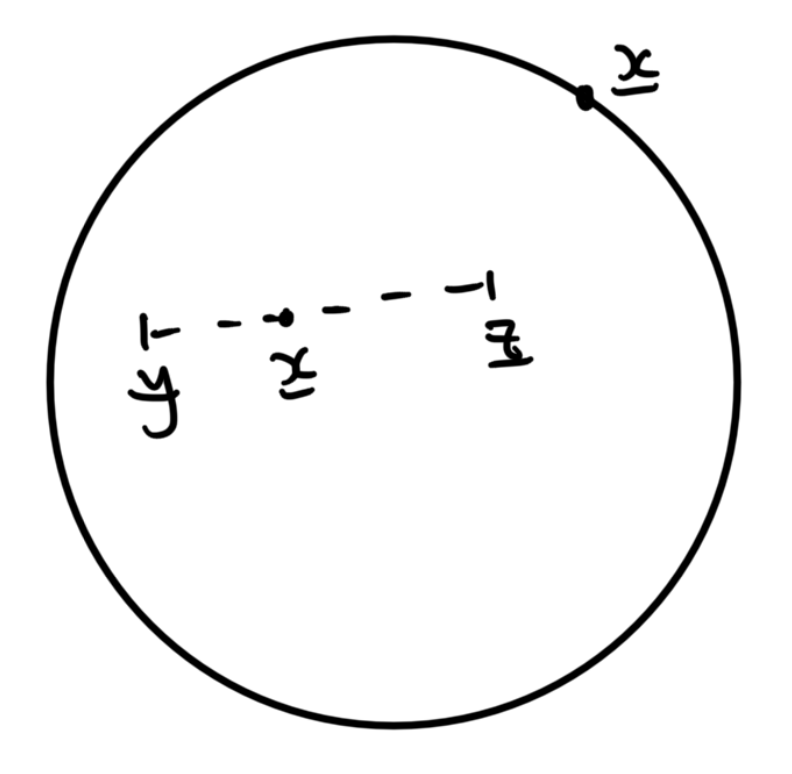
\includegraphics[width=0.3\linewidth]{fig/circle-extreme-points.png}
    \caption{Extreme Point of a Circle}
    \label{fig:circle-extreme-point}
\end{figure}

\begin{figure}[ht!]
    \centering
    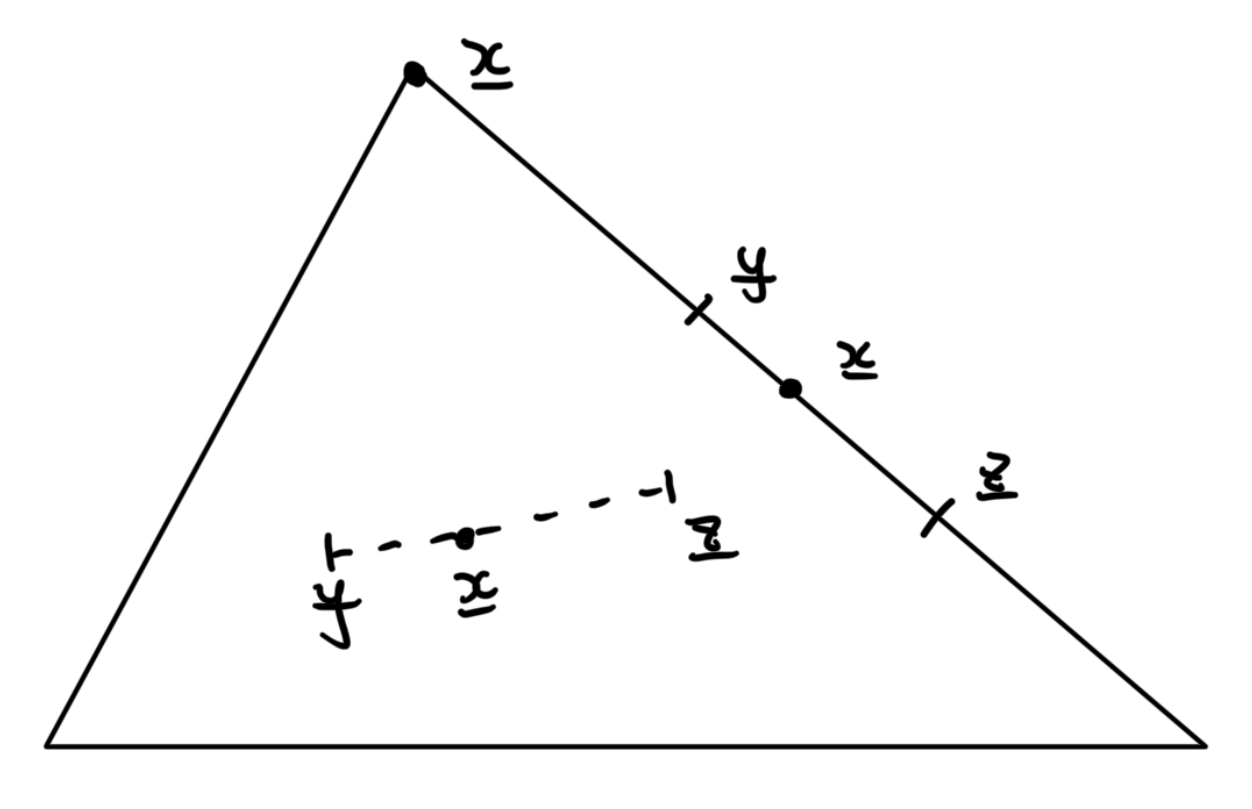
\includegraphics[width=0.5\linewidth]{fig/triangle-extreme-points.png}
    \caption{Extreme Point of a Triangle}
    \label{fig:triangle-extreme-point}
\end{figure}

A convex set may have infinitely many extreme points (such as a circle, in \autoref{fig:circle-extreme-point}), which does not really help. In linear programs, since the constraints are linear, the regions are (higher-dimensional) polygons, which means the extreme points are in fact finite (for example, in \autoref{fig:triangle-extreme-point} for a triangle) -- so now it suffices for us to have a list of extreme points for linear constraints.

\subsubsection{Basic Solutions and Basic Feasible Solutions}

We now look at a linear program in standard form, where the constraint is given by \(\vb{A} \vb{x} = \vb{b}\), where the matrix \(\vb{A} \in \RR^{m \times n}\) have rows \(\vb{a}_1\transpose, \vb{a}_2\transpose, \ldots, \vb{a}_m\transpose\), and columns \(\vb{A}_1, \vb{A}_2, \ldots, \vb{A}_n\).

We will be making three assumptions, the first two of which are stated below.

\begin{enumerate}[label=(\Alph*)]
    \item Without loss of generality, rows of \(\vb{A}\) are linearly independent. (This would remove the duplications of a constraint.)
    \item \textbf{Every} set of \(m\) columns of \(\vb{A}\) is linearly independent. (This assumption \textbf{cannot} be made without loss of generality.)
\end{enumerate}

The third requires some other definition.

\begin{definition}[Basic Solution, Basic Feasible Solution]
    A point \(\vb{x} \in \RR^n\) that satisfies \(\vb{Ax} = \vb{b}\) and has at most \(m\) non-zero entries is called a \term{basic solution}. A basic solution \(\vb{x}\) that satisfies \(\vb{x} \geq \vb{0}\) is called a \term{basic feasible solution}.
\end{definition}

To construct basic solutions, we notice that the system \(\vb{Ax} = \vb{b}\) is underdetermined, since \(n > m\).

Suppose we choose indices \(\Bqty{\basis\pqty{1}, \basis\pqty{2}, \ldots, \basis\pqty{m}}\) such that \(x_i = 0\) for all \(i \notin \Bqty{\basis\pqty{1}, \basis\pqty{2}, \ldots, \basis\pqty{m}}\). Notice that
\[
    \vb{Ax} = \sum_{i = 1}^{n} \vb{A}_i x_i = \sum_{i = 1}^{m} \vb{A}_{\basis\pqty{i}} x_{\basis\pqty{i}}.
\]

This essentially makes solving the original system equivalent to solving a new system
\[
    \vb{B} \vb{x}_{\basis} = \vb{b}
\]
where the new matrix \(\vb{B}\) is defined as
\[
    \vb{B} = \pmqty{
        | & | & \cdots & | \\
        \vb{A}_{\basis\pqty{1}} & \vb{A}_{\basis\pqty{2}} & \cdots & \vb{A}_{\basis\pqty{m}} \\
        | & | & \cdots & |
    }
\]
and the new vector \(\vb{x}_{\basis}\) is defined as
\[
    \vb{x}_{\basis} = \pmqty{
        x_{\basis\pqty{1}} \\
        x_{\basis\pqty{2}} \\
        \vdots \\
        x_{\basis\pqty{n}}
    }.
\]

\begin{definition}[Basic Matrix, Basic Variables]
    We fix a choice of \(\basis\). The variables \(x_{\basis\pqty{1}}, x_{\basis\pqty{2}}, \ldots, x_{\basis\pqty{m}}\) are the \term{basic variables}. The matrix \(\vb{B}\) is the \term{basic matrix}, and its columns, \(\vb{A}_{\basis\pqty{1}}, \vb{A}_{\basis\pqty{2}}, \ldots, \vb{A}_{\basis\pqty{m}}\), are the \term{basic columns}.
\end{definition}

For every choice of \(\basis\) (there are \(\binom{n}{m}\) of those), we get a basic solution. Furthermore, if \(\vb{x}_{\basis} = \vb{B}\inverse \vb{b} \geq \vb{0}\), then that basis \(\vb{B}\) leads to a basic feasible solution.

We now state the final assumption.

\begin{enumerate}[resume*]
    \item \textbf{Every} basic feasible solution is ``non-degenerate'', that is, it has exactly \(m\) non-zero entries. (This means we want the inequality to be strict: \(\vb{B}\inverse \vb{b} \geq \vb{0} \implies \vb{B}\inverse \vb{b} > \vb{0}\).)
\end{enumerate}

\subsubsection{Equivalence between Extreme Points and Basic Feasible Solutions}

\begin{theorem}[Extreme Points of Feasible Set are precisely Basic Feasible Solutions]
    A vector \(\vb{x}\) is a basic feasible solution, if and only if it is an extreme point of the set
    \[
        \mathcal{X} \pqty{\vb{b}} = \set{\vb{x} \in \RR^n}{\vb{Ax} = \vb{b}, \vb{x} \geq 0}.
    \]
\end{theorem}

\begin{remark}
    Bad algorithms to solve linear programs could be:
    \begin{itemize}
        \item list all \(\binom{n}{m}\) basic solutions;
        \item filter out basic feasible solutions (BFS) from this list;
        \item evaluate \(\vb{c}\transpose \vb{x}\) for each BFS and choose the best one.
    \end{itemize}

    But even if \(m \approx \flatfrac{n}{2}\), then the time taken would grow exponentially.
\end{remark}

\begin{proof}
    Suppose \(\vb{x}\) is a basic feasible solution that can be written as
    \[
        \vb{x} = \pqty{1 - \delta} \vb{y} + \delta \vb{z}
    \]
    for \(\vb{y}, \vb{z} \in \mathcal{X} \pqty{\vb{b}}\) and \(\delta \in \oointv{0}{1}\).

    If \(x_i = 0\), then \(y_i = z_i = 0\) since \(\delta \in \oointv{0}{1}\) and \(y_i, z_i \geq 0\).

    Since \(\vb{x}\) is a basic feasible solution, \(\vb{y}\) and \(\vb{z}\) must be basic solutions corresponding to the same basis as \(\vb{x}\). This therefore implies \(\vb{x} = \vb{y} = \vb{z}\).

    Now instead, we suppose \(\vb{x}\) is \textbf{not} a basic feasible solution. If \(\vb{x} \notin \mathcal{X} \pqty{\vb{b}}\), then obviously it is not an extreme point of \(\mathcal{X} \pqty{\vb{b}}\), so we consider that \(\vb{x} \in \mathcal{X} \pqty{\vb{b}}\), i.e., \(\vb{x}\) is feasible.

    Because \(\vb{x}\) is not a basic feasible solutions, it must have at least \(r > m\) possible entries.
    
    Suppose \(x_{i_1}, x_{i_2}, \ldots, x_{i_r} > 0\), then the columns \(\vb{A}_{i_1}, \vb{A}_{i_2}, \ldots, \vb{A}_{i_r}\) are linearly dependent, since \(r > m\). Let a non-trivial zero linear combination be
    \[
        w_{i_1} \vb{A}_{i_1} + w_{i_2} \vb{A}_{i_2} + \cdots + w_{i_r} \vb{A}_{i_r} = \vb{0}.
    \]

    Construct a vector \(\vb{w}\) such that it has components zero, except at locations \(i_1\), \(i_2\), \(\ldots\), \(i_r\) where we set its components to the coefficients in the linear combination above. Observe that \(\vb{Aw} = \vb{0}\). Now consider two new points
    \[
        \vb{y} = \vb{x} + \epsilon \vb{w} \qand \vb{z} = \vb{x} - \epsilon \vb{w}
    \]
    where \(0 < \epsilon \ll 1\) is sufficiently small.
    
    We claim \(\vb{y}\) and \(\vb{z}\) are feasible. The only possible reason why they would fail to be feasible is if accidentally one of the coordinates become negative, but since we are only adjusting the indices that are strictly greater than zero, taking \(\epsilon\) sufficiently small will prevent this from happening.

    This means
    \[
        \vb{x} = \frac{1}{2} \vb{y} + \frac{1}{2} \vb{z},
    \]
    which means that \(\vb{x}\) cannot be an extreme point.
\end{proof}

\subsection{Simplex Method}
\subsubsection{Towards the Simplex Method}

When the linear program is in standard form, the optimality conditions are:
\begin{enumerate}
    \item Primal feasibility: \(\vb{Ax} = \vb{b}\), \(\vb{x} \geq 0\),
    \item Dual feasibility: \(\vb{A}\transpose \vb*{\lambda} \leq \vb{c}\), and
    \item Complementary Slackness: \(\vb{x}\transpose \pqty{\vb{c} - \vb{A}\transpose \vb*{\lambda}} = 0\).
\end{enumerate}

For any basic feasible solution, the complementary slackness equation reduces to
\[
    \vb{x}_{\basis}\transpose \pqty{\vb{c}_{\basis} - \vb{B}\transpose \vb*{\lambda}} = 0
\]
due to the non-zero components in \(\vb{x}\). But since \(\vb{x}_{\basis} > \vb{0}\) (due to non-degeneracy assumption), we need
\[
    \vb{c}_{\basis} = \vb{B}\transpose \vb*{\lambda}.
\]  

This means
\[
    \vb*{\lambda} = \pqty{\vb{B}\transpose}\inverse \vb{c}_{\basis}.
\]

Therefore, if
\[
    \boxed{\vb{A}\transpose \pqty{\vb{B}\transpose}\inverse \vb{c}_{\basis} \leq \vb{c}}
\]
then \(\vb*{\lambda}\) is dual feasible, hence \(\vb{x}\) is optimal. This gives us a way of checking optimality simply using the choice of \(\basis\) and checking the above inequalities.

\begin{definition}[Reduced Costs Vector]
    We define the \term{vector of reduced costs} as a row vector
    \[
        \bar{\vb{c}}\transpose = \vb{c}\transpose - \vb{c}_{\basis}
        \transpose \vb{B}\inverse \vb{A}.
    \]
\end{definition}

With this new notation, the above derivation can be summarised into the following theorem.

\begin{theorem}[Reduced Costs Vector being Non-Negative implies Optimality]
    If for some basic feasible solution \(\vb{x}\) we have \(\bar{\vb{c}} \geq \vb{0}\), then such solution \(\vb{x}\) must be optimal.
\end{theorem}

\subsubsection{Outlining the Simplex Algorithm}

Suppose we have a basic feasible solution
\[
    \vb{x} = \pmqty{
        x_{\basis\pqty{1}} \\
        x_{\basis\pqty{2}} \\
        \vdots \\
        x_{\basis\pqty{m}} \\
        0 \\
        \vdots \\
        0}.
\]

Suppose, for some \(j^{\ast}\), we have \(\bar{c}_{j^{\ast}} < 0\) (i.e., this solution is not optimal). Suppose we choose some
\[
    j \notin \Bqty{\basis\pqty{1}, \ldots, \basis\pqty{m}}
\]
and we decide to make \(x_j > 0\), while keeping all non-basic \(x_i\)s still be zero. Then after this perturbation, the new vector would look like
\[
   \pmqty{
        x_{\basis\pqty{1}} \\
        x_{\basis\pqty{2}} \\
        \vdots \\
        x_{\basis\pqty{m}} \\
        0 \\
        \vdots \\
        0 \\
        0 \\ 
        0 \\
        \ldots \\
        0}
    + t \pmqty{
        d_{\basis\pqty{1}} \\
        d_{\basis\pqty{2}} \\
        \vdots \\
        d_{\basis\pqty{m}} \\
        0 \\
        \vdots \\
        0 \\
        1 \\
        0 \\
        \vdots \\
        0}
\]
where \(t > 0\). We want \(\vb{Ax} = \vb{b}\) still to be satisfied (for it still be feasible), i.e.,
\[
    \vb{A} \pmqty{\vb{d}_{\basis} \\ 0 \\ \vdots \\ 0 \\ 1 \\ 0 \\ \vdots \\ 0} = \vb{0}.
\]

This is equivalent to saying
\[
    \vb{B} \vb{d}_{\basis} + \vb{A}_j = 0
\]
and the direction we want to move in is
\[
    \vb{d}_{\basis} = - \vb{B}\inverse \vb{A}_j
\]

We now look at the new cost at the perturbed point. We have
\begin{align*}
    \vb{c}\transpose \pqty{\vb{x} + t \pmqty{\vb{d}_{\basis} \\ 0 \\ \vdots \\ 0 \\ 1 \\ 0 \\ \vdots \\ 0}} &= \vb{c}\transpose \vb{x} + t \pqty{\vb{c}_{\basis}\transpose \vb{d}_{\basis} + c_j} \\
    &= \vb{c}\transpose \vb{x} + t \pqty{c_j - \vb{c}_{\basis}\transpose \vb{B}\inverse \vb{A}_j} \\
    &= \vb{c}\transpose \vb{x} + t \bar{c}_j
\end{align*}

To ensure the new \(\vb{x}\) is still feasible, we can calculate
\[
    - \frac{x_{\basis \pqty{1}}}{d_{\basis \pqty{1}}}, \ldots, - \frac{x_{\basis \pqty{m}}}{d_{\basis \pqty{m}}},
\]
and find the smallest positive number out of those. Say, if \(d_{\basis\pqty{j}} < 0\), then \(x_{\basis\pqty{j}}\) could become negative if \(t\) is too big. Therefore, we let \(t\) to be the smallest positive number. Call this \(t^{\ast}\). Then the new point \(\vb{y}\), defined as
\[
    \vb{y} = \vb{x} + t^{\ast} \vb{d},
\]
is in fact a basic feasible solution: we have \(\vb{Ay} = \vb{b}\) and \(\vb{y} \geq \vb{0}\) (so it is feasible), and it has exactly \(m = \pqty{m - 1} + 1\) non-zero entries, since the value \(t^{\ast}\) ensures exactly one of the \(m\) basic entries \(y_{\basis\pqty{1}}, \ldots, y_{\basis\pqty{m}}\) becomes zero, while the entering index is still non-zero. \(\vb{y}\) is guaranteed to have a better cost.

This guarantees that the algorithm terminates in finitely many steps and without an infinite loop (under our third assumption), since every step gives a better cost and there are finitely many extreme points (hence finitely many basic feasible solutions).

\subsubsection{The Simplex Tableau and the Simplex Algorithm}

We sit at a basic feasible solution \(\vb{x}\), and we construct a tableau of the form in \autoref{tab:simplex-tableau}.

\begin{table}[ht!]
    \centering
    \[\begin{array}{c|c}
        - \vb{c}_{\basis}\transpose \vb{x}_{\basis} & \bar{\vb{c}} \\
        \hline
        \vb{B}\inverse \vb{b} & \vb{B}\inverse \vb{A}
    \end{array}
    \equiv
    \begin{array}{c|cccc}
        - \vb{c}_{\basis}\transpose \vb{x}_{\basis} & \bar{c}_1 & \bar{c}_2 & \cdots & \bar{c}_n \\
        \hline
        x_{\basis\pqty{1}} & | & | & & | \\
        \vdots & \vb{B}\inverse \vb{A}_1 & \vb{B}\inverse \vb{A}_2 & \cdots & \vb{B}\inverse \vb{A}_n \\
        x_{\basis\pqty{m}} & | & | & & |
    \end{array}
    \]
    \caption{Simplex Tableau}
    \label{tab:simplex-tableau}
\end{table}

The table keeps track of:
\begin{enumerate}
    \item the current basic feasible solution characterised by \(\vb{x}_{\basis}\);
    \item the (negative) current cost \(- \vb{c}_{\basis}\transpose \vb{x}_{\basis}\);
    \item the possible directions \(\vb{d}_{\basis}\) given by \(\vb{B}\inverse \vb{A}_j\); and
    \item the vector of reduced costs \(\bar{c}\).
\end{enumerate}

\autoref{alg:simplex-algorithm} outlines the simplex algorithm after slack variables are introduced and a first basic feasible solution was found (if \(\vb{b} \geq 0\), by simply setting the slack variable components to the components of \(\vb{b}\)). (In this case, \(\basis\) will be equal to the slack variable components.)

\begin{algorithm}[ht!]
    \caption{Simplex Algorithm}\label{alg:simplex-algorithm}%
    \begin{algorithmic}
        \Function{SimplexAlgorithm}{\(\vb{A} \in \RR^{m \times n}, \vb{b} \in \RR^m, \vb{c} \in \RR^n, \functiondomain{\basis}{\bqty{m}}{\bqty{n}}\)}
            \LComment{Initialise Table}
            \LComment{Comments give the value where we choose the slack variables as the initial basic components}
            \LComment{In this case, \(\basis\pqty{1, 2, \ldots, m} = \pqty{n - m + 1, n - m + 2, \ldots, n}\)}
            \State \(\vb{B} \gets \vb{A}_{\basis}\) \Comment{\(\vb{B} = \identityM\)}
            \State \(\vb{x}_{\basis} \gets \vb{B}\inverse\vb{b}\) \Comment{\(\vb{x}_{\basis} = \vb{0}\)}
            \State \textbf{compute} \(\vb{B}\inverse \vb{A}\) \Comment{\(\vb{B}\inverse \vb{A} = \vb{A}\)}
            \State \textbf{compute} \(-\vb{c}_{\basis}\transpose \vb{x}_{\basis}\) \Comment{\(-\vb{c}_{\basis}\transpose \vb{x}_{\basis} = 0\)}
            \State \(\vb{\bar{c}}\transpose \gets \vb{c}\transpose - \vb{c}_{\basis}\transpose \vb{B}\inverse \vb{A}\) \Comment{\(\vb{\bar{c}} = \vb{c}\)}

            \Statex

            \Repeat
                \State \(j \gets \min_{\bar{c}_j < 0} j\) \Comment{Find the Basic Direction to Proceed}
                \State \(\vb{d} \gets \vb{B}\inverse \vb{A}_j\) \Comment{The Column in the Table}

                \Statex

                \ForAll{\(i \in \bqty{m}, d_i > 0\)}
                    \Comment{Find the Step Size to Proceed}

                    \State \(r_i \gets \flatfrac{x_{\basis\pqty{i}}}{d_i}\)
                \EndFor

                \State \(l \gets \argmin_{d_i > 0} r_i\) \Comment{Find Pivot Element}

                \Statex

                \LComment{Using Row Operations to Update Table}
                \State \textbf{relabel} \(x_{\basis\pqty{l}}\) \textbf{with} \(x_j\)
                \State \textbf{update} \(\basis\) \textbf{by} replacing \(\basis\pqty{l} = j\)
                \State \textbf{divide} the \(l\)-th row \textbf{by} \(d_l\) \Comment{This would make the \(j\)-th entry one}
                \Statex
                \ForAll{\(i \in \bqty{m} \cup \Bqty{\text{cost}}, i \neq l\)}  \Comment{Including the Cost Row}
                    \State \textbf{subtract} the \(i\)-th row \textbf{by} \(d_i\) times the \(l\)-th row \Comment{Special Case: \(d_{\text{cost}} = \bar{c}_{j}\)}
                    \Statex \Comment{This would make the \(j\)-th entry zero}
                \EndFor

                \LComment{The \(j\)-th column should now have precisely one non-zero entry, being one on the \(l\)-th row}

            \Until{\(\bar{\vb{c}} \geq \vb{0}\)}

            \Statex

            \State \Return{\(\vb{x}\)}
        \EndFunction
    \end{algorithmic}
\end{algorithm}

\begin{example}[Simplex Algorithm]
    Suppose we want to minimise \(-x_1 - x_2 - x_3\), subject to:
    \begin{align*}
        x_1 + 2 x_2 + 2 x_3 &\leq 10 \\
        2 x_1 + x_2 + 2 x_3 &\leq 10 \\
        2 x_1 + 2 x_2 + x_3 &\leq 20 \\
        x_1, x_2, x_3 &\geq 0.
    \end{align*}

    This is in \emph{general form}. Introducing slack variables \(x_4, x_5, x_6 \geq 0\), this transforms to the \emph{standard form} with constraints
    \begin{align*}
        x_1 + 2 x_2 + 2 x_3 + x_4 &= 10 \\
        2 x_1 + x_2 + 2 x_3 + x_5 &= 10 \\
        2 x_1 + 2 x_2 + x_3 + x_6 &= 20 \\
        x_1, x_2, x_3, x_4, x_5, x_6 &\geq 0.
    \end{align*}

    This gives
    \[
        \vb{c} = \pmqty{-1 \\ -1 \\ -1 \\ 0 \\ 0 \\ 0}, \quad \vb{A} = \pmqty{
            1 & 2 & 2 & 1 & 0 & 0 \\
            2 & 1 & 2 & 0 & 1 & 0 \\
            2 & 2 & 1 & 0 & 0 & 1
        }, \qand \vb{b} = \pmqty{10 \\ 10 \\ 20}.
    \]

    Observe that \(\pqty{0, 0, 0, 10, 10, 20}\transpose\) is a basic feasible solution (we can always start with a basic feasible solution formed by the slack variables), so here we let \(\basis\pqty{1} = 4, \basis\pqty{2} = 5, \basis\pqty{3} = 6\), and here \(\vb{B} = \identityM\) and \(\vb{c}_{\basis} = \vb{0}\), therefore giving the simplex tableau
    \[
        \begin{array}{c|c|cccccc}
            &    & x_1 & x_2 & x_3 & x_4 & x_5 & x_6 \\
        \hline
            & 0  & -1 & -1 & -1 & 0 & 0 & 0 \\
        x_4 & 10 & 1 & 2 & 2 & 1 & 0 & 0 \\
        x_5 & 10 & 2^{\ast} & 1 & 2 & 0 & 1 & 0 \\
        x_6 & 20 & 2 & 2 & 1 & 0 & 0 & 1 \\
        \end{array}
    \]

    We choose to move in \(x_1\) direction, and we move in the direction by \(\flatfrac{10}{2} = 5\) (which tells us the pivot \(x_5\) will be zero). Now we perform row operations until all elements apart from the starred option in the \(x_1\) column gives zero, which leads to the updated simplex tableau
    \[
        \begin{array}{c|c|cccccc}
            &   & x_1 & x_2 & x_3 & x_4 & x_5 & x_6 \\
        \hline
            & 5 & 0 & -\flatfrac{1}{2} & 0 & 0 & \flatfrac{1}{2} & 0 \\
        x_4 & 5 & 0 & \flatfrac{3}{2}^{\ast} & 1 & 1 & -\flatfrac{1}{2} & 0 \\
        x_1 & 5 & 1 & \flatfrac{1}{2} & 1 & 0 & \flatfrac{1}{2} & 0 \\
        x_6 & 10 & 0 & 1 & -1 & 0 & -1 & 1 \\
        \end{array}
    \]

    We move in the \(x_2\) direction, and we move in the direction by \(\flatfrac{5}{\pqty{\flatfrac{3}{2}}} = \flatfrac{10}{3}\) (which tells us the pivot \(x_4\) will be zero). Similarly, we perform row operations to give the updated simplex tableau
    \[
        \begin{array}{c|c|cccccc}
            &   & x_1 & x_2 & x_3 & x_4 & x_5 & x_6 \\
        \hline
            & \flatfrac{20}{3} & 0 & 0 & \flatfrac{1}{3} & \flatfrac{1}{3} & \flatfrac{1}{3} & 0 \\
        x_2 & \flatfrac{10}{3} & 0 & 1 & \flatfrac{2}{3} & \flatfrac{2}{3} & -\flatfrac{1}{3} & 0 \\
        x_1 & \flatfrac{10}{3} & 1 & 0 & \flatfrac{2}{3} & -\flatfrac{1}{3} & \flatfrac{2}{3} & 0 \\
        x_6 & \flatfrac{20}{3} & 0 & 0 & -\flatfrac{5}{3} & -\flatfrac{2}{3} & -\flatfrac{2}{3} & 1 \\
        \end{array}
    \]

    The row of reduced costs are all non-negative, which tells us that the minimal solution is
    \[
        \pqty{x_1, x_2, x_3} = \pqty{\frac{10}{3}, \frac{10}{3}, 0}
    \]
    with the minimal cost being \(-\flatfrac{20}{3}\).
\end{example}
\section{Applications of Linear Program}
\subsection{Game Theory}

\subsubsection{Two-Person Zero-Sum Games}

\begin{definition}[Zero-Sum Game, Payoff Matrix]
    We consider a game between players P1 and P2, where P1 has \(m\) actions labelled by \(\set{1, 2, \ldots, m}\) and P2 has \(n\) actions labelled by \(\set{1, 2, \ldots, n}\), where the \term{payoff  matrix} \(\vb{A} = \pqty{a_{ij}} \in \RR^{m \times n}\) records the amount earned by P1 and lost by P2, if P1 plays \(i\) and \(P2\) plays \(j\).
\end{definition}

\begin{example}[Rock-Paper-Scissors]
    The payoff matrix given for the rock-paper-scissors game is given by
    \[
        \pqty{
            \begin{array}{c|ccc}
                & \text{R} & \text{P} & \text{S} \\
                \hline
                \text{R} & 0 & -1 & +1 \\
                \text{P} & +1 & 0 & -1 \\
                \text{S} & -1 & +1 & 0
            \end{array}
        }.
    \]
\end{example}

If P1 plays \(i\), then P1 should expect to have a payoff of
\[
    \min_{j \in \bqty{n}} a_{ij}
\]
since P2 would solve this optimisation problem for \(j\).

Hence, P1 will try to solve for \(i\) the problem
\[
    \max_{i \in \bqty{m}} \min_{j \in \bqty{n}} a_{ij},
\]
while P2 will try to solve for \(j\) the problem
\[
    \min_{j \in \bqty{n}} \max_{i \in \bqty{m}} a_{ij}.
\]

\subsubsection{Saddle Point and Value of Game}

\begin{example}[Saddle Point]
    Suppose
    \[
        \vb{A} = \pmqty{1 & 2 \\ 3 & 4}.
    \]

    Then P1 will decide to play \(i = 2\) (i.e., the second row, since its minimum is larger than the first, expecting \(j = 1\)), and P2 will decide to play \(j = 1\) (i.e., the first column, since its maximum is lower than the second, expecting \(i = 2\)). In this case, we happen to get
    \[
        \max_{i \in \bqty{m}} \min_{j \in \bqty{n}} a_{ij} = \min_{j \in \bqty{n}} \max_{i \in \bqty{m}} a_{ij} = 3
    \]
    so it does not matter which player plays first.
\end{example}

\begin{definition}[Saddle Point, Value of a Game]
    For a payoff matrix \(\vb{A}\), \(\pqty{i^{\ast}, j^{\ast}}\) is called a \term{saddle point}, if it is both the minimum entry in row \(i^{\ast}\) and maximum entry in column \(j^{\ast}\). In this case,
    \[
        \max_{i \in \bqty{m}} \min_{j \in \bqty{n}} a_{ij} = \min_{j \in \bqty{n}} \max_{i \in \bqty{m}} a_{ij} = a_{i^{\ast}j^{\ast}}
    \]
    is called the \term{value} of the game.
\end{definition}

If a saddle point exists, the order of playing does not matter.

\begin{example}[Non-Existence of Saddle Point]
    Consider the payoff matrix
    \[
        \vb{A} = \pmqty{4 & 2 \\ 1 & 3}.
    \]

    Then P1 will decide to play \(i = 2\) expecting \(j = 1\), while P2 will decide to play \(j = 2\) expecting \(i = 2\). These do not match, so there is no saddle point. Notice that in this case, the order of playing matters.
\end{example}

\subsubsection{Pure and Mixed Strategies}

\begin{definition}[Pure and Mixed Strategies]
    A \term{pure} strategy for P1 is when they pick a fixed action \(i \in \bqty{m}\).

    A \term{mixed} strategy for P1 picks a probability distribution \(\vb{p}\) on their action
    \[
        \vb{p} = \begin{pmatrix}
            p_1 \\ p_2 \\ \vdots \\ p_m
        \end{pmatrix}.
    \]
\end{definition}

If P1 has mixed strategy \(\vb{p}\), the expected payoff is
\[
    \min_{j \in \bqty{n}} \sum_{i = 1}^{m} a_{ij} p_i,
\]
and therefore, now the optimisation problem becomes \emph{maximising} the quantity
\[
    \min_{j \in \bqty{n}} \sum_{i = 1}^{m} a_{ij} p_i
\]
subject to the constraints \(\vb{p} \geq \vb{0}\) and \(\sum_{i = 1}^{m} p_i = 1\).

This could be equivalently expressed as the linear program to \emph{maximise} \(v\), subject to
\[
    \vb{A}\transpose \vb{p} \geq v \vb{1}_n, \quad \vb{1}_m\transpose \vb{p} = 1 \qand \vb{p} \geq \vb{0},
\]
where we denote \(\vb{1}_{k} \in \RR^k\) to be the vector with all entries \(1\).

Similarly, we can write P2's optimisation problem as \emph{minimise} \(w\), subject to
\[
    \vb{A} \vb{q} \leq w \vb{1}_m, \quad \vb{1}_n\transpose \vb{q} = 1 \qand \vb{q} \geq \vb{0}.
\]

In fact, these two problems are duals of each other. Effectively, we found a saddle point `outside' of the matrix in a probability space, which is the point of \term{Nash equilibrium}.

\begin{proposition}[Optimisation Problems for P1 and P2 are Duals]
    The optimisation problems for P1 and P2's mixed strategies are duals of each other.
\end{proposition}

\begin{proof}
    The Lagrangian of P2's problem is given by
    \begin{align*}
        L\pqty{w, \vb{q}, \vb{s}, \vb*{\lambda}_1, \lambda_2} &= w + \vb*{\lambda}_1\transpose \pqty{\vb{Aq} + \vb{s} - w \vb{1}_m} - \lambda_2 \pqty{\vb{1}_n\transpose \vb{q} - 1} \\
        &= w \pqty{1 - \vb*{\lambda}_1\transpose \vb{1}_m} + \pqty{\vb*{\lambda}_1\transpose \vb{A} - \lambda_2 \vb{1}_n\transpose} \vb{q} + \vb*{\lambda}_1\transpose \vb{s} + \lambda_2.
    \end{align*}

    The set
    \[
        \Lambda = \set{\vb*{\lambda} \in \RR^m}{
            \begin{aligned}
                \vb*{\lambda}_1\transpose \vb{1}_m &= 1 \\
                \vb*{\lambda}_1\transpose \vb{A} &\geq \lambda_2 \vb{1}_n\transpose \\
                \vb*{\lambda}_1 &\geq 0
            \end{aligned}}
    \]
    and we have if \(\vb*{\lambda_1} \in \Lambda\), then
    \[
        \min_{w, \vb{q}, \vb{s}} L = \lambda_2.
    \]

    Therefore, the dual problem is to maximise \(\lambda_2\), subject to the constraints stated in \(\Lambda\), which is precisely P1's optimisation problem, with \(\vb{p}\) as \(\vb*{\lambda}_1\), and \(v\) as \(\lambda_2\).
\end{proof}

\begin{theorem}[Optimal Strategies]
    A strategy \(\vb{p}\) is optimal for P1, if and only if there exists \(\vb{q}\) and \(v\), such that
    \begin{enumerate}
        \item Primal Feasibility: \(\vb{A}\transpose \vb{p} \geq v \vb{1}_n\), \(\vb{1}_m\transpose \vb{p} = 1\) and \(\vb{p} \geq \vb{0},\)
        \item Dual Feasibility: \(\vb{A} \vb{q} \leq v \vb{1}_m\), \(\vb{1}_n\transpose \vb{q} = 1\) and \(\vb{q} \geq \vb{0}.\)
        \item Complementary Slackness: \(v = \vb{p}\transpose \vb{Aq}\).
    \end{enumerate}
\end{theorem}

\begin{proof}
    It suffices to check the complementary slackness condition. If \(\pqty{\vb{p}, v}\) and \(\pqty{\vb{q}, w}\) are primal/dual optimal, then
    \[
        \pqty{\vb{Aq} - w \vb{1}_m}\transpose \vb{p} = 0 \qand \vb{q}\transpose \pqty{\vb{A}\transpose \vb{p} - v \vb{1}_n} = 0.
    \]

    Simplifying, we have
    \[
        w = v = \vb{p}\transpose \vb{A} \vb{q}
    \]
    as desired.
\end{proof}

\begin{example}[Rock-Paper-Scissors]
    In rock-paper-scissors, we have
    \[
        \vb{p} = \vb{q} = \begin{pmatrix}
            \flatfrac{1}{3} \\ \flatfrac{1}{3} \\ \flatfrac{1}{3}
        \end{pmatrix}
    \]
    with \(w = v = 0\).
\end{example}

\subsubsection{Finding Optimal Strategies}

Usually, we do not have to solve the whole linear program to find the optimal strategy -- some observations could be made to reduce the size of the matrix and the number of variables.

\begin{enumerate}
    \item Look for a saddle point in the matrix. If such saddle point exists, the optimal strategy is for both players to play at this saddle point.
    \item Look for dominating actions. Suppose for P1 that there exists \(i_1\) and \(i_2\), such that
    \[
        \forall j \in \bqty{n}: a_{i_1 j} \geq a_{i_2 j},
    \]
    then P1 would never play \(i_2\), so this action could be removed.

    Similarly, suppose for P2 that there exists \(j_1\) and \(j_2\), such that
    \[
        \forall i \in \bqty{m}: a_{i j_1} \leq a_{i j_2},
    \]
    then P2 would never play \(j_2\), so this action could be removed.
    \item Finally, we solve the linear program, which could be graphically, or of course, using the simplex method.
\end{enumerate}

\begin{example}
    Consider the payoff matrix
    \[
        \vb{A} = \pmqty{
            2 & 3 & 4 \\
            3 & 1 & \flatfrac{1}{2} \\
            1 & 3 & 2
        }.
    \]

    Notice that the first row dominates the third row, so P1 would never play action 3. This reduces to the new matrix
    \[
        \vb{A} = \pmqty{
            2 & 3 & 4 \\
            3 & 1 & \flatfrac{1}{2}
        }.
    \]

    Notice that currently there are no dominating columns, or saddle points. Now we solve for the linear program. Suppose
    \[
        \vb{p} = \pqty{p, 1 - p, 0}\transpose,
    \]
    then we want to maximise \(v\), subject to
    \[
        2p + 3 \pqty{1 - p} \geq v, \quad 3p + \pqty{1 - p} \geq v, \quad 4p + \frac{1 - p}{2} \geq v
    \]
    and
    \[
        0 \leq p \leq 1.
    \]

    The inequality constraints are equivalent to
    \[
        v \leq 3 - p, \quad v \leq 1 + 2p, \quad v \leq \flatfrac{1}{2} + \flatfrac{7p}{2}.
    \]

    Drawing these lines on the \(\pqty{p, v}\) plane, we get \autoref{fig:lp-graphic}, and we notice that \(v\) is maximised at the intersection of \(v = 1 + 2p\) and \(v = 3 - p\), which solves to \(p = \flatfrac{2}{3}\). This gives
    \[
        \vb{p} = \pqty{\flatfrac{2}{3}, \flatfrac{1}{3}, 0}\transpose
    \]
    and \(v = \flatfrac{7}{3}\).
    
    To solve for \(\vb{q}\), we use the complementary slackness equation. Notice that since the final constraint for \(p\) is not tight, we have \(q_3 = 0\), and hence setting \(\vb{q} = \pqty{q, 1 - q, 0}\), we have
    \[
        2q + 3 \pqty{1 - q} \leq w, \quad 3q + \pqty{1 - q} \leq w, \quad q + 3 \pqty{1 - q} \leq w.
    \]

    By complementary slackness, since \(p \neq 0\) and \(1 - q \neq 0\), the first two constraints must be tight, so we have
    \[
        3 - q = 2q + 1 = \frac{7}{3}
    \]
    and hence \(q = \flatfrac{2}{3}\), giving
    \[
        \vb{q} = \pqty{\flatfrac{2}{3}, \flatfrac{1}{3}, 0}.
    \]
\end{example}

\begin{figure}[ht!]
    \centering
    \begin{tikzpicture}
        \begin{axis}[
            width=10cm,
            height=7cm,
            axis lines=middle,
            xlabel={\(p\)},
            ylabel={\(v\)},
            xmin=-0.1, xmax=1.1,
            ymin=0, ymax=3.3,
            xtick={0,0.2,0.4,0.6,0.8,1},
            ytick={0,0.5,1,1.5,2,2.5,3},
            grid=both,
            legend pos=south east,
        ]

        % v = 3 - p
        \addplot[
            domain=-0.05:1.05,
            samples=2,
            thick
        ]{3-x};
        \addlegendentry{\(v = 3 - p\)}

        % v = 1 + 2p
        \addplot[
            domain=-0.05:1.05,
            samples=2,
            thick,
            dashed
        ]{1+2*x};
        \addlegendentry{\(v = 1 + 2p\)}

        % v = 1/2 + 7p/2
        \addplot[
            domain=-0.05:1.05,
            samples=2,
            thick,
            dotted
        ]{0.5+3.5*x};
        \addlegendentry{\(v = \flatfrac{1}{2}+ \flatfrac{7p}{2}\)}

        \end{axis}
    \end{tikzpicture}
    \caption{Linear Programming on the \(\pqty{p, v}\)-Plane}
    \label{fig:lp-graphic}%
\end{figure}

\subsection{Network Flow}

\begin{definition}[Directed and Undirected Graph, Vertices, Edges]
    A \term{directed graph} \(G = \pqty{V, E}\) is a pair a set of \term{vertices} \(V\), and a set of \term{edges} \(E \subseteq V \times V\).

    If \(E\) is symmetric, then the graph is \term{undirected graph}.
\end{definition}

\subsubsection{Minimum Cost Flow}

\begin{definition}[Flow, Source/Sink, Cost Matrix]
    Let \(G = \pqty{V, E}\) with \(\abs{V} = n\) labelled by \(1\) to \(n\). We assign a \term{flow} \(x_{ij}\) for each edge \(\pqty{i, j} \in E\).

    We define a vector \(\vb{b} \in \RR^n\) (a function from \(V\) to \(\RR\)) as the amount of flow \(b_i\) that enters a vertex \(i\). If \(b_i > 0\), then vertex \(i\) is a \term{source}; if \(b_i < 0\), then vertex \(i\) is a \term{sink}. We always have \(\sum_{i = 1}^{n} b_i = 0\).

    We define a \term{cost matrix} \(\vb{C} \in \RR^{n \times n}\) which is the cost per unit flow on the edge.

    We define matrices \(\underline{\vb{M}}, \overline{\vb{M}} \in \RR^{n \times n}\) to bound the flows \(\underline{m}_{ij} \leq x_{ij} \leq \overline{m}_{ij}\).
\end{definition}

\begin{definition}[Network Flow]
    The \term{network flow} problem is to \emph{minimise} the total cost
    \[
        \sum_{\pqty{i, j} \in E} c_{ij} x_{ij}
    \]
    subject to the constraints:
    \begin{itemize}
        \item \term{flow conservation} at a fixed vertex \(i \in V\)
        \[
            b_i + \sum_{j: \pqty{j, i} \in E} x_{ji} = \sum_{j: \pqty{i, j} \in E} x_{ij}
        \];
        \item the capacity constraint \(\underline{m}_{ij} \leq x_{ij} \leq \overline{m}_{ij}\).
    \end{itemize}
\end{definition}

Notice that the requirement \(\sum_{i = 1}^{n} b_i = 0\) can be derived from flow conservation.

\subsubsection{The Transport Problem}

A special case of the network flow problem is the transport problem.

\begin{definition}[Supplier, Consumer, Bipartite Graph]
    Suppose we have \(n\) \term{suppliers} \(i \in \set{1, 2, \ldots, n}\), each producing \(s_i\) amount of goods, and \(m\) consumers \term{demand} \(j \in \set{1, 2, \ldots, m}\), each demanding \(d_j\) amount of goods. We have
    \[
        \sum_{i = 1}^{n} s_i = \sum_{j = 1}^{m} d_j.
    \]

    The graph is a \term{bipartite graph}, given by two sets of vertices, \(\bqty{n}\) and \(\bqty{m}\) (so in fact \(V\) is the \term{disjoint} union of them), and with edges only within \(\bqty{n} \times \bqty{m}\). In this case, the cost matrix is defined as a \(n \times m\) matrix.
\end{definition}

\begin{definition}[Transport Problem]
    The \term{transport problem} is to \emph{minimise} the total cost
    \[
        \sum_{i = 1}^{n} \sum_{j = 1}^{m} c_{ij} x_{ij}
    \]
    subject to the constraints
    \[
        \forall i \in \bqty{n}: \sum_{j = 1}^{m} x_{ij} = s_i
    \]
    and
    \[
        \forall j \in \bqty{m}: \sum_{i = 1}^{n} x_{ij} = d_j
    \]
    and
    \[
        \forall i \in \bqty{n}, j \in \bqty{m}: x_{ij} \geq 0
    \]  
\end{definition}

This is clearly a subset of network flow problem -- but in fact \emph{all} network flow problems (with certain requirements) can be converted into a transport problem!

\begin{theorem}[Network Flows can be recast as Transport Problems]
    \label{thm:network-flow-recast-transport}%
    Every minimum cost network flow problem with finite capacities (\(\overline{m}_{ij} < \plusinfty\)), or non-negative costs (\(c_{ij} \geq 0\)) can be recast as an equivalent transport problem.
\end{theorem}

\begin{remark}
    Given \(c_{ij} \geq 0\) for all \(i\) and \(j\), we could set
    \[
        \overline{m}_{ij} = \sum_{i \in V} \abs{b_i}
    \]
    if \(\overline{m}_{ij} = \plusinfty\).
\end{remark}

\begin{lemma}[Lower Bound could be Zero]
    For every network flow problem, the lower bound matrix \(\underline{\vb{M}}\) could, without loss of generality, be set to \(\vb{O}\), the zero matrix.
\end{lemma}

\begin{proof}
    Setting
    \[
        \tilde{x}_{ij} = x_{ij} - \underline{m}_{ij}
    \]
    changes the bounds to
    \[
        0 \leq \tilde{x}_{ij} \leq \overline{m}_{ij} - \underline{m}_{ij}.
    \]

    The new cost is therefore
    \[
        \sum c_{ij} \tilde{x}_{ij} = \sum c_{ij} x_{ij} - \sum c_{ij} \underline{m}_{ij}
    \]
    which is just differing by a constant.

    As for the flow condition, we substitute \(b_i\) by
    \[
        \tilde{b}_i = b_i + \sum_{j: \pqty{j, i} \in E} \underline{m}_{ji} - \sum_{j: \pqty{i, j} \in E} \underline{m}_{ij}
    \]
    which are, again, just changing by constants for fixed \(i\).
\end{proof}

\begin{proof}[Proof of \autoref{thm:network-flow-recast-transport}]
    We now construct a transport problem according to the minimum cost network flow problem, as demonstrated in \autoref{fig:transport-from-network-flow}.

    For every vertex \(i \in V\), we construct a consumer, which demands
    \[
        \sum_{k: \pqty{i, k} \in E} \overline{m}_{ik} - b_i.
    \]

    For every edge \(\pqty{i, j} \in E\), we construct a supplier, which produces \(\overline{m}_{ij}\) units.

    We set the costs to be
    \[
        c_{ij, i} = 0 \qand c_{ij, j} = c_{ij}.
    \]

    Let the flow from \(ij\) to \(j\) be \(x_{ij}\), and the (remaining) flow from \(ij\) to \(i\) be \(\overline{m}_{ij} - x_{ij}\). (This gives the transport conservation for the suppliers.)

    We notice that the total flow into consumer \(i\) is given by
    \[
        \sum_{k: \pqty{i, k} \in E} \pqty{\overline{m}_{ik} - x_{ik}} + \sum_{k: \pqty{k, i} \in E} x_{ki}
    \]
    and we want this to be equal to the demand at \(i\). This then gives the equality
    \[
        \sum_{k: \pqty{k, i} \in E} x_{ki} + b_i = \sum_{k: \pqty{i, k} \in E} x_{ik},
    \]
    giving the conservation of flow in the original network flow problem.

    For any solution \(x_{ij}\) to the transport problem, the cost is given by
    \[
        \sum_{\pqty{i, j} \in E} c_{ij} x_{ij}
    \]
    which gives identical costs.
\end{proof}

\begin{figure}[ht!]
    \centering
    \begin{tikzpicture}[
        scale=0.75,
        node distance=2cm,
        every node/.style={font=\Large},
        vertex/.style={
            circle,
            draw,
            minimum size=1.15cm,
            inner sep=0pt
        }
    ]

        \node[vertex] (ij) at (0, 0) {\(\pqty{i,j}\)};
        \node[vertex] (i) at (5, 5) {\(i\)};
        \node[vertex] (j) at (5, -5) {\(j\)};

        \draw[<-] (ij) -- ++(-3, 0)
            node[left] {\(\overline{m}_{ij}\)};

        \draw[->] (ij) -- (i)
            node[midway, above left] {\(c_{ij, i} = 0\)}
            node[midway, below right] {\(x_{ij, i} = \overline{m}_{ij} - x_{ij}\)};
        \draw[->] (ij) -- (j)
            node[midway, below left] {\(c_{ij, j} = c_{ij}\)}
            node[midway, above right] {\(x_{ij, j} = x_{ij}\)};

        \draw[->] (i) -- ++(3,0)
            node[right] {\(\displaystyle \sum_{k: \pqty{i, k} \in E} \overline{m}_{ik} - b_i\)};
        \draw[->] (j) -- ++(3,0)
            node[right] {\(\displaystyle \sum_{k: \pqty{j, k} \in E} \overline{m}_{jk} - b_j\)};

    \end{tikzpicture}
    \caption{Construction of Transport Problem from Network Flow}
    \label{fig:transport-from-network-flow}%
\end{figure}

\subsubsection{The Transport Algorithm}

\paragraph{Optimality Conditions}

The following optimality conditions for the transport problem arises from that for linear programs.

\begin{theorem}[Optimality Conditions for Transport Problem]
    If, for some feasible \(\pqty{x_{ij}}\), and we have dual variables \(\vb*{\lambda} \in \RR^n\), \(\vb*{\mu} \in \RR^m\) such that for all \(i \in \bqty{n}\) and \(j \in \bqty{m}\), we have
    \[
        c_{ij} \geq \lambda_i + \mu_j
    \]
    and
    \[
        \pqty{c_{ij} - \pqty{\lambda_i + \mu_j}} x_{ij} = 0
    \]
    then \(\pqty{x_{ij}}\) is optimal.
\end{theorem}

\begin{proof}
    The Lagrangian is given by
    \begin{align*}
        L\pqty{\pqty{x_{ij}}, \vb*{\lambda}, \vb*{\mu}} &= \sum_{i = 1}^{n} \sum_{j = 1}^{m} c_{ij} x_{ij} - \sum_{i = 1}^{n} \lambda_i \pqty{\sum_{j = 1}^{m} x_{ij} - s_i} - \sum_{j = 1}^{m} \mu_j \pqty{\sum_{i = 1}^{n} x_{ij} - d_j} \\
        &= \sum_{i = 1}^{n} \sum_{j = 1}^{m} \pqty{c_{ij} - \lambda_i - \mu_j} x_{ij} + \sum_{i = 1}^{n} \lambda_i s_i + \sum_{j = 1}^{m} \mu_j d_j.
    \end{align*}

    Dual feasibility is guaranteed by \(c_{ij} - \lambda_i - \mu_j \geq 0\), i.e. \(c_{ij} \geq \lambda_i + \mu_j\). The second condition gives complementary slackness. Using \autoref{thm:optimality-condition-lp} (Optimality Conditions for Linear Programs), we may conclude \(\pqty{x_{ij}}\) is optimal.
\end{proof}

\begin{remark}
    For a given basic feasible solution \(\pqty{x_{ij}}\), when we attempt to solve for \(\pqty{\vb*{\lambda}, \vb*{\mu}}\) using complementary slackness, we may assume \(\lambda_1 = 0\) without loss of generality -- since all equations assert the values of \(\lambda_i + \mu_j\).
\end{remark}

\paragraph{The Transport Tableau}

To solve the transport problem efficiently, we use the \term{transport tableau} which takes the form as in \autoref{tab:transport-tableau}.

\begin{table}[ht!]
    \centering
    \[
        \renewcommand{\arraystretch}{1.5}
        \begin{array}{c
            !{\vrule width 1.2pt}
            cc|cc|cc|cc|c}

            \multicolumn{1}{c}{} &
            \multicolumn{2}{c}{\mu_1} &
            \multicolumn{2}{c}{\mu_2} &
            \multicolumn{2}{c}{\cdots} &
            \multicolumn{2}{c}{\mu_m} &
            \\

            \noalign{\global\arrayrulewidth=1.2pt}
            \cline{2-9}
            \noalign{\global\arrayrulewidth=0.4pt}

            \multirow{2}{*}{\(\lambda_1\)}
            &
            \multicolumn{2}{c|}{\lambda_1+\mu_1} &
            \multicolumn{2}{c|}{\lambda_1+\mu_2} &
            \multicolumn{2}{c|}{\cdots} &
            \multicolumn{2}{c!{\vrule width 1.2pt}}{\lambda_1+\mu_m} &
            \multirow{2}{*}{\(s_1\)}
            \\

            \cline{3-3}
            \cline{5-5}
            \cline{7-7}
            \cline{9-9}

            &
            x_{11} & \multicolumn{1}{|c|}{c_{11}} &
            x_{12} & \multicolumn{1}{|c|}{c_{12}} &
            \cdots & \multicolumn{1}{|c|}{\cdots} &
            x_{1m} & \multicolumn{1}{|c!{\vrule width 1.2pt}}{c_{1m}} &
            \\

            \cline{2-9}

            \multirow{2}{*}{\(\lambda_2\)}
            &
            \multicolumn{2}{c|}{\lambda_2+\mu_1} &
            \multicolumn{2}{c|}{\lambda_2+\mu_2} &
            \multicolumn{2}{c|}{\cdots} &
            \multicolumn{2}{c!{\vrule width 1.2pt}}{\lambda_2+\mu_m} &
            \multirow{2}{*}{\(s_2\)}
            \\

            \cline{3-3}
            \cline{5-5}
            \cline{7-7}
            \cline{9-9}

            &
            x_{21} & \multicolumn{1}{|c|}{c_{21}} &
            x_{22} & \multicolumn{1}{|c|}{c_{22}} &
            \cdots & \multicolumn{1}{|c|}{\cdots} &
            x_{2m} & \multicolumn{1}{|c!{\vrule width 1.2pt}}{c_{2m}} &
            \\

            \cline{2-9}

            \multirow{2}{*}{\vdots}
            &
            \multicolumn{2}{c|}{\cdots} &
            \multicolumn{2}{c|}{\cdots} &
            \multicolumn{2}{c|}{\cdots} &
            \multicolumn{2}{c!{\vrule width 1.2pt}}{\cdots} &
            \multirow{2}{*}{\vdots}
            \\

            \cline{3-3}
            \cline{5-5}
            \cline{7-7}
            \cline{9-9}

            &
            \cdots & \multicolumn{1}{|c|}{\cdots} &
            \cdots & \multicolumn{1}{|c|}{\cdots} &
            \cdots & \multicolumn{1}{|c|}{\cdots} &
            \cdots & \multicolumn{1}{|c!{\vrule width 1.2pt}}{\cdots} &
            \\

            \cline{2-9}

            \multirow{2}{*}{\(\lambda_n\)}
            &
            \multicolumn{2}{c|}{\lambda_n+\mu_1} &
            \multicolumn{2}{c|}{\lambda_n+\mu_2} &
            \multicolumn{2}{c|}{\cdots} &
            \multicolumn{2}{c!{\vrule width 1.2pt}}{\lambda_n+\mu_m} &
            \multirow{2}{*}{\(s_n\)}
            \\

            \cline{3-3}
            \cline{5-5}
            \cline{7-7}
            \cline{9-9}
            &
            x_{n1} & \multicolumn{1}{|c|}{c_{n1}} &
            x_{n2} & \multicolumn{1}{|c|}{c_{n2}} &
            \cdots & \multicolumn{1}{|c|}{\cdots} &
            x_{nm} & \multicolumn{1}{|c!{\vrule width 1.2pt}}{c_{nm}} &
            \\

            \noalign{\global\arrayrulewidth=1.2pt}
            \cline{2-9}
            \noalign{\global\arrayrulewidth=0.4pt}

            \multicolumn{1}{c}{} &
            \multicolumn{2}{c}{d_1} &
            \multicolumn{2}{c}{d_2} &
            \multicolumn{2}{c}{\cdots} &
            \multicolumn{2}{c}{d_m} &

        \end{array}
        \renewcommand{\arraystretch}{1}
    \]
    \caption{Transport Tableau}
    \label{tab:transport-tableau}%
\end{table}

Note that \(d_j\), \(s_i\) and \(c_{ij}\) are defined by the problem, and \emph{not} updated during the algorithm.

\paragraph{The North-West Corner Rule}

The north-west corner rule is a way to find a feasible solution to the transport problem. It is completed by attempting to satisfy the supply/demand of consumers, starting from the top to the bottom.

\begin{algorithm}[ht!]
    \caption{North-West Corner Rule}\label{alg:north-west-corner-rule}%
    \begin{algorithmic}
        \Function{NorthWestCornerRule}{\(\vb{s} \in \RR^n, \vb{d} 
        \in \RR^m\)}
            \State \(i \gets 1\)
            \State \(j \gets 1\)

            \Statex

            \While{\(i \leq n\) \textbf{and} \(j \leq m\)}
                \LComment{Assign the maximum possible flow to use up either the remaining supply or demand}

                \State \(x_{ij} \gets \min \set{s_i, d_j}\)
                \State \(s_i \gets s_i - x_{ij}\)
                \State \(d_j \gets d_j - x_{ij}\)

                \Statex 

                \LComment{At least one of the following ifs are executed}
                
                \If{\(s_i = 0\)}
                    \State \(i \gets i + 1\)
                \EndIf

                \If{\(d_j = 0\)}
                    \State \(j \gets j + 1\)
                \EndIf
            \EndWhile

            \State \Return{\(\pqty{x_{ij}}\)}
        \EndFunction
    \end{algorithmic}
\end{algorithm}

\paragraph{The Transport Algorithm} The \term{transport algorithm} works as follows:
\begin{enumerate}
    \item If \(c_{ij} \geq \lambda_i + \mu_j\) for all \(\pqty{i, j}\), then the current solution is optimal and the algorithm stops.
    \item If \(c_{ij} < \lambda_i + \mu_j\) for some \(\pqty{i, j}\), then select that edge and find edges in the current flow that forms a cycle with it.
    \item Increase the flow in the new edge \(x_{ij}\), until some flow in the cycle reaches zero.
    \item Re-calculate the dual variables and repeat this process.
\end{enumerate}

\begin{example}[Transport Problem]
    \label{ex:transposrt-problem}%
    Suppose we have a transport problem defined by
    \[
        \vb{s} = \pqty{14, 10, 9}\transpose \qand \vb{d} = \pqty{12, 5, 8, 8}\transpose
    \]
    and the cost matrix
    \[
        \vb{C} = \pmqty{
            5 & 3 & 4 & 6 \\
            2 & 7 & 4 & 1 \\
            5 & 6 & 2 & 4
        }.
    \]

    By applying \autoref{alg:north-west-corner-rule}, we arrive at a feasible solution
    \begin{center}
        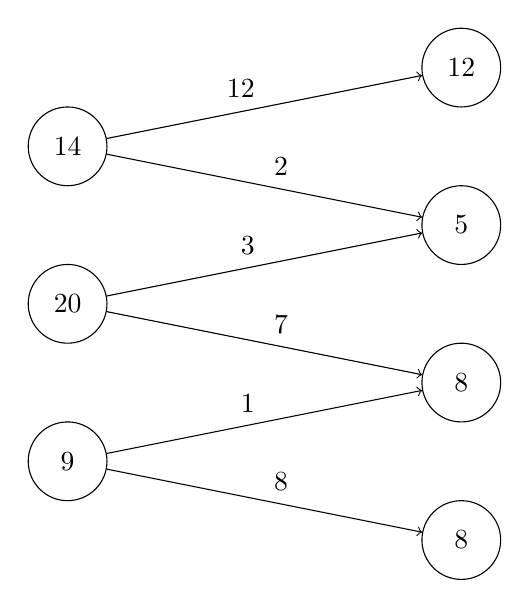
\begin{tikzpicture}[
            node distance=2cm,
            vertex/.style={
                circle,
                draw,
                minimum size=1cm,
                inner sep=0pt
            }
        ]

            \node[vertex] (s1) at (0, 2) {\(14\)};
            \node[vertex] (s2) at (0, 0) {\(20\)};
            \node[vertex] (s3) at (0, -2) {\(9\)};


            \node[vertex] (d1) at (5, 3) {\(12\)};
            \node[vertex] (d2) at (5, 1) {\(5\)};
            \node[vertex] (d3) at (5, -1) {\(8\)};
            \node[vertex] (d4) at (5, -3) {\(8\)};

            \draw[->] (s1) -- (d1)
                node[midway, above left] {\(12\)};
            \draw[->] (s1) -- (d2)
                node[midway, above right] {\(2\)};

            \draw[->] (s2) -- (d2)
                node[midway, above left] {\(3\)};
            \draw[->] (s2) -- (d3)
                node[midway, above right] {\(7\)};

            \draw[->] (s3) -- (d3)
                node[midway, above left] {\(1\)};
            \draw[->] (s3) -- (d4)
                node[midway, above right] {\(8\)};

        \end{tikzpicture}
    \end{center}
    with the flow matrix
    \[
        \pqty{x_{ij}} = \pmqty{
            12 & 2 & 0 & 0 \\
            0 & 3 & 7 & 0 \\
            0 & 0 & 1 & 8
        }.
    \]

    We now calculate the dual variables. By complementary slackness, we must have
    \begin{align*}
        \lambda_1 + \mu_1 = 5, & \quad \lambda_1 + \mu_2 = 3, \\
        \lambda_2 + \mu_2 = 7, & \quad \lambda_2 + \mu_3 = 4, \\
        \lambda_3 + \mu_3 = 2, & \quad \lambda_3 + \mu_4 = 4.
    \end{align*}

    Setting \(\lambda_1 = 0\), we solve to get
    \[
        \vb*{\lambda} = \pqty{0, 4, 2}\transpose \qand \vb*{\mu} = \pqty{5, 3, 0, 2}\transpose
    \]

    We can put this into a transport tableau:
    \[
        \renewcommand{\arraystretch}{1.5}
        \begin{array}{c
            !{\vrule width 1.2pt}
            cc|cc|cc|cc|c}

            \multicolumn{1}{c}{} &
            \multicolumn{2}{c}{5} &
            \multicolumn{2}{c}{3} &
            \multicolumn{2}{c}{0} &
            \multicolumn{2}{c}{2} &
            \\

            \noalign{\global\arrayrulewidth=1.2pt}
            \cline{2-9}
            \noalign{\global\arrayrulewidth=0.4pt}

            \multirow{2}{*}{\(0\)}
            &
            \multicolumn{2}{c|}{5} &
            \multicolumn{2}{c|}{3} &
            \multicolumn{2}{c|}{0} &
            \multicolumn{2}{c!{\vrule width 1.2pt}}{2} &
            \multirow{2}{*}{\(14\)}
            \\

            \cline{3-3}
            \cline{5-5}
            \cline{7-7}
            \cline{9-9}

            &
            12 & \multicolumn{1}{|c|}{5} &
            2  & \multicolumn{1}{|c|}{3} &
            0  & \multicolumn{1}{|c|}{4} &
            0  & \multicolumn{1}{|c!{\vrule width 1.2pt}}{6} &
            \\

            \cline{2-9}

            \multirow{2}{*}{\(4\)}
            &
            \multicolumn{2}{c|}{\boxed{9^{\ast}}} &
            \multicolumn{2}{c|}{7} &
            \multicolumn{2}{c|}{4} &
            \multicolumn{2}{c!{\vrule width 1.2pt}}{\boxed{6}} &
            \multirow{2}{*}{\(10\)}
            \\

            \cline{3-3}
            \cline{5-5}
            \cline{7-7}
            \cline{9-9}

            &
            0 & \multicolumn{1}{|c|}{2} &
            3 & \multicolumn{1}{|c|}{7} &
            7 & \multicolumn{1}{|c|}{4} &
            0 & \multicolumn{1}{|c!{\vrule width 1.2pt}}{1} &
            \\

            \cline{2-9}

            \multirow{2}{*}{\(2\)}
            &
            \multicolumn{2}{c|}{\boxed{7}} &
            \multicolumn{2}{c|}{5} &
            \multicolumn{2}{c|}{2} &
            \multicolumn{2}{c!{\vrule width 1.2pt}}{4} &
            \multirow{2}{*}{\(9\)}
            \\

            \cline{3-3}
            \cline{5-5}
            \cline{7-7}
            \cline{9-9}

            &
            0 & \multicolumn{1}{|c|}{5} &
            0 & \multicolumn{1}{|c|}{6} &
            1 & \multicolumn{1}{|c|}{2} &
            8 & \multicolumn{1}{|c!{\vrule width 1.2pt}}{4} &
            \\

            \noalign{\global\arrayrulewidth=1.2pt}
            \cline{2-9}
            \noalign{\global\arrayrulewidth=0.4pt}

            \multicolumn{1}{c}{} &
            \multicolumn{2}{c}{12} &
            \multicolumn{2}{c}{5} &
            \multicolumn{2}{c}{8} &
            \multicolumn{2}{c}{8} &

        \end{array}
        \renewcommand{\arraystretch}{1}
    \]

    Observe that the boxed entries do not satisfy the optimality conditions. Looking at the \(9, 0, 2\) entry, using ideas from the simplex algorithm, this means we need to add an edge from the second supplier to the first consumer, and push as much flow onto it as possible. Say the weight reassigned onto this new edge is \(\theta\).

    \begin{center}
        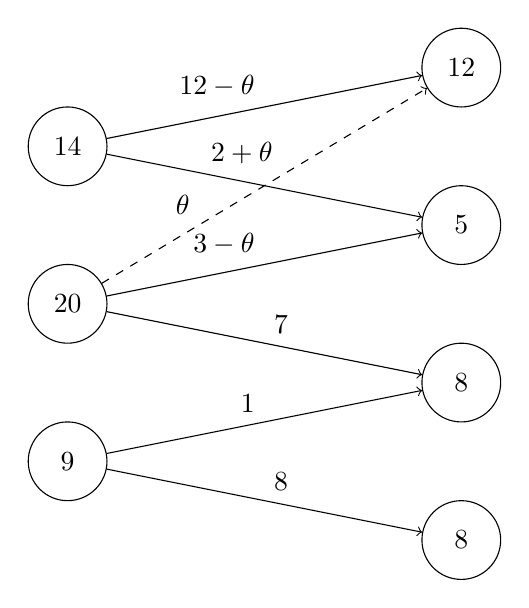
\begin{tikzpicture}[
            node distance=2cm,
            vertex/.style={
                circle,
                draw,
                minimum size=1cm,
                inner sep=0pt
            }
        ]

            \node[vertex] (s1) at (0, 2) {\(14\)};
            \node[vertex] (s2) at (0, 0) {\(20\)};
            \node[vertex] (s3) at (0, -2) {\(9\)};


            \node[vertex] (d1) at (5, 3) {\(12\)};
            \node[vertex] (d2) at (5, 1) {\(5\)};
            \node[vertex] (d3) at (5, -1) {\(8\)};
            \node[vertex] (d4) at (5, -3) {\(8\)};

            \draw[->] (s1) -- (d1)
                node[midway, above left] {\(12 - \theta\)};
            \draw[->] (s1) -- (d2)
                node[pos=0.3, above right] {\(2 + \theta\)};

            \draw[->, dashed] (s2) -- (d1)
                node[pos=0.3, above left] {\(\theta\)};

            \draw[->] (s2) -- (d2)
                node[midway, above left] {\(3 - \theta\)};
            \draw[->] (s2) -- (d3)
                node[midway, above right] {\(7\)};

            \draw[->] (s3) -- (d3)
                node[midway, above left] {\(1\)};
            \draw[->] (s3) -- (d4)
                node[midway, above right] {\(8\)};

        \end{tikzpicture}
    \end{center}

    Set \(\theta = 3\) since any \(\theta\) greater than this would mean a negative flow. This gives the new flow diagram
    \begin{center}
        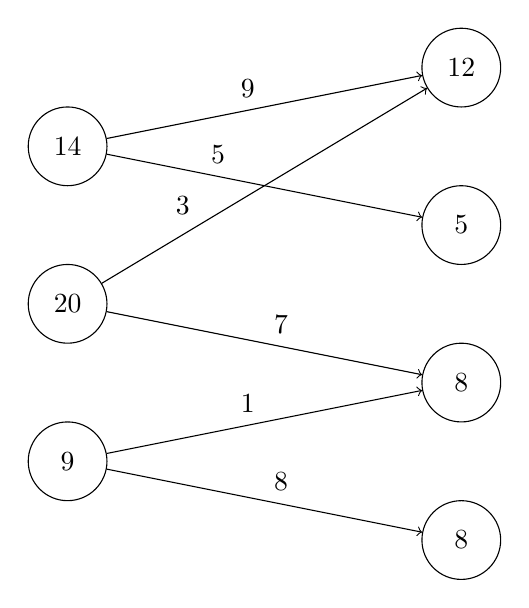
\begin{tikzpicture}[
            node distance=2cm,
            vertex/.style={
                circle,
                draw,
                minimum size=1cm,
                inner sep=0pt
            }
        ]

            \node[vertex] (s1) at (0, 2) {\(14\)};
            \node[vertex] (s2) at (0, 0) {\(20\)};
            \node[vertex] (s3) at (0, -2) {\(9\)};


            \node[vertex] (d1) at (5, 3) {\(12\)};
            \node[vertex] (d2) at (5, 1) {\(5\)};
            \node[vertex] (d3) at (5, -1) {\(8\)};
            \node[vertex] (d4) at (5, -3) {\(8\)};

            \draw[->] (s1) -- (d1)
                node[midway, above left] {\(9\)};
            \draw[->] (s1) -- (d2)
                node[pos=0.3, above right] {\(5\)};

            \draw[->] (s2) -- (d1)
                node[pos=0.3, above left] {\(3\)};
            \draw[->] (s2) -- (d3)
                node[midway, above right] {\(7\)};

            \draw[->] (s3) -- (d3)
                node[midway, above left] {\(1\)};
            \draw[->] (s3) -- (d4)
                node[midway, above right] {\(8\)};

        \end{tikzpicture}
    \end{center}
    with the transport tableau
    \[
        \renewcommand{\arraystretch}{1.5}
        \begin{array}{c
            !{\vrule width 1.2pt}
            cc|cc|cc|cc|c}

            \multicolumn{1}{c}{} &
            \multicolumn{2}{c}{5} &
            \multicolumn{2}{c}{3} &
            \multicolumn{2}{c}{7} &
            \multicolumn{2}{c}{9} &
            \\

            \noalign{\global\arrayrulewidth=1.2pt}
            \cline{2-9}
            \noalign{\global\arrayrulewidth=0.4pt}

            \multirow{2}{*}{\(0\)}
            &
            \multicolumn{2}{c|}{5} &
            \multicolumn{2}{c|}{3} &
            \multicolumn{2}{c|}{\boxed{7}} &
            \multicolumn{2}{c!{\vrule width 1.2pt}}{\boxed{9}} &
            \multirow{2}{*}{\(14\)}
            \\

            \cline{3-3}
            \cline{5-5}
            \cline{7-7}
            \cline{9-9}

            &
            9 & \multicolumn{1}{|c|}{5} &
            5  & \multicolumn{1}{|c|}{3} &
            0  & \multicolumn{1}{|c|}{4} &
            0  & \multicolumn{1}{|c!{\vrule width 1.2pt}}{6} &
            \\

            \cline{2-9}

            \multirow{2}{*}{\(-3\)}
            &
            \multicolumn{2}{c|}{2} &
            \multicolumn{2}{c|}{3} &
            \multicolumn{2}{c|}{4} &
            \multicolumn{2}{c!{\vrule width 1.2pt}}{\boxed{6^{\ast}}} &
            \multirow{2}{*}{\(10\)}
            \\

            \cline{3-3}
            \cline{5-5}
            \cline{7-7}
            \cline{9-9}

            &
            3 & \multicolumn{1}{|c|}{2} &
            0 & \multicolumn{1}{|c|}{7} &
            7 & \multicolumn{1}{|c|}{4} &
            0 & \multicolumn{1}{|c!{\vrule width 1.2pt}}{1} &
            \\

            \cline{2-9}

            \multirow{2}{*}{\(-5\)}
            &
            \multicolumn{2}{c|}{0} &
            \multicolumn{2}{c|}{-2} &
            \multicolumn{2}{c|}{2} &
            \multicolumn{2}{c!{\vrule width 1.2pt}}{4} &
            \multirow{2}{*}{\(9\)}
            \\

            \cline{3-3}
            \cline{5-5}
            \cline{7-7}
            \cline{9-9}

            &
            0 & \multicolumn{1}{|c|}{5} &
            0 & \multicolumn{1}{|c|}{6} &
            1 & \multicolumn{1}{|c|}{2} &
            8 & \multicolumn{1}{|c!{\vrule width 1.2pt}}{4} &
            \\

            \noalign{\global\arrayrulewidth=1.2pt}
            \cline{2-9}
            \noalign{\global\arrayrulewidth=0.4pt}

            \multicolumn{1}{c}{} &
            \multicolumn{2}{c}{12} &
            \multicolumn{2}{c}{5} &
            \multicolumn{2}{c}{8} &
            \multicolumn{2}{c}{8} &

        \end{array}
        \renewcommand{\arraystretch}{1}
    \]

    We now deal with the \(6, 0, 1\) entry. This adds the new edge
    \begin{center}
        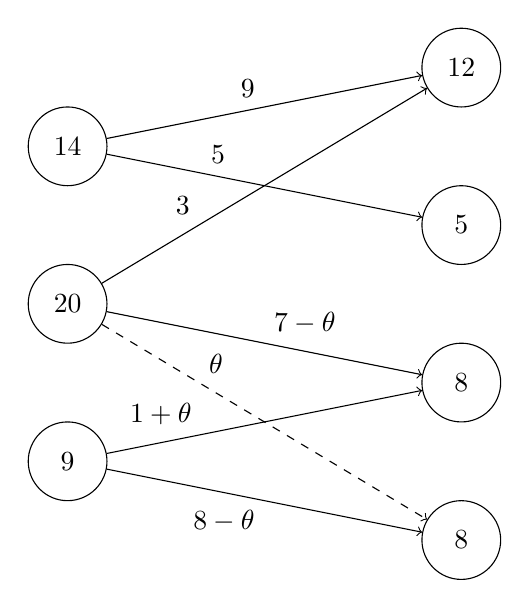
\begin{tikzpicture}[
            node distance=2cm,
            vertex/.style={
                circle,
                draw,
                minimum size=1cm,
                inner sep=0pt
            }
        ]

            \node[vertex] (s1) at (0, 2) {\(14\)};
            \node[vertex] (s2) at (0, 0) {\(20\)};
            \node[vertex] (s3) at (0, -2) {\(9\)};


            \node[vertex] (d1) at (5, 3) {\(12\)};
            \node[vertex] (d2) at (5, 1) {\(5\)};
            \node[vertex] (d3) at (5, -1) {\(8\)};
            \node[vertex] (d4) at (5, -3) {\(8\)};

            \draw[->] (s1) -- (d1)
                node[midway, above left] {\(9\)};
            \draw[->] (s1) -- (d2)
                node[pos=0.3, above right] {\(5\)};

            \draw[->] (s2) -- (d1)
                node[pos=0.3, above left] {\(3\)};
            \draw[->] (s2) -- (d3)
                node[midway, above right] {\(7 - \theta\)};

            \draw[->] (s3) -- (d3)
                node[pos=0.3, above left] {\(1 + \theta\)};
            \draw[->] (s3) -- (d4)
                node[midway, below left] {\(8 - \theta\)};

            \draw[->, dashed] (s2) -- (d4)
                node[pos=0.3, above right] {\(\theta\)};

        \end{tikzpicture}
    \end{center}
    and we maximise to get \(\theta = 7\), giving the new flow diagram
        \begin{center}
        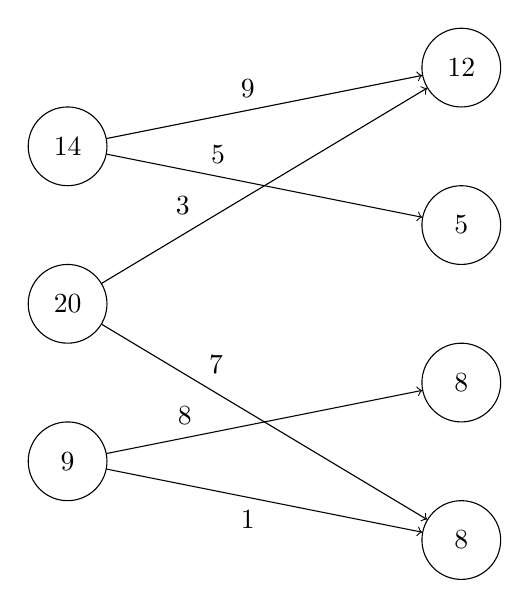
\begin{tikzpicture}[
            node distance=2cm,
            vertex/.style={
                circle,
                draw,
                minimum size=1cm,
                inner sep=0pt
            }
        ]

            \node[vertex] (s1) at (0, 2) {\(14\)};
            \node[vertex] (s2) at (0, 0) {\(20\)};
            \node[vertex] (s3) at (0, -2) {\(9\)};


            \node[vertex] (d1) at (5, 3) {\(12\)};
            \node[vertex] (d2) at (5, 1) {\(5\)};
            \node[vertex] (d3) at (5, -1) {\(8\)};
            \node[vertex] (d4) at (5, -3) {\(8\)};

            \draw[->] (s1) -- (d1)
                node[midway, above left] {\(9\)};
            \draw[->] (s1) -- (d2)
                node[pos=0.3, above right] {\(5\)};

            \draw[->] (s2) -- (d1)
                node[pos=0.3, above left] {\(3\)};

            \draw[->] (s3) -- (d3)
                node[pos=0.3, above left] {\(8\)};
            \draw[->] (s3) -- (d4)
                node[midway, below left] {\(1\)};

            \draw[->] (s2) -- (d4)
                node[pos=0.3, above right] {\(7\)};

        \end{tikzpicture}
    \end{center}
    and transport tableau
    \[
        \renewcommand{\arraystretch}{1.5}
        \begin{array}{c
            !{\vrule width 1.2pt}
            cc|cc|cc|cc|c}

            \multicolumn{1}{c}{} &
            \multicolumn{2}{c}{5} &
            \multicolumn{2}{c}{3} &
            \multicolumn{2}{c}{2} &
            \multicolumn{2}{c}{4} &
            \\

            \noalign{\global\arrayrulewidth=1.2pt}
            \cline{2-9}
            \noalign{\global\arrayrulewidth=0.4pt}

            \multirow{2}{*}{\(0\)}
            &
            \multicolumn{2}{c|}{5} &
            \multicolumn{2}{c|}{3} &
            \multicolumn{2}{c|}{2} &
            \multicolumn{2}{c!{\vrule width 1.2pt}}{4} &
            \multirow{2}{*}{\(14\)}
            \\

            \cline{3-3}
            \cline{5-5}
            \cline{7-7}
            \cline{9-9}

            &
            9 & \multicolumn{1}{|c|}{5} &
            5  & \multicolumn{1}{|c|}{3} &
            0  & \multicolumn{1}{|c|}{4} &
            0  & \multicolumn{1}{|c!{\vrule width 1.2pt}}{6} &
            \\

            \cline{2-9}

            \multirow{2}{*}{\(-3\)}
            &
            \multicolumn{2}{c|}{2} &
            \multicolumn{2}{c|}{0} &
            \multicolumn{2}{c|}{-1} &
            \multicolumn{2}{c!{\vrule width 1.2pt}}{1} &
            \multirow{2}{*}{\(10\)}
            \\

            \cline{3-3}
            \cline{5-5}
            \cline{7-7}
            \cline{9-9}

            &
            3 & \multicolumn{1}{|c|}{2} &
            0 & \multicolumn{1}{|c|}{7} &
            0 & \multicolumn{1}{|c|}{4} &
            7 & \multicolumn{1}{|c!{\vrule width 1.2pt}}{1} &
            \\

            \cline{2-9}

            \multirow{2}{*}{\(0\)}
            &
            \multicolumn{2}{c|}{5} &
            \multicolumn{2}{c|}{3} &
            \multicolumn{2}{c|}{2} &
            \multicolumn{2}{c!{\vrule width 1.2pt}}{4} &
            \multirow{2}{*}{\(9\)}
            \\

            \cline{3-3}
            \cline{5-5}
            \cline{7-7}
            \cline{9-9}

            &
            0 & \multicolumn{1}{|c|}{5} &
            0 & \multicolumn{1}{|c|}{6} &
            8 & \multicolumn{1}{|c|}{2} &
            1 & \multicolumn{1}{|c!{\vrule width 1.2pt}}{4} &
            \\

            \noalign{\global\arrayrulewidth=1.2pt}
            \cline{2-9}
            \noalign{\global\arrayrulewidth=0.4pt}

            \multicolumn{1}{c}{} &
            \multicolumn{2}{c}{12} &
            \multicolumn{2}{c}{5} &
            \multicolumn{2}{c}{8} &
            \multicolumn{2}{c}{8} &

        \end{array}
        \renewcommand{\arraystretch}{1}
    \]

    This satisfies the optimality conditions, hence solves the problem.
\end{example}

\subsection{Maximum Flow and Minimum Cut}
\subsubsection{Maximum Flow}

We now consider a directed graph with \term{capacities} assigned to each edges. We want to maximise the flow from the source to the sink by assigning flows along each edge, while not exceeding the capacities of each edge. (Of course, the flow conservation equation must be satisfied). Without loss of generality, assume the source vertex is \(1\) and the sink vertex is \(n\).

\begin{definition}[Maximum Flow Problem]
    For a graph \(G = \pqty{V, E}\) and a matrix \(c_{ij}\) defined on its edges (the capacities of each edge), the \term{maximum flow problem} is to \emph{maximise} \(\delta\), the flow, subject to constraints
    \begin{itemize}
        \item \term{outgoing flow} from vertex \(1\):
        \[
            \sum_{j: \pqty{1, j} \in E} x_{1j} - \sum_{i: \pqty{i, 1} \in E} x_{i1} = \delta;
        \]
        \item \term{incoming flow} to vertex \(n\):
        \[
            \sum_{i: \pqty{i, n} \in E} x_{in} - \sum_{j: \pqty{n, j} \in E} x_{nj} = \delta;
        \]
        \item \term{flow conservation} at vertex \(i \neq 1, n\):
        \[
            \sum_{j: \pqty{i, j} \in E} x_{ij} = \sum_{j: \pqty{j, i} \in E} x_{ji};
        \]
        \item \term{capacity constraint}: for all \(\pqty{i, j} \in E\),
        \[
            0 \leq x_{ij} \leq c_{ij}.
        \]
    \end{itemize}
\end{definition}

\begin{notation}
    Introducing the notation for the net amount of flow leaving a node
    \[
        \phi_i \pqty{x} = \sum_{j: \pqty{i, j} \in E} x_{ij} - \sum_{j: \pqty{j, i} \in E} x_{ji}
    \]
    and an indicator
    \[
        b_i = \begin{cases}
            +1, &\qif i = 1, \\
            -1, &\qif i = n, \\
            0, &\qotherwise.
        \end{cases}
    \]
    then the problem became maximising \(\delta\), subject to constraints
    \[
        \phi_i \pqty{x} - b_i \delta = 0
    \]
    for all \(i\), and \(0 \leq x_{ij} \leq c_{ij}\).
\end{notation}

\subsubsection{Minimum Cut and Augmenting Paths}

Another problem is related to \term{cuts} of a graph.

\begin{definition}[Cut of a Graph, Capacity of a Cut]
    A \term{cut} of a graph \(G = \pqty{V, E}\) is a partition of \(V\) into two sets, \(\pqty{S, V \setminus S}\).
    
    The \term{capacity} of the cut is the sum of the capacities crossing the cut
    \[
        C\pqty{S} = \sum_{\substack{i \in S \\ j \in V \setminus S \\ \pqty{i, j} \in E}} c_{ij}.
    \]
\end{definition}

\begin{theorem}[Maximum Flow is Upper Bounded by \(C\pqty{S}\)]
    Let \(\pqty{x_{ij}}\) be a feasible flow with flow value \(\delta\). For any cut \(\pqty{S, V \setminus S}\) such that \(1 \in S\) and \(n \in V \setminus S\), we have
    \[
        \delta \leq C\pqty{S}.
    \]
\end{theorem}

\begin{remark}
    This states that
    \[
        \max_{\pqty{x_{ij}}} \delta \leq \min_{\substack{S \subseteq V \\ 1 \in S,\ n \notin S}} C\pqty{S}.
    \]
\end{remark}

\begin{proof}
    For \(A, B \subseteq V\) (not necessarily disjoint), we define
    \[
        f_x \pqty{A, B} = \sum_{\substack{i \in A \\ j \in B \\ \pqty{i, j} \in E}} x_{ij}.
    \]

    Note that
    \[
        C\pqty{S} \geq f_x \pqty{S, V \setminus S}
    \]
    since \(c_{ij} \geq x_{ij}\).

    We sum up the flow constraint for all \(i \in S\), which gives
    \begin{align*}
        \sum_{i \in S} \phi_i \pqty{x} &= \sum_{i \in S} \pqty{\sum_{j: \pqty{i, j} \in E} x_{ij} - \sum_{j: \pqty{i, j} \in E} x_{ji}} \\
        &= \sum_{i \in S} b_i \delta \\
        &= \delta
    \end{align*}
    and hence
    \begin{align*}
        \delta &= f_x \pqty{S, V} - f_x \pqty{V, S} \\
        &= f_x \pqty{S, S} + f_x \pqty{S, V \setminus S} - f_x \pqty{S, S} - f_x \pqty{V \setminus S, S} \\
        &= f_x \pqty{S, V \setminus S} - f_x \pqty{V \setminus S, S} \\
        &\leq f_x \pqty{S, V \setminus S} \\
        &\leq C \pqty{S}.
    \end{align*}
\end{proof}

To help our proof that minimum cut is in fact equal to maximum flow, we introduce the following definition.

\begin{definition}[Path, Augmenting Path]
    A \term{undirected path} is a sequence of distinct vertices \(v_0, v_1, \ldots, v_k\), satisfying \(\pqty{v_{i - 1}, v_i} \in E\) or \(\pqty{v_i, v_{i - 1}} \in E\) for all \(i = 1, 2, \ldots, k\).

    An \term{augmenting path} is a path such that, for every \(i = 1, 2, \ldots, k\), at least one of the following holds:
    \begin{itemize}
        \item \term{forward edge with non-optimal flow}: \(\pqty{v_{i - 1}, v_i} \in E\) and \(x_{v_{i - 1} v_i} < c_{v_{i - 1} v_i}\);
        \item \term{reverse edge with positive flow}: \(\pqty{v_i, v_{i - 1}} \in E\) and \(x_{v_i v_{i - 1}} > 0\).
    \end{itemize}
\end{definition}

\begin{lemma}[Non-Existence of Augmenting Paths between \(1\) and \(n\) in Optimal Flow]
    If a flow \(\pqty{x_{ij}}\) is optimal, then it does not contain an augmenting path between \(1\) and \(n\).
\end{lemma}

\begin{proof}
    If an augmenting path exists, we could increase the flow along that path by increasing the flow on forward edges by \(\epsilon\) and decreasing the flow on backward edges by \(\epsilon\), for sufficiently small \(\epsilon > 0\), without violating constraints.
\end{proof}

\begin{theorem}[Maximum Flow is Minimum Cut]
    \label{thm:max-flow-min-cut}%
    Let \(\delta^{\ast}\) be the maximum value of the flow. Then
    \[
        \delta^{\ast} = \min \set{C \pqty{S}}{S \subseteq V, 1 \in S, n \in V \setminus S}.
    \]
\end{theorem}

\begin{proof}
    It suffices to produce a set \(S\) such that \(C\pqty{S} = \delta^{\ast}\).

    If a flow \(x\) is optimal, then \(x\) cannot have augmenting paths from \(1\) to \(n\). Define
    \[
        S = \set{1} \cup \set{i \in V}{\text{there exists augmenting path from }1\text{ to }i}
    \]
    and observe \(1 \in S\) while \(n \notin S\). For this set \(S\), sum up the flow constraints of \(S\),
    \[
        \delta^{\ast} = f_x \pqty{S, V \setminus S} - f_x \pqty{V \setminus S, S}.
    \]

    Notice that any \(i \in S\), \(j \in V \setminus S\) and \(\pqty{i, j} \in E\) must satisfy that \(x_{ij} = c_{ij}\) (otherwise we could extend an augmenting path to \(j\)); and similarly for any \(i \in S\), \(j \in V \setminus S\) and \(\pqty{j, i} \in E\) must satisfy that \(x_{ij} = 0\). Hence,
    \[
        f_x \pqty{S, V \setminus S} = C\pqty{S} \qand f_x \pqty{V \setminus S, S} = 0
    \]
    hence
    \[
        \delta^{\ast} = C\pqty{S}.
    \]
\end{proof}

\subsubsection{The Ford--Fulkerson Algorithm}

The Ford--Fulkerson Algorithm arising from \autoref{thm:max-flow-min-cut} augments the augmenting paths from \(1\) to \(n\), and is described as follows.

\begin{itemize}
    \item Start from a feasible flow \(\pqty{x_{ij}}\), say the trivial flow with all zeros.
    \item While we can find an augmenting path between \(1\) and \(n\), optimise the flow (by increasing the forward flow) until it is not an augmenting path.
    \item When there are no augmenting paths, 
\end{itemize}

It could be tedious to list all possible paths, so if at one point one fails to find an augmenting path between \(1\) and \(n\), it could be useful to stop and attempt to construct a cut with the same capacity as the flow, at which point we could stop.

\begin{example}[Ford--Fulkerson Algorithm, First Example]
    Consider the following network. (At the moment all flow is zero, and the capacities are boxed.)

    \begin{center}
        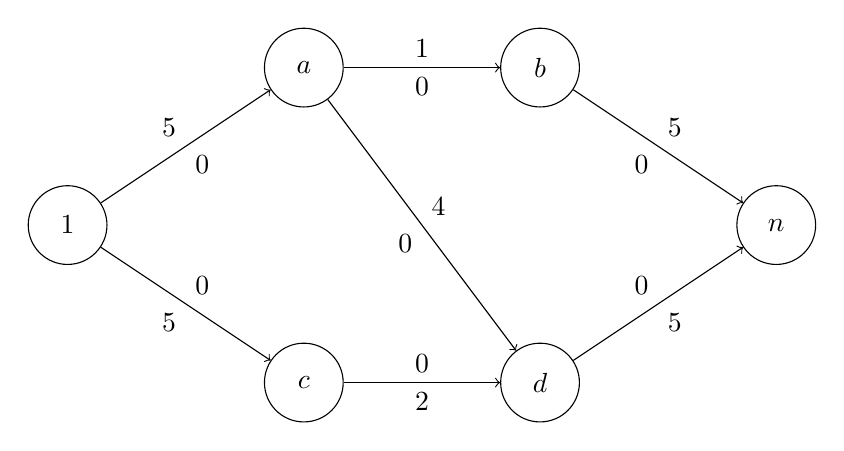
\begin{tikzpicture}[
            node distance=2cm,
            vertex/.style={
                circle,
                draw,
                minimum size=1cm,
                inner sep=0pt
            }
        ]

            \node[vertex] (1) at (0, 0) {\(1\)};
            \node[vertex] (a) at (3, 2) {\(a\)};
            \node[vertex] (c) at (3, -2) {\(c\)};
            \node[vertex] (b) at (6, 2) {\(b\)};
            \node[vertex] (d) at (6, -2) {\(d\)};
            \node[vertex] (n) at (9, 0) {\(n\)};

            \draw[->] (1) -- (a)
                node[midway, above left] {\(\boxed{5}\)}
                node[midway, below right] {\(0\)};

            \draw[->] (a) -- (b)
                node[midway, above] {\(\boxed{1}\)}
                node[midway, below] {\(0\)};

            \draw[->] (b) -- (n)
                node[midway, above right] {\(\boxed{5}\)}
                node[midway, below left] {\(0\)};

            \draw[->] (1) -- (c)
                node[midway, below left] {\(\boxed{5}\)}
                node[midway, above right] {\(0\)};

            \draw[->] (c) -- (d)
                node[midway, below] {\(\boxed{2}\)}
                node[midway, above] {\(0\)};

            \draw[->] (d) -- (n)
                node[midway, below right] {\(\boxed{5}\)}
                node[midway, above left] {\(0\)};

            \draw[->] (a) -- (d)
                node[midway, above right] {\(\boxed{4}\)}
                node[midway, below left] {\(0\)};
        \end{tikzpicture}
    \end{center}

    All the paths from \(1\) to \(n\) are:
    \begin{itemize}
        \item \(1 \to a \to b \to n\);
        \item \(1 \to a \to d \to n\);
        \item \(1 \to c \to d \to n\).
    \end{itemize}

    Augmenting the path \(1 \to a \to b \to n\), we increase the flow along this by \(1\), giving the value of the flow as \(1\):
    \begin{center}
        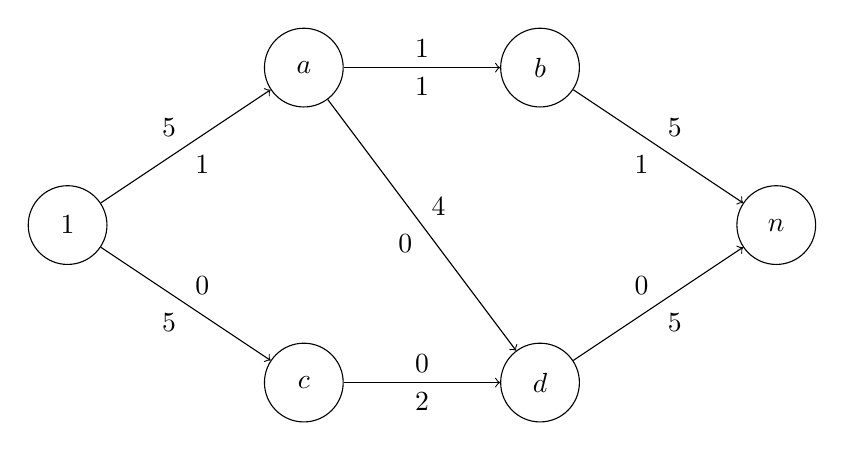
\begin{tikzpicture}[
            node distance=2cm,
            vertex/.style={
                circle,
                draw,
                minimum size=1cm,
                inner sep=0pt
            }
        ]

            \node[vertex] (1) at (0, 0) {\(1\)};
            \node[vertex] (a) at (3, 2) {\(a\)};
            \node[vertex] (c) at (3, -2) {\(c\)};
            \node[vertex] (b) at (6, 2) {\(b\)};
            \node[vertex] (d) at (6, -2) {\(d\)};
            \node[vertex] (n) at (9, 0) {\(n\)};

            \draw[->] (1) -- (a)
                node[midway, above left] {\(\boxed{5}\)}
                node[midway, below right] {\(1\)};

            \draw[->] (a) -- (b)
                node[midway, above] {\(\boxed{1}\)}
                node[midway, below] {\(1\)};

            \draw[->] (b) -- (n)
                node[midway, above right] {\(\boxed{5}\)}
                node[midway, below left] {\(1\)};

            \draw[->] (1) -- (c)
                node[midway, below left] {\(\boxed{5}\)}
                node[midway, above right] {\(0\)};

            \draw[->] (c) -- (d)
                node[midway, below] {\(\boxed{2}\)}
                node[midway, above] {\(0\)};

            \draw[->] (d) -- (n)
                node[midway, below right] {\(\boxed{5}\)}
                node[midway, above left] {\(0\)};

            \draw[->] (a) -- (d)
                node[midway, above right] {\(\boxed{4}\)}
                node[midway, below left] {\(0\)};
        \end{tikzpicture}
    \end{center}

    Augmenting the path \(1 \to a \to d \to n\), we increase the flow along this by \(4\), giving the value of the flow as \(5\):
    \begin{center}
        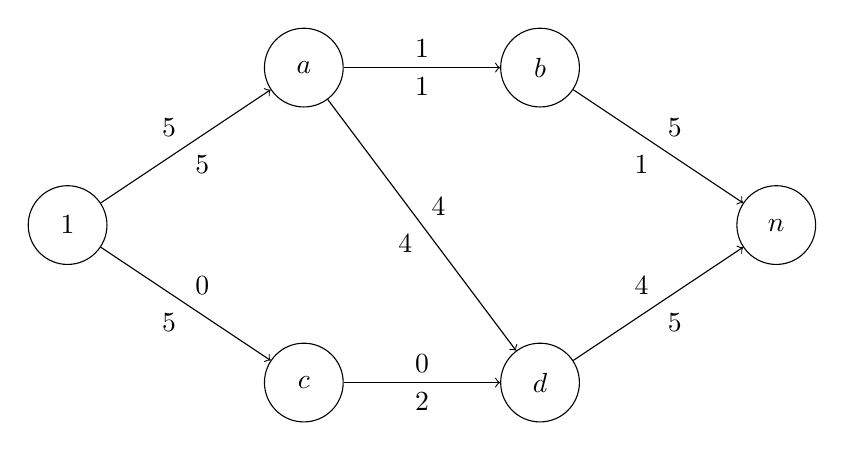
\begin{tikzpicture}[
            node distance=2cm,
            vertex/.style={
                circle,
                draw,
                minimum size=1cm,
                inner sep=0pt
            }
        ]

            \node[vertex] (1) at (0, 0) {\(1\)};
            \node[vertex] (a) at (3, 2) {\(a\)};
            \node[vertex] (c) at (3, -2) {\(c\)};
            \node[vertex] (b) at (6, 2) {\(b\)};
            \node[vertex] (d) at (6, -2) {\(d\)};
            \node[vertex] (n) at (9, 0) {\(n\)};

            \draw[->] (1) -- (a)
                node[midway, above left] {\(\boxed{5}\)}
                node[midway, below right] {\(5\)};

            \draw[->] (a) -- (b)
                node[midway, above] {\(\boxed{1}\)}
                node[midway, below] {\(1\)};

            \draw[->] (b) -- (n)
                node[midway, above right] {\(\boxed{5}\)}
                node[midway, below left] {\(1\)};

            \draw[->] (1) -- (c)
                node[midway, below left] {\(\boxed{5}\)}
                node[midway, above right] {\(0\)};

            \draw[->] (c) -- (d)
                node[midway, below] {\(\boxed{2}\)}
                node[midway, above] {\(0\)};

            \draw[->] (d) -- (n)
                node[midway, below right] {\(\boxed{5}\)}
                node[midway, above left] {\(4\)};

            \draw[->] (a) -- (d)
                node[midway, above right] {\(\boxed{4}\)}
                node[midway, below left] {\(4\)};
        \end{tikzpicture}
    \end{center}

    Augmenting the path \(1 \to b \to d \to n\), we increase the flow along this by \(1\), giving the value of the flow as \(6\):
    \begin{center}
        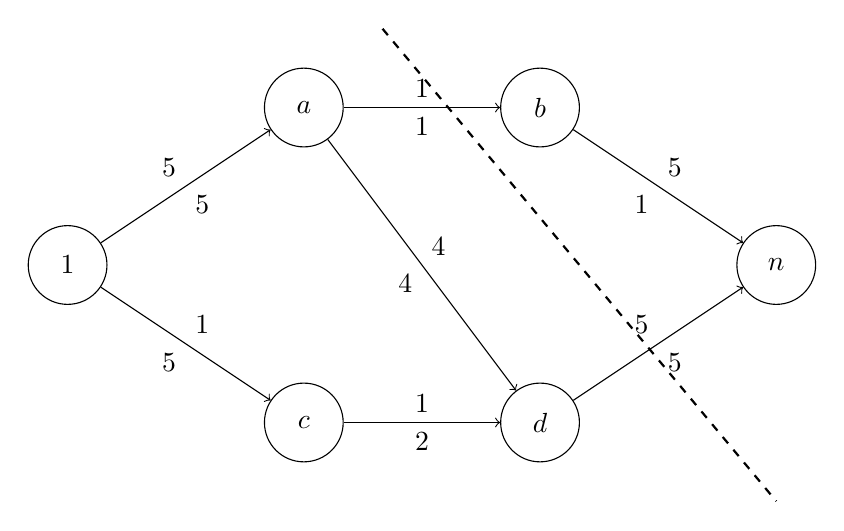
\begin{tikzpicture}[
            node distance=2cm,
            vertex/.style={
                circle,
                draw,
                minimum size=1cm,
                inner sep=0pt
            }
        ]

            \node[vertex] (1) at (0, 0) {\(1\)};
            \node[vertex] (a) at (3, 2) {\(a\)};
            \node[vertex] (c) at (3, -2) {\(c\)};
            \node[vertex] (b) at (6, 2) {\(b\)};
            \node[vertex] (d) at (6, -2) {\(d\)};
            \node[vertex] (n) at (9, 0) {\(n\)};

            \draw[->] (1) -- (a)
                node[midway, above left] {\(\boxed{5}\)}
                node[midway, below right] {\(5\)};

            \draw[->] (a) -- (b)
                node[midway, above] {\(\boxed{1}\)}
                node[midway, below] {\(1\)};

            \draw[->] (b) -- (n)
                node[midway, above right] {\(\boxed{5}\)}
                node[midway, below left] {\(1\)};

            \draw[->] (1) -- (c)
                node[midway, below left] {\(\boxed{5}\)}
                node[midway, above right] {\(1\)};

            \draw[->] (c) -- (d)
                node[midway, below] {\(\boxed{2}\)}
                node[midway, above] {\(1\)};

            \draw[->] (d) -- (n)
                node[midway, below right] {\(\boxed{5}\)}
                node[midway, above left] {\(5\)};

            \draw[->] (a) -- (d)
                node[midway, above right] {\(\boxed{4}\)}
                node[midway, below left] {\(4\)};

            \draw[dashed, thick] (4, 3) -- (9, -3);
        \end{tikzpicture}
    \end{center}

    Indeed, at this point, notice the cut \(S = \set{1, a, c, d}\) satisfies \(C\pqty{S} = 6\). This is hence the maximum flow (and the corresponding minimum cut).
\end{example}

\subsubsection{The Edmonds--Karp Algorithm and Convergence of the Ford--Fulkerson Algorithm}

One unsatisfying thing about the Ford--Fulkerson algorithm is it is not very obvious how this is related to the simplex algorithm. Indeed, the Ford--Fulkerson algorithm works relatively differently, in the sense that it does not necessarily jump to extreme points -- and hence convergence is not necessarily guaranteed (thought it is guaranteed to improve). In the case where all capacities are integral (in which case all increases are also integral) or rational (in which we could just scale the problem to be integral), it is guaranteed to converge after finitely many steps.

The Edmonds--Karp algorithm, which augments by increasing path length (i.e., finds such paths by breadth-first search), guarantees convergence in \(\bigO\pqty{\abs{V} \abs{E}^2}\) time.

\begin{example}[Ford--Fulkerson Algorithm, Second Example]
    Consider the following network. (At the moment all flow is zero, and the capacities are boxed.)

    \begin{center}
        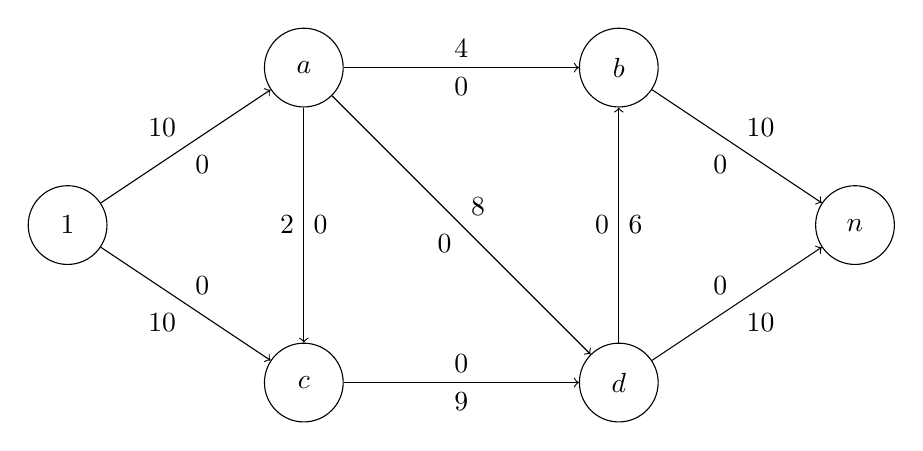
\begin{tikzpicture}[
            node distance=2cm,
            vertex/.style={
                circle,
                draw,
                minimum size=1cm,
                inner sep=0pt
            }
        ]

            \node[vertex] (1) at (0, 0) {\(1\)};
            \node[vertex] (a) at (3, 2) {\(a\)};
            \node[vertex] (c) at (3, -2) {\(c\)};
            \node[vertex] (b) at (7, 2) {\(b\)};
            \node[vertex] (d) at (7, -2) {\(d\)};
            \node[vertex] (n) at (10, 0) {\(n\)};



            \draw[->] (1) -- (a)
                node[midway, above left] {\(\boxed{10}\)}
                node[midway, below right] {\(0\)};

            \draw[->] (a) -- (b)
                node[midway, above] {\(\boxed{4}\)}
                node[midway, below] {\(0\)};

            \draw[->] (b) -- (n)
                node[midway, above right] {\(\boxed{10}\)}
                node[midway, below left] {\(0\)};

            \draw[->] (1) -- (c)
                node[midway, below left] {\(\boxed{10}\)}
                node[midway, above right] {\(0\)};

            \draw[->] (c) -- (d)
                node[midway, below] {\(\boxed{9}\)}
                node[midway, above] {\(0\)};

            \draw[->] (d) -- (n)
                node[midway, below right] {\(\boxed{10}\)}
                node[midway, above left] {\(0\)};

            \draw[->] (a) -- (c)
                node[midway, left] {\(\boxed{2}\)}
                node[midway, right] {\(0\)};

            \draw[->] (d) -- (b)
                node[midway, right] {\(\boxed{6}\)}
                node[midway, left] {\(0\)};

            \draw[->] (a) -- (d)
                node[midway, above right] {\(\boxed{8}\)}
                node[midway, below left] {\(0\)};
        \end{tikzpicture}
    \end{center}

    We find the augmenting paths. The first one would be \(1 \to a \to b \to n\), which has capacity \(4\) (increasing the value to 4), giving
    \begin{center}
        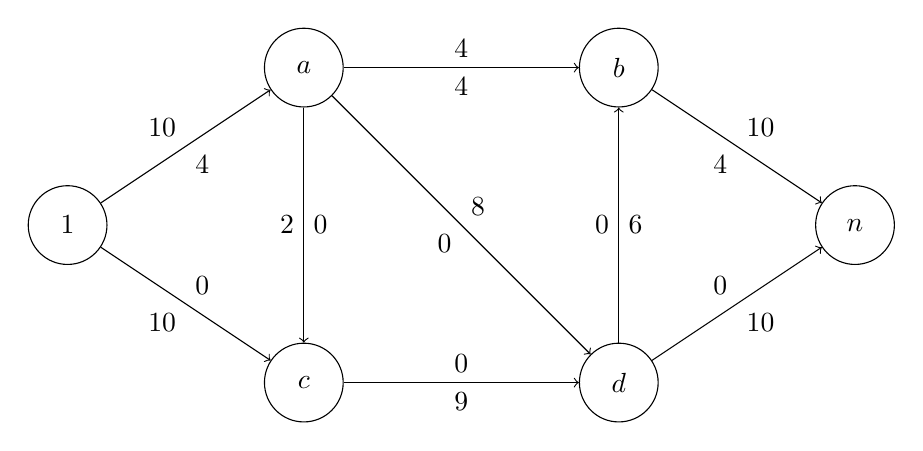
\begin{tikzpicture}[
            node distance=2cm,
            vertex/.style={
                circle,
                draw,
                minimum size=1cm,
                inner sep=0pt
            }
        ]

            \node[vertex] (1) at (0, 0) {\(1\)};
            \node[vertex] (a) at (3, 2) {\(a\)};
            \node[vertex] (c) at (3, -2) {\(c\)};
            \node[vertex] (b) at (7, 2) {\(b\)};
            \node[vertex] (d) at (7, -2) {\(d\)};
            \node[vertex] (n) at (10, 0) {\(n\)};



            \draw[->] (1) -- (a)
                node[midway, above left] {\(\boxed{10}\)}
                node[midway, below right] {\(4\)};

            \draw[->] (a) -- (b)
                node[midway, above] {\(\boxed{4}\)}
                node[midway, below] {\(4\)};

            \draw[->] (b) -- (n)
                node[midway, above right] {\(\boxed{10}\)}
                node[midway, below left] {\(4\)};

            \draw[->] (1) -- (c)
                node[midway, below left] {\(\boxed{10}\)}
                node[midway, above right] {\(0\)};

            \draw[->] (c) -- (d)
                node[midway, below] {\(\boxed{9}\)}
                node[midway, above] {\(0\)};

            \draw[->] (d) -- (n)
                node[midway, below right] {\(\boxed{10}\)}
                node[midway, above left] {\(0\)};

            \draw[->] (a) -- (c)
                node[midway, left] {\(\boxed{2}\)}
                node[midway, right] {\(0\)};

            \draw[->] (d) -- (b)
                node[midway, right] {\(\boxed{6}\)}
                node[midway, left] {\(0\)};

            \draw[->] (a) -- (d)
                node[midway, above right] {\(\boxed{8}\)}
                node[midway, below left] {\(0\)};
        \end{tikzpicture}
    \end{center}

    We look at \(1 \to a \to d \to n\), which has a capacity of \(6\) (increasing the value to 10), giving
    \begin{center}
        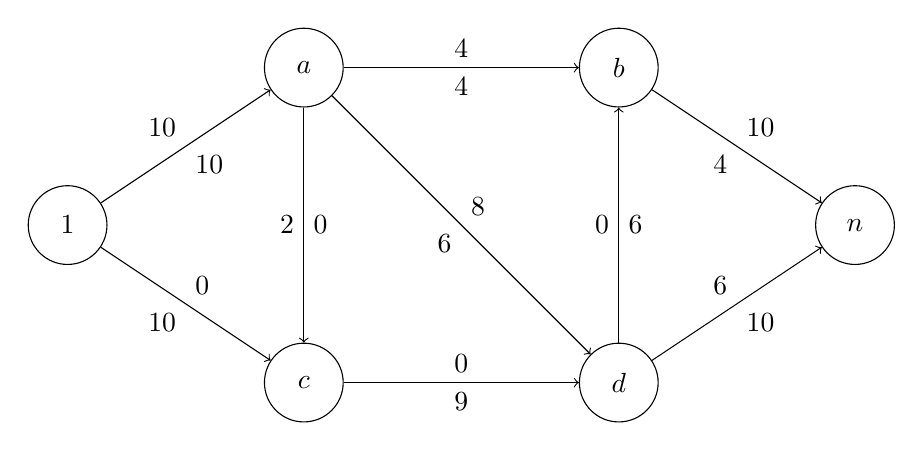
\begin{tikzpicture}[
            node distance=2cm,
            vertex/.style={
                circle,
                draw,
                minimum size=1cm,
                inner sep=0pt
            }
        ]

            \node[vertex] (1) at (0, 0) {\(1\)};
            \node[vertex] (a) at (3, 2) {\(a\)};
            \node[vertex] (c) at (3, -2) {\(c\)};
            \node[vertex] (b) at (7, 2) {\(b\)};
            \node[vertex] (d) at (7, -2) {\(d\)};
            \node[vertex] (n) at (10, 0) {\(n\)};



            \draw[->] (1) -- (a)
                node[midway, above left] {\(\boxed{10}\)}
                node[midway, below right] {\(10\)};

            \draw[->] (a) -- (b)
                node[midway, above] {\(\boxed{4}\)}
                node[midway, below] {\(4\)};

            \draw[->] (b) -- (n)
                node[midway, above right] {\(\boxed{10}\)}
                node[midway, below left] {\(4\)};

            \draw[->] (1) -- (c)
                node[midway, below left] {\(\boxed{10}\)}
                node[midway, above right] {\(0\)};

            \draw[->] (c) -- (d)
                node[midway, below] {\(\boxed{9}\)}
                node[midway, above] {\(0\)};

            \draw[->] (d) -- (n)
                node[midway, below right] {\(\boxed{10}\)}
                node[midway, above left] {\(6\)};

            \draw[->] (a) -- (c)
                node[midway, left] {\(\boxed{2}\)}
                node[midway, right] {\(0\)};

            \draw[->] (d) -- (b)
                node[midway, right] {\(\boxed{6}\)}
                node[midway, left] {\(0\)};

            \draw[->] (a) -- (d)
                node[midway, above right] {\(\boxed{8}\)}
                node[midway, below left] {\(6\)};
        \end{tikzpicture}
    \end{center}

    The next one would be \(1 \to c \to d \to n\), with a capacity of \(4\) (increasing the value to 14), giving
    \begin{center}
        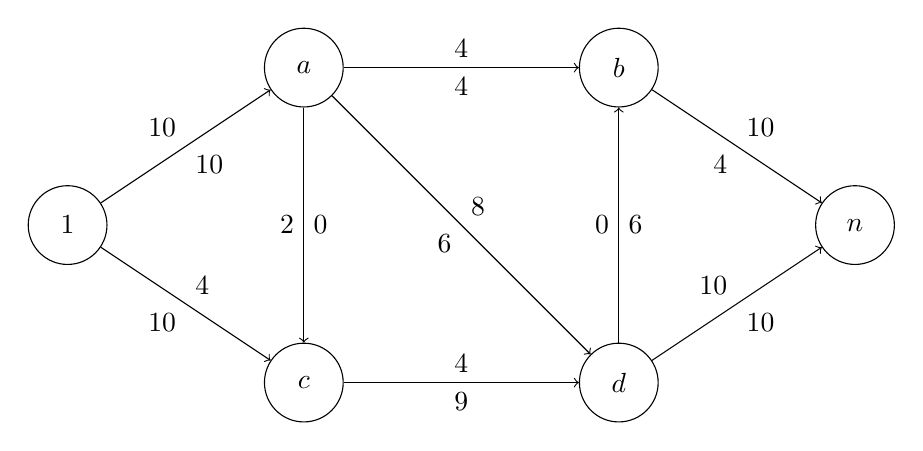
\begin{tikzpicture}[
            node distance=2cm,
            vertex/.style={
                circle,
                draw,
                minimum size=1cm,
                inner sep=0pt
            }
        ]

            \node[vertex] (1) at (0, 0) {\(1\)};
            \node[vertex] (a) at (3, 2) {\(a\)};
            \node[vertex] (c) at (3, -2) {\(c\)};
            \node[vertex] (b) at (7, 2) {\(b\)};
            \node[vertex] (d) at (7, -2) {\(d\)};
            \node[vertex] (n) at (10, 0) {\(n\)};



            \draw[->] (1) -- (a)
                node[midway, above left] {\(\boxed{10}\)}
                node[midway, below right] {\(10\)};

            \draw[->] (a) -- (b)
                node[midway, above] {\(\boxed{4}\)}
                node[midway, below] {\(4\)};

            \draw[->] (b) -- (n)
                node[midway, above right] {\(\boxed{10}\)}
                node[midway, below left] {\(4\)};

            \draw[->] (1) -- (c)
                node[midway, below left] {\(\boxed{10}\)}
                node[midway, above right] {\(4\)};

            \draw[->] (c) -- (d)
                node[midway, below] {\(\boxed{9}\)}
                node[midway, above] {\(4\)};

            \draw[->] (d) -- (n)
                node[midway, below right] {\(\boxed{10}\)}
                node[midway, above left] {\(10\)};

            \draw[->] (a) -- (c)
                node[midway, left] {\(\boxed{2}\)}
                node[midway, right] {\(0\)};

            \draw[->] (d) -- (b)
                node[midway, right] {\(\boxed{6}\)}
                node[midway, left] {\(0\)};

            \draw[->] (a) -- (d)
                node[midway, above right] {\(\boxed{8}\)}
                node[midway, below left] {\(6\)};
        \end{tikzpicture}
    \end{center}

    All paths of length 3 have been augmented, and therefore we look at paths of length 4. Augmenting the path \(1 \to c \to d \to b \to n\) increases the flow by \(5\) (increasing the value to \(19\)), which gives
    \begin{center}
        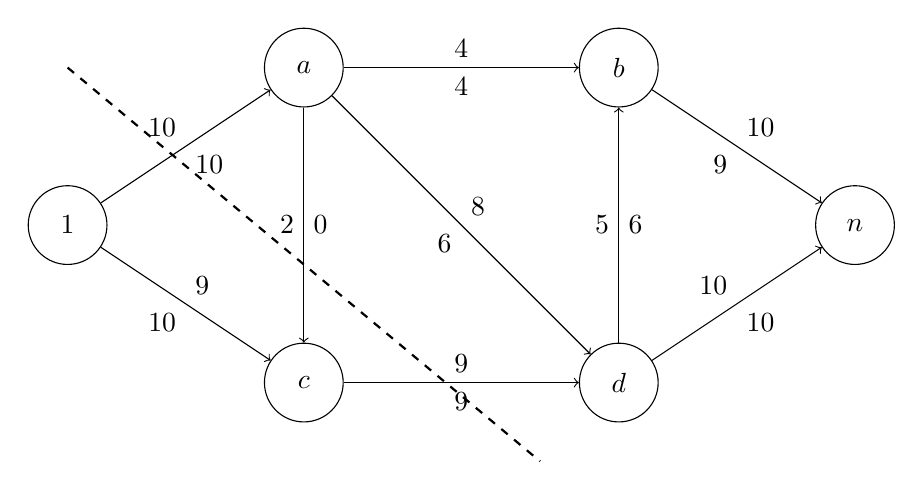
\begin{tikzpicture}[
            node distance=2cm,
            vertex/.style={
                circle,
                draw,
                minimum size=1cm,
                inner sep=0pt
            }
        ]

            \node[vertex] (1) at (0, 0) {\(1\)};
            \node[vertex] (a) at (3, 2) {\(a\)};
            \node[vertex] (c) at (3, -2) {\(c\)};
            \node[vertex] (b) at (7, 2) {\(b\)};
            \node[vertex] (d) at (7, -2) {\(d\)};
            \node[vertex] (n) at (10, 0) {\(n\)};



            \draw[->] (1) -- (a)
                node[midway, above left] {\(\boxed{10}\)}
                node[midway, below right] {\(10\)};

            \draw[->] (a) -- (b)
                node[midway, above] {\(\boxed{4}\)}
                node[midway, below] {\(4\)};

            \draw[->] (b) -- (n)
                node[midway, above right] {\(\boxed{10}\)}
                node[midway, below left] {\(9\)};

            \draw[->] (1) -- (c)
                node[midway, below left] {\(\boxed{10}\)}
                node[midway, above right] {\(9\)};

            \draw[->] (c) -- (d)
                node[midway, below] {\(\boxed{9}\)}
                node[midway, above] {\(9\)};

            \draw[->] (d) -- (n)
                node[midway, below right] {\(\boxed{10}\)}
                node[midway, above left] {\(10\)};

            \draw[->] (a) -- (c)
                node[midway, left] {\(\boxed{2}\)}
                node[midway, right] {\(0\)};

            \draw[->] (d) -- (b)
                node[midway, right] {\(\boxed{6}\)}
                node[midway, left] {\(5\)};

            \draw[->] (a) -- (d)
                node[midway, above right] {\(\boxed{8}\)}
                node[midway, below left] {\(6\)};

            \draw[dashed, thick] (0, 2) -- (6, -3);
        \end{tikzpicture}
    \end{center}

    Indeed, notice the cut \(S = \set{1, c}\) gives a cut of \(19\), and hence this must be optimal.
\end{example}

\subsubsection{Duality of Maximum Flow and Minimum Cut}

We have discussed a lot about duality of problems in this course, and it is very tempting to prove that maximum flow corresponding to minimum cut is a duality problem. (This is also suggested by our two-part theorem proof.) However, it is not immediately clear how minimum cut can be a linear programming problem.

Recall the notation
\[
    b_i = \begin{cases}
        +1, &\qif i = 1, \\
        -1, &\qif i = n, \\
        0, &\qotherwise.
    \end{cases}
\]
and the primal becomes maximising \(\delta\), subject to
\[
    \sum_{j: \pqty{i, j} \in E} x_{ij} - \sum_{j: \pqty{j, i} \in E} x_{ji} = b_i \delta.
\]
and
\[
    0 \leq x_{ij} \leq c_{ij}.
\]

We introduce dual variables \(y_i\) for each vertex \(i\) for the equality constraints, and introduce slack variables \(s_{ij} \geq 0\) for each edge with corresponding dual variables \(z_{ij}\). Then, the Lagrangian of the primal problem is therefore (since \(\delta\) is to be maximised)
\begin{align*}
    L\pqty{\delta, \pqty{x_{ij}}, \pqty{s_{ij}}, \pqty{y_i}, \pqty{z_{ij}}} &= \pqty{-\delta} - \sum_{i \in V} y_i \pqty{\phi_i \pqty{x} - b_i \delta} - \sum_{\pqty{i, j} \in E} z_{ij} \pqty{c_{ij} - x_{ij} - s_{ij}} \\
    &= \pqty{-1 + \sum_{i \in V} y_i b_i} \delta - \sum_{i \in V} y_i \pqty{\sum_{j: \pqty{i, j} \in E} x_{ij} - \sum_{j: \pqty{j, i} \in E} x_{ji}} \\
    &\phantom{=} \hspace{5em} - \sum_{\pqty{i, j} \in E} z_{ij} c_{ij} + \sum_{\pqty{i, j} \in E} z_{ij} x_{ij} + \sum_{\pqty{i, j} \in E} z_{ij} s_{ij} \\
    &= \pqty{-1 + \sum_{i \in V} y_i b_i} \delta - \sum_{\pqty{i, j} \in E} y_i x_{ij} + \sum_{\pqty{j, i} \in E} y_i x_{ji} \\
    &\phantom{=} \hspace{5em} - \sum_{\pqty{i, j} \in E} z_{ij} c_{ij} + \sum_{\pqty{i, j} \in E} z_{ij} x_{ij} + \sum_{\pqty{i, j} \in E} z_{ij} s_{ij} \\
    &=  \pqty{-1 + \sum_{i \in V} y_i b_i} \delta + \sum_{\pqty{i, j} \in E} \pqty{- y_i + y_j + z_{ij}} x_{ij} \\
    &\phantom{=} \hspace{12em} + \sum_{\pqty{i, j} \in E} z_{ij} s_{ij} - \sum_{\pqty{i, j} \in E} z_{ij} c_{ij}.
\end{align*}

Therefore, the dual feasible set is given by
\[
    \sum_{i \in V} y_i b_i = 1 \qand z_{ij} \geq y_i - y_j \qand z_{ij} \geq 0.
\]

Notice the first constraint reduces to
\[
    y_1 - y_n = 1
\]
where \(1\) is the source vertex and \(n\) is the sink vertex. With this, the dual function is given by
\[
    -\sum_{\pqty{i, j} \in E} z_{ij} c_{ij}
\]
and the dual problem is, hence, to minimise
\[
    \sum_{\pqty{i, j} \in E} z_{ij} c_{ij}
\]
subject to constraints
\begin{align*}
    y_1 - y_n &= 1 \\
    z_{ij} &\geq y_i - y_j \\
    z_{ij} &\geq 0.
\end{align*}

Notice that to minimise this, since all the capacities are non-negative, we always take
\[
    z_{ij} = \max \set{0, y_i - y_j}
\]
and the dual objective is now minimising
\[
    \sum_{\pqty{i, j} \in E} \max \set{0, y_i - y_j} c_{ij}
\]
subject to \(y_1 - y_n = 1\).

To note this relation with the minimum cut problem, note that a cut \(\pqty{S, V \setminus S}\) assigned with \(y_i = 1\) for \(i \in S\) and \(0\) for \(i \in V \setminus S\), we have the constraint translates to \(1 \in S\) and \(n \in V \setminus S\), and
\[
    \sum_{\pqty{i, j} \in E} \max \set{0, y_i - y_j} c_{ij} = \sum_{\substack{\pqty{i, j} \in E \\ i \in S \\ j \in V \setminus S}} c_{ij} = C\pqty{S}
\]
is indeed the capacity, so the minimum of the dual objective function is at most the minimum cut. With some more technical details, we can indeed show any \(y_i\)s that minimises of this dual objective function can be \(\set{0, 1}\), fully leading to the equivalence.

\appendix

\section{Credits}

Special thanks to Peiyan Han for correcting several mistakes and typos in this document.
\end{document}